\documentclass{SBCbookchapter}

%\usepackage{savetrees}
\usepackage{verbatim}
\setcounter{secnumdepth}{4}
\usepackage{graphicx,url}

\usepackage{amsfonts}
\usepackage{amsmath}
\usepackage{multicol}
\usepackage{subcaption}

\usepackage[brazil]{babel}   
%\usepackage[latin1]{inputenc}  
\usepackage[utf8]{inputenc}  
% UTF-8 encoding is recommended by ShareLaTex

%==========================================================
% ToDo notes
%==========================================================
\usepackage{todonotes}
\usepackage{xargs}                      % Use more than one optional parameter in a new commands
%\usepackage[disable]{todonotes}   % uncomment for final version
% \presetkeys{todonotes}{inline}{}  %% Make todo notes inline by default.
\newcommandx{\todobase}[3][2=noinline]{\todo[fancyline,linecolor=#1,backgroundcolor=#1!25,bordercolor=#1,#2]{#3}}
%\newcommand{\myreminder}[1]{\todo[inline,linecolor=cyan,backgroundcolor=cyan!25,bordercolor=cyan]{#1}}
%\newcommand{\NSLDS}[1]{\todo[inline,linecolor=cyan,backgroundcolor=cyan!25,bordercolor=cyan]{#1}}
\newcommandx{\thiswillnotshow}[2][1=]{\todo[fancyline,disable,#1]{#2}}
\newcommandx{\erick}[2][1=]{\todobase{yellow}[#1]{#2}}
\newcommandx{\lucas}[2][1=]{\todobase{green}[#1]{#2}}
\newcommandx{\ricardo}[2][1=]{\todobase{blue}[#1]{#2}}

%==========================================================
% Finite Field
%==========================================================
\newcommand{\Fp}{$\mathbb{F}_p$}
\newcommand{\Fpfull}{$\mathbb{F}_{2^{255}-19}$}
%\ceil and \floor
\usepackage{mathtools}
\DeclarePairedDelimiter\ceil{\lceil}{\rceil}
\DeclarePairedDelimiter\floor{\lfloor}{\rfloor}
% alias for assignment arrow
\newcommand{\rcv}{\leftarrow}

%==========================================================
% Algorithms
%==========================================================
\usepackage{algorithm}
\usepackage{algorithmic}
\renewcommand{\algorithmicrequire}{\textbf{Entrada:}}
\renewcommand{\algorithmicensure}{\textbf{Sa\'ida:}}
\usepackage{enumitem}

\makeatletter
\newcommand{\ALOOP}[1]{\ALC@it\algorithmicloop\ #1%
  \begin{ALC@loop}}
\newcommand{\ENDALOOP}{\end{ALC@loop}\ALC@it\algorithmicendloop}
\newcommand{\algorithmicbreak}{\textbf{break}}
\newcommand{\BREAK}{\STATE \algorithmicbreak}
\makeatother

%==========================================================
% meuscomandos.tex (R Dahab)
%==========================================================
\newcommand{\ignore}[1]{}

\newcommand{\N}{\mbox{${\mathbb N}$}}
\newcommand{\PP}{\mbox{${\mathbb P}$}}
\newcommand{\Z}{\mbox{${\mathbb Z}$}}
\newcommand{\Q}{\mbox{${\mathbb Q}$}}
\newcommand{\R}{\mbox{${\mathbb R}$}}
\newcommand{\A}{\mbox{${\mathbb A}$}}
\newcommand{\G}{\mbox{${\mathbb G}$}}
\newcommand{\T}{\mbox{${\mathbb T}$}}
\newcommand{\FF}{\mbox{${\mathbb F}$}}
\newcommand{\F}{\mbox{${\mathbb F}$}}
\newcommand{\Inst}{\mbox{${\mathbb I}$}}
\newcommand{\Sol}{\mbox{${\mathbb S}$}}
\newcommand{\gf}[1]{\mbox{${\mathbb F}_{#1}$}}

\newcommand{\enc}[2]{\mbox{$\mbox{\sc Enc}_{#1}(#2)$}}
\newcommand{\dec}[2]{\mbox{$\mbox{\sc Dec}_{#1}(#2)$}}
\newcommand{\mac}[2]{\mbox{$\mbox{\sc Mac}_{#1}(#2)$}}
\newcommand{\macnoarg}{\mbox{\sc Mac}}
\newcommand{\sgn}[2]{\mbox{$\mbox{\sc Sign}_{#1}(#2)$}}
\newcommand{\ver}[2]{\mbox{$\mbox{\sc Ver}_{#1}(#2)$}}
\newcommand{\pub}[1]{\mbox{$e_{#1}$}}
\newcommand{\priv}[1]{\mbox{$d_{#1}$}}
\newcommand{\spub}[1]{\mbox{$\scriptstyle e_{#1}$}}
\newcommand{\spriv}[1]{\mbox{$\scriptstyle d_{#1}$}}
\newcommand{\cert}{\mbox{\sc cert}}
\newcommand{\senha}{\mbox{senha}}
\newcommand{\hash}{\mbox{${H}$}}
\newcommand{\sorteia}{\mbox{\texttt{sorteia}}}
\newcommand{\tpc}{\mbox{$T\!PC$}}
\newcommand{\intruso}{\mbox{T\'ercio}}
\newcommand{\mdc}{\mbox{mdc}}
\newcommand{\divw}{\mbox{div}}

\newcommand{\prob}[1]{\bigskip \textbf{#1} \bigskip}
\newcommand{\defi}[1]{ \emph{#1} \bigskip }
\newcommand{\rot}[1]{\textbf{#1}}
\newcommand{\hip}[1]{ \emph{#1}}

\newcommand{\ou}{\textbf{ou }}
\newcommand{\de}{\textbf{de }}
\newcommand{\se}{\textbf{se }}
\newcommand{\para}{\textbf{para }}
\newcommand{\ate}{\textbf{at\'e }}
\newcommand{\faca}{\textbf{fa\c ca }}
\newcommand{\retorne}{\textbf{retorne }}
\newcommand{\senao}{\textbf{sen\~ao }}
\newcommand{\entao}{\textbf{ent\~ao }}
\newcommand{\enquanto}{\textbf{enquanto }}
\newcommand{\repita}{\textbf{repita }}
\newcommand{\ateque}{\textbf{at\'e que }}
\newcommand{\proc}{\textbf{procedure }}
\newcommand{\fim}{\textbf{fim }}

\newcommand{\rarw}{\mbox{$\to$}}
\newcommand{\sends}{\mbox{\large $\rightsquigarrow$}}
\newcommand{\HRule}{\rule{\linewidth}{0.3mm}}

\newcommand{\br}[1]{\mbox{$\langle #1 \rangle$}}
\newcommand{\thmlike}[2]{\textbf{#1} \textit{#2}}

\newcommand{\textfn}{\texttt}%% a \'unica modifica\c c\~ao

\newtheorem{thm}{Teorema}
\newtheorem{lema}{Lema}
\newtheorem{dfn}{Defini\c c\~ao}

%%new environments and floats
%% 'protfloat' float
\floatstyle{ruled}
\newfloat{protfloat}{!htb}{lnf}
\floatname{protfloat}{Protocolo}

%% 'protocolo' environment
\newenvironment{protocolo}[1]
{\begin{protfloat}
 \caption{#1}
 \begin{tabular}{l|l|l}
}
{\end{tabular}
 \end{protfloat}
} 

%% 'algfloat' float
\floatstyle{ruled}
\newfloat{algfloat}{!htb}{lnf}
\floatname{algfloat}{Algoritmo}

%% 'algoritmo' environment
\newenvironment{algoritmo}[3]
{\begin{algfloat}
 \caption{#1}
 \begin{alltt}
 \normalfont \mdseries
 \textsc{Entrada:} #2 \\
 \textsc{Sa\'\i da:} #3
 \vspace{-2ex}
}
{\end{alltt}
 \vspace{-2ex}
 \end{algfloat}
}
 







%===============================================================
% Package to simplify referencing of section, figure, algorithm, etc.
% Must be loaded AFTER hyperref.
%===============================================================
\usepackage{cleveref}

%===========================================================
% Global constants for table formatting settings
%===========================================================
\newcommand{\tblvertpaddingfactor}{1.3}
\newcommand{\tblhorizpadding}{3pt}

%===========================================================
% Figures side by side
%===========================================================
\usepackage{caption}
\usepackage{subcaption}

\sloppy

%\title{Canais laterais em criptografia simétrica e de curvas elípticas: ataques e contramedidas\footnote{Esse trabalho é uma versão aprofundada e modernizada do minicurso ministrado no SBSeg 2009 por João Paulo Fernandes Ventura e Ricardo Dahab}}

\title{Canais laterais em criptografia simétrica e de curvas elípticas: ataques e contramedidas}

\author{Lucas Z. Ladeira, Erick N. Nascimento, João Paulo F. Ventura,\\ Ricardo Dahab, Diego F. Aranha, Julio C. López Hernández}



\begin{document} 
\setcounter{chapter}{3}
\maketitle
     
\begin{resumo}
Para prover segurança em um ambiente hostil, algoritmos criptográficos precisam resistir a uma infinidade de ataques buscando a obtenção de informação sigilosa, acesso não-autorizado, entre outros. Tais ataques ocorrem tanto nos algoritmos e seus problemas computacionais subjacentes, quanto nas implementações de um criptossistema. Uma classe de ataques sobre implementações de algoritmos são os chamados ataques de canal lateral, que fazem uso de informações vazadas durante a execução de uma primitiva criptográfica. Ataques dessa natureza utilizam variações no tempo de execução, no consumo de energia, emanações eletromagnéticas e outras características do dispositivo alvo. Contramedidas para esses ataques podem ser baseadas em modificações no software ou no hardware. Neste minicurso, discutem-se ataques e contramedidas em  implementações em software de métodos criptográficos simétricos, e assimétricos baseados em curvas elípticas.
\end{resumo}

\begin{abstract}
In order to provide security in a hostile environment, cryptographic algorithms must resist many attacks aiming to capture confidential information, obtain non-authorized access, among others. These attacks can target either the algorithms and their underlying hardness assumptions, or the implementations of a cryptosystem. Side-channel attacks are a class of attacks directed at the implementations of  cryptographic algorithms  and make use of information leaked during the execution of a cryptographic primitive. Such attacks are based on variations in execution time, energy consumption, electromagnetic emanations and other features of the device. Countermeasures are based on software or hardware mechanisms, or both. In this short course, we discuss side-channel attacks and countermeasures against software implementations of symmetric primitives and curve-based public-key cryptography.
\end{abstract}

%%==============================================================
%%==============================================================

%\section{Introdução}

%% Seções da introdução (rascunho)

%%%%%% Segurança da informação; criptografia; segurança em IOT

% Criptografia Simetrica / Hash / Assimetrica
% Criptografia de curvas elípticas
% Permite SCA / diferentes ataques abordados
% Ataques e contramedidas Simetrico / ECC
% Segurança em IoT
\section{Introdução}

A Internet das Coisas (IoT, do inglês \emph{Internet of Things}) permite a interconexão de múltiplos dispositivos embarcados que manipulam dados de diferentes tipos e realizam tarefas diversas, algumas até críticas. Este ambiente promete trazer enormes benefícios para a vida em sociedade e, naturalmente, induz novos requisitos para sua implementação eficaz e robusta. Entre estes requisitos, segurança, tolerância a falhas e privacidade surgem como dimensões novas e fundamentais no projeto de sistemas embarcados.

Apesar da importância de se equipar a Internet das Coisas com mecanismos robustos de segurança, a mudança de paradigma trazida por essa nova tecnologia cria um problema desafiador para o projeto de mecanismos de segurança: enquanto os dispositivos precisam permanecer compactos e baratos, a quantidade massiva de dados coletados e transportados por esses dispositivos e sua natureza sensível certamente terão implicações significativas em privacidade. Simultaneamente, qualquer solução prática precisa levar em conta os recursos reduzidos e a proteção física limitada que são típicas de dispositivos da Internet das Coisas.

Este minicurso discute técnicas para implementação segura de algoritmos criptográficos, com aplicações para a proteção de dispositivos embarcados operando na Internet das Coisas. Pretende-se discutir duas classes de algoritmos, criptografia simétrica baseada em cifras de bloco e funções de resumo criptográfico e criptografia assimétrica baseada em curvas elípticas, abrangendo seu projeto e implementação eficiente e segura contra ataques de canal lateral. A motivação para o estudo de primitivas simétricas é o menor consumo de recursos que seus correspondentes assimétricos, resultando em maior eficiência e tempo de vida quando sua utilização é maximizada em protocolos de comunicação para a Internet das Coisas. Por outro lado, esquemas para criptografia assimétrica são essenciais para estabelecer chaves criptográficas para primitivas simétricas e, portanto, precisam ser parte integral para qualquer arquitetura aplicada de segurança. Nesse cenário, o estudo de esquemas assimétricos baseados em curvas elípticas são de interesse especial, devido ao seu potencial para implementação em dispositivos com recursos restritos.

\subsubsection*{Sobre o conteúdo este documento}
Este minicurso é uma versão atualizada e aprofundada de um minicurso apresentado no SBSeg~2009 por dois dos autores deste texto. Maior ênfase é dada a experimentos reais e contramedidas aos ataques de canais laterais, bem como aos métodos criptográficos simétricos. Quanto aos assimétricos, a maior parte é devotada aos métodos baseados em curvas elípticas sobre corpos primos, e tão somente à aritmética de pontos da curva elíptica, sem nos atermos à aritmética de corpos finitos.

Um bom número de termos técnicos foram mantidos em inglês, em razão de não termos um vocabulário estável da área em português, ainda que vários termos tenham já boas traduções. Procuramos manter os termos em inglês em fonte itálico. 

\subsubsection*{Agradecimentos}
Os autores gostariam de agradecer: ao comitê de programa dos minicursos do SBSeg~2016 pela oportunidade de apresentarmos este trabalho; à Fapesp e Intel pelo suporte financeiro ao projeto ``Secure execution of cryptographic algorithms"; à Intel pelo generoso apoio ao projeto de pesquisa ``Software Implementation of Cryptographic Algorithms"; ao CNPq/Intel pelas bolsas concedidas no contexto deste último projeto.

%% Seções da introdução (rascunho)

%%%%%% Segurança da informação; criptografia; segurança em IOT

% Criptografia Simetrica / Hash / Assimetrica
% Criptografia de curvas elípticas
% Permite SCA / diferentes ataques abordados
% Ataques e contramedidas Simetrico / ECC
% Segurança em IoT

%%==============================================================
%%==============================================================

%\section{Encriptação simétrica e hash}

Teste


\section{Criptografia simétrica}

Algoritmos criptográficos podem ser classificados em \emph{simétricos} e \emph{assimétricos}. Os algoritmos simétricos baseiam-se na existência de um segredo pré-compartilhado, chamado de \emph{chave secreta}. Em um contexto de sigilo, chaves de encriptação e decriptação são idênticas ou podem ser calculadas eficientemente uma a partir da outra. O tarefa (difícil) de um adversário nesses esquemas normalmente resume-se a explorar o espaço de chaves, de tamanho gigantesco, em um ataque chamado de \emph{busca exaustiva}. O algoritmo AES (\emph{Advanced Encryption Standard})~\cite{AES} é talvez o mais difundido entre os algoritmos simétricos de encriptação em uso, enquanto SHA~\cite{SHA2} é uma família padronizada de funções de resumo criptográfico. Algoritmos assimétricos empregam um par de chaves, \emph{pública} e \emph{privada}, que são calculadas de forma a existir uma relação especial entre ambas: calcular a chave pública a partir da chave privada é eficiente, mas não se conhece algoritmo eficiente para resolver o problema no sentido inverso. Assim, a chave pública pode ser utilizada para encriptação ou verificação de assinaturas, sem ameaça à segurança do algoritmo criptográfico, e a chave privada para decriptação ou assinatura digital deve ser mantida em sigilo, sob posse exclusiva do seu detentor. Criptografia de curvas elípticas (ECC -- \emph{Elliptic Curve Cryptography}) é um exemplo de família de algoritmos assimétricos.

\subsection{Encriptação}

O requisito de segurança de \emph{confidencialidade} pode ser provido por um par de funções de encriptação $E$ e decriptação $D$, ambas parametrizadas por uma chave $k$. A encriptação de uma mensagem $M$ sob a chave $k$ produz um criptograma $C = E_k(M)$; assim, a mensagem original pode ser recuperada pela função de decriptação como $M = D_k(C)$, de forma que a propriedade de consistência seja mantida, isto é, $M = D_k(E_k(M))$ para quaisquer valores de $M$ e $k$.

As funções $E$ e $D$ podem ser implementadas por um algoritmo simétrico de encriptação de duas formas distintas. \emph{Cifras de bloco}, como o AES, especificam como encriptar uma sequência de \emph{bits} com tamanho fixo, e precisam ser estendidos para mensagens de tamanho arbitrário por meio de um \emph{modo de operação}. \emph{Cifras de fluxo}, como ChaCha~\cite{Chachaspec}, calculam uma cadeia de chaves a partir da chave $k$, que é então combinada com a mensagem original utilizando operações \texttt{XOR} (OU exclusivo). É desejável que criptogramas transmitidos em canais de comunicação sejam acompanhados de \emph{autenticadores}, que permitem ao destinatário certificar-se de que o remetente é a origem legítima da mensagem e verificar sua integridade.

Há muitos paradigmas diferentes para se construir cifras simétricas. Em geral, os algoritmos seguem a idéia proposta por Shannon~\cite{Shannon49} de um \emph{produto iterado de cifras}, em que uma \emph{função de rodada} composta por cifras menores e parametrizada por \emph{chaves de rodada} é repetida um número fixo $r$ de vezes. A função de rodada combina pequenas \emph{cifras de substituição}, que substituem símbolos para confundir a relação entre o criptograma e a chave criptográfica, com uma \emph{cifra de transposição}, que altera a ordem dos \emph{bits} para espalhar a redundância do texto claro ao longo do criptograma~\cite{Shannon49}. O cálculo de chaves de rodada $k_i$ a partir da chave $k$ é também chamado de \emph{escalonamento de chaves}.

Os paradigmas clássicos mais comuns para construção de cifras de bloco são \emph{Redes de Feistel} e \emph{Redes de Substituição-Permutação} (SPN -- \emph{Substitution-Permutation Network}). Redes de Feistel (ou cifras de Luby-Rackoff~\cite{LubyR88}) utilizam uma função de rodada não-inversível $f$ que atua sobre o bloco de texto claro $(L_0 \parallel R_0)$. A cada rodada, a função $f$ calcula a próxima metade do estado interno pela regra $R_{i+1} = L_i \oplus f(R_i, k_i)$, enquanto a metade restante é uma simples cópia $L_{i+1} = R_i$, até que seja atingido o bloco de criptograma $(L_r \parallel R_r)$. A decriptação segue processo análogo, utilizando as regras inversas $R_{i} = L_{i+1}$ e $L_{i+1} = R_{i+1} \oplus f(L_{i+1}, k_i)$. SPNs alternam \emph{caixas de substituição} $S_i$ que operam sobre pedaços de $\ell$ \emph{bits} do texto claro (que implementam cifras de substituição) com uma \emph{camada de difusão linear} $P$ que opera sobre todo o estado interno. Ao final de cada rodada, a chave de rodada $k_i$ é adicionada ao estado interno por uma operação \texttt{XOR}. A decriptação é realizada pela aplicação de operações inversas também na ordem inversa. As Figuras~\ref{fig:feistel} e~\ref{fig:spn} apresentam diagramas para Redes de Feistel e de Permutação-Substituição, respectivamente.

\begin{figure}[htbp]
\centering
\begin{subfigure}{.5\textwidth}
  \centering
  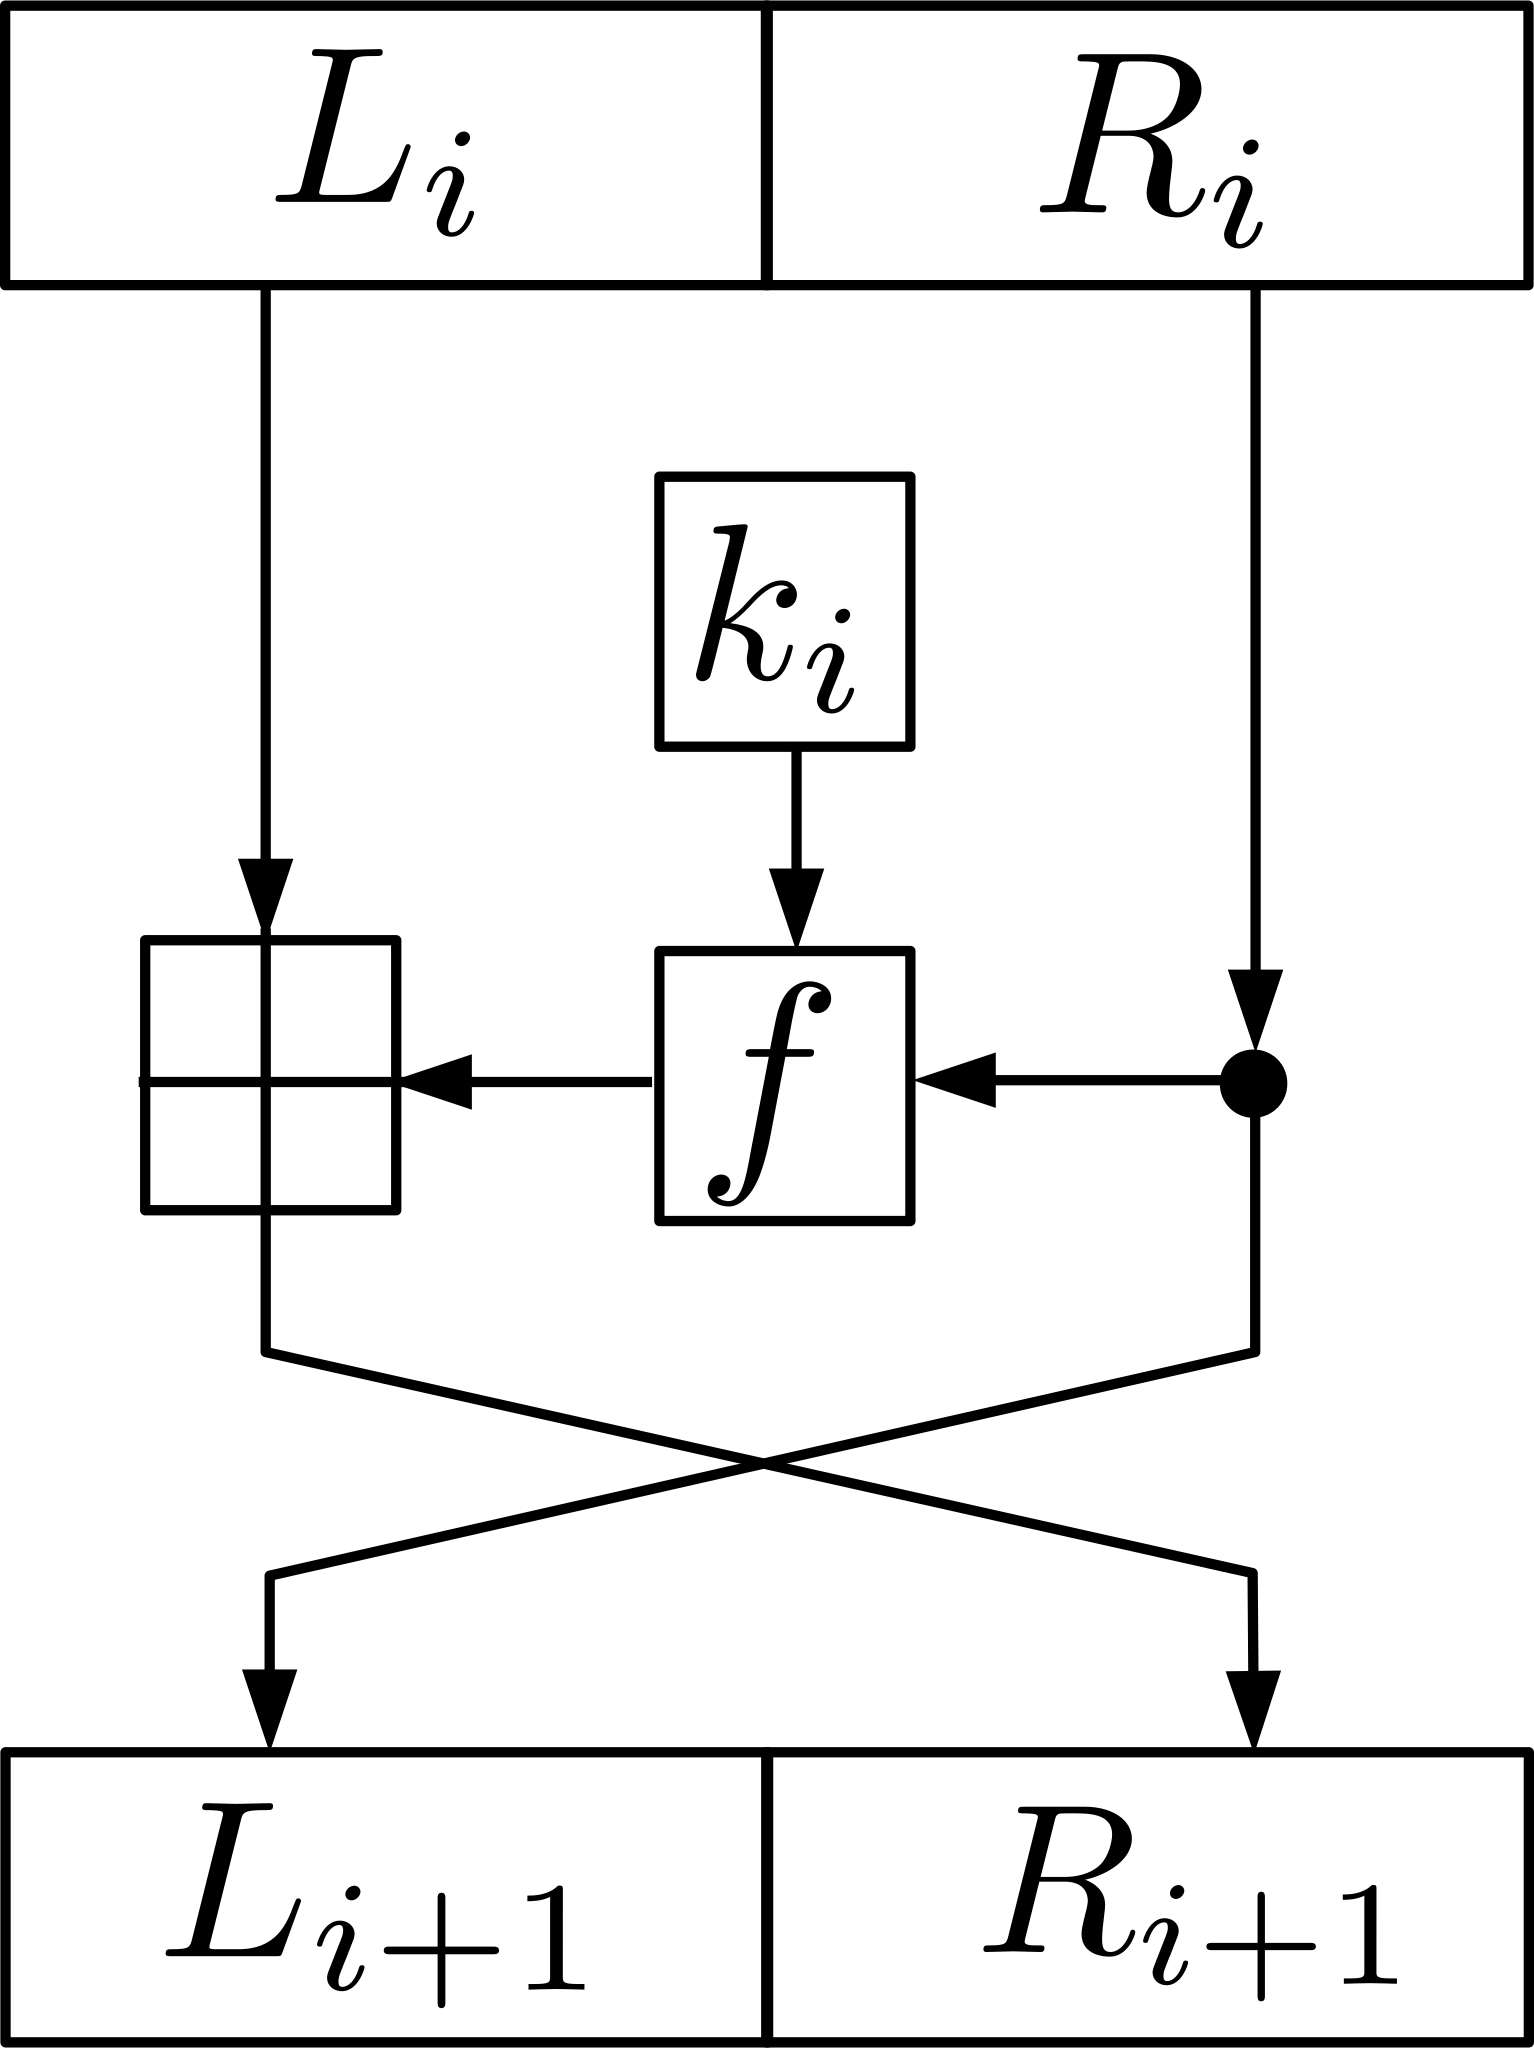
\includegraphics[width=.4\linewidth]{figures/feistel.pdf}
  \caption{Rodada de uma Rede de Feistel.}
  \label{fig:feistel}
\end{subfigure}%
\begin{subfigure}{.5\textwidth}
  \centering
  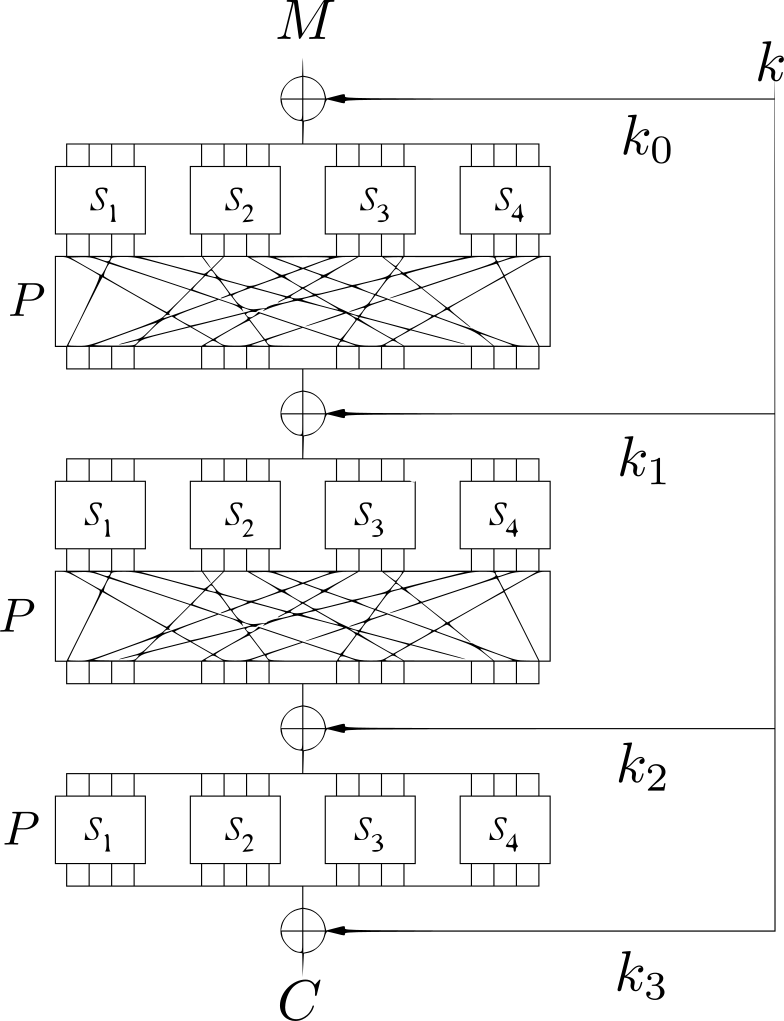
\includegraphics[width=.7\linewidth]{figures/spn.pdf}
  \caption{Rede de Permutação-Substituição.}
  \label{fig:spn}
\end{subfigure}
\caption{Construções para cifras de bloco.}
\label{fig:bloco}
\end{figure}

Cifras de fluxo, por sua vez, possuem construções derivadas de geradores pseudo-aleatórios, onde a chave criptográfica faz o papel da semente, a qual é expandida numa sequência pseudo-aleatória de bits, formando uma chave muito mais longa. Estas devem ser construídas de modo a maximizar o período do gerador, para evitar repetições na chave expandida. Pode-se dizer que cifras de fluxo são um relaxamento do \emph{one-time pad} (OTP), onde cada símbolo do texto claro é combinado com um símbolo aleatório da chave, que deve possuir o mesmo tamanho da mensagem a ser encriptada. A chave pseudo-aleatória de uma cifra de fluxo abre mão da \emph{segurança incondicional} do OTP~\cite{Shannon49}, em favor de uma premissa de segurança computacional com ganho de eficiência.

\subsubsection*{Modos de operação}

Modos de operação estendem o requisito de confidencialidade para mensagens de tamanho arbitrário, ou até mesmo requisitos de segurança adicionais, como \emph{encriptação autenticada}, em um único passo. Estes modos dividem a mensagem $M$ em $n$ blocos de mesmo tamanho $\{M_1, \ldots, M_n\}$ e utilizam uma regra para produzir os blocos de criptograma $C = \{C_1, \ldots, C_n\}$.
O último bloco precisa ser completado com \emph{preenchimento} (ou \emph{padding}) para poder ser processado corretamente.
Diversos modos de operação já foram padronizados por agências de padronização como o NIST para utilização governamental ou na indústria, dentre eles CBC, CTR e GCM.

No modo de operação CBC (\emph{Cipher Block Chaining}), o próximo bloco de criptograma é calculado a partir de um bloco de texto claro e o bloco de criptograma anterior, pela regra $C_i = E_k(M_i \oplus C_{i-1})$, para $2 \leq i \leq n$. O bloco $C_0$ é definido como um \emph{vetor de inicialização} $IV$ único e imprevisível, que não deve se repetir em encriptações distintas. Observe que o encadeamento da encriptação aleatoriza o bloco de texto claro antes da próxima encriptação, fazendo com que blocos idênticos produzam blocos distintos no criptograma. Como apenas a decriptação de blocos distintos pode ser feita de modo independente, paralelismo pode ser extraído apenas no processo de decriptação.

O modo de operação CTR (\emph{Counter} simula uma cifra de fluxo a partir de uma cifra de bloco. Os blocos do criptograma são calculados pela operação \texttt{XOR} entre blocos de texto claro e encriptação de valores consecutivos do vetor de inicialização $IV$. Portanto, a regra é dada por $C_i = M_i \oplus E_k(IV + i)$, para $1 \leq i \leq n$. Como o processamento de cada bloco é independente, este modo de operação oferece paralelismo tanto na encriptação quanto decriptação, sendo tipicamente mais eficiente que o modo CBC. A Figura~\ref{fig:modos} ilustra os dois modos de operação.

\begin{figure}[htbp]
\centering
\begin{subfigure}{\textwidth}
  \centering
  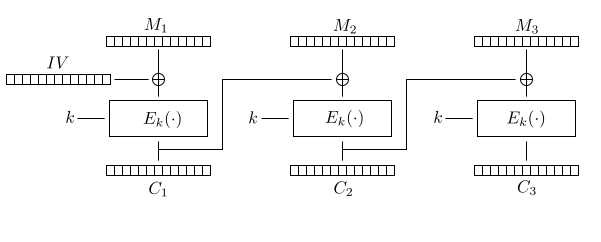
\includegraphics[width=.75\linewidth]{figures/cbc.pdf}
  \caption{Encriptação no modo CBC.}
  \label{fig:cbc}
\end{subfigure}
\begin{subfigure}{\textwidth}
  \centering
  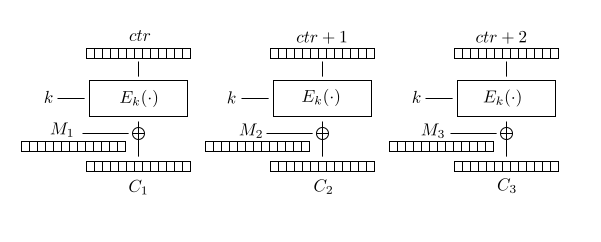
\includegraphics[width=.75\linewidth]{figures/ctr.pdf}
  \caption{Encriptação no modo CTR.}
  \label{fig:ctr}
\end{subfigure}
\caption{Modos de operação para cifras de bloco.}
\label{fig:modos}
\end{figure}

O modo de encriptação autenticada \emph{GCM} (\emph{Galois/Counter Mode})~\cite{McGrewV04} utiliza o modo CTR para encriptação e atualiza um autenticador calculado a partir dos blocos de criptograma $C_i$ que permite detetar posteriormente qualquer manipulação do criptograma em trânsito, com alta probabilidade. Opcionalmente, o modo também autentica dados associados transmitidos às claras, funcionalidade útil para autenticar cabeçalhos de pacotes de rede ou outra informação pública cuja integridade deva ser preservada e possa ser verificada pelo destinatário.

\subsection{Funções de \emph{hash} ou resumo criptográfico}

O objetivo de funções de \emph{hash} ou resumo criptográfico é mapear uma cadeia de \emph{bits} de tamanho arbitrário em um \emph{resumo} com tamanho fixo em \emph{bits}. Este resumo tem como papel identificar unicamente a mensagem de entrada, servindo como uma espécie de ``impressão digital'' da mesma. São muitas as aplicações em Criptografia e Segurança Computacional de funções criptográficas: armazenamento seguro de senhas, esquemas de assinatura digital, verificação de integridade, derivação de chaves criptográficas, geração de números pseudo-aleatórios, projeto de cifras de fluxo e autenticadores, provas de trabalho de moedas criptográficas, entre outras. A Figura~\ref{fig:hash} apresenta essa funcionalidade abstrata de funções de resumo criptográfico.

\begin{figure}[htbp]
\begin{center}
    \includegraphics[scale=0.25]{figures/hash.pdf}
    \caption{Função de resumo criptográfico mapeando $M$ para o valor de resumo $H(M)$.}
    \label{fig:hash}
\end{center}
\end{figure}

Em termos matemáticos, funções de resumo são da forma $H : \{0,1\}^* \rightarrow \{0,1\}^n$. Ou seja, mapeiam uma pré-imagem $x$ de tamanho finito e arbitrário em um \emph{valor de hash} $y = H(x)$ de tamanho fixo. A princípio, tratam-se de funções não-chaveadas, ou seja, não-parametrizadas por uma chave criptográfica, mas é claro que podem ser utilizadas também para calcular resumos de informação secreta. Para haver interesse criptográfico, funções de resumo precisam satisfazer as três propriedades abaixo:

\begin{itemize}
 \item {\bf Resistência à pré-imagem}: Dada uma função de resumo criptográfico $H$ e um resumo $y$, deve ser computacionalmente inviável encontrar $x$ tal que $y = H(x)$. Em outras palavras, deve ser difícil ``inverter'' a função para um certo valor de resumo.
 \item {\bf Resistência à segunda pré-imagem}: Dado um resumo $y$ e uma mensagem $x$ tais que $y = H(x)$, deve ser computacionalmente inviável encontrar uma mensagem $x' \neq x$ tal que $H(x') = H(x) = y$. Ou seja, deve ser difícil encontrar uma segunda mensagem mapeada para o mesmo valor de resumo.
 \item {\bf Resistência a colisões}: Deve ser computacionalmente inviável encontrar mensagens $x, x'$ tais que $H(x) = H(x')$; ou seja, deve ser difícil encontrar duas mensagens que colidem sob $H$ para um mesmo valor de resumo.
\end{itemize}

Há muitas formas diferentes de se construir essas funções.
Observe que, pelo tamanho e natureza dos conjuntos de domínio e imagem, \emph{colisões} entre diferentes entradas sob uma função $h$ necessariamente irão existir. O desafio é projetar uma função que torne computacionalmente inviável encontrar essas colisões, mesmo que seu número seja infinito.
Classicamente, o paradigma Merkle-Damg\aa rd constrói uma função de resumo criptográfico resistente a colisão a partir de uma função de compressão $h$ com entrada de tamanho fixo, também resistente a colisão~\cite{Merkle79,Damgard89a}. Na Figura~\ref{fig:merkle}, a entrada $X$ é dividida entre $B$ blocos, com aplicação de preenchimento para formar o último bloco, e a saída da última função de compressão define o valor de resumo. Funções de resumo podem também ser construídas a partir de cifras de bloco~\cite{PreneelGV93}, ou problemas difíceis de Teoria dos Números, como a fatoração de inteiros.

\begin{figure}[htbp]
\begin{center}
    \includegraphics[scale=0.2]{figures/merkle.pdf}
    \caption{Construção Merkle-Damg\aa rd para funções de resumo criptográfico.}
    \label{fig:merkle}
\end{center}
\end{figure}

Um paradigma de construção que se tornou imensamente popular é a classe de \emph{esponjas criptográficas}. Uma esponja é uma função com estado interno $s$ de tamanho finito $b$, dividido em duas seções: a taxa de \emph{bits} de tamanho $r$ e a capacidade de tamanho $c$, tais que $b = c + r$. Completam a especificação uma função de permutação $f$ de tamanho fixo, que transforma o estado interno, e uma regra de preenchimento. Durante a inicialização, uma função esponja atribui o valor 0 ao estado interno e completa a mensagem de entrada para que seu tamanho seja múltiplo de $r$, de forma que a entrada possa ser dividida em blocos de tamanho $r$. A cada iteração da função, um novo bloco da entrada é adicionado a parte do estado interno pela operação \texttt{XOR} e o estado interno $s$ é substituído por $f(s)$. Em outras palavras, os blocos da entrada são absorvidos sucessivamente no estado interno. Na etapa final, toma-se $r$ \emph{bits} do estado interno por iteração até que a saída atinja um tamanho pré-determinado, alternando com novas aplicações da função de permutação $f(s)$. A resistência a colisões ou ataques de pré-imagem depende do tamanho $c$, tipicamente escolhido como duas vezes o nível de segurança desejado. A Figura~\ref{fig:sponge} apresenta a construção~\cite{BertoniDPA08}.

\begin{figure}[htbp]
\begin{center}
    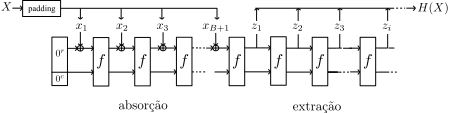
\includegraphics{figures/sponge.pdf}
    \caption{Esponja criptográfica, e suas fases de absorção e extração.}
    \label{fig:sponge}
\end{center}
\end{figure}

%%==============================================================
%%==============================================================

\section{Criptografia de curvas elípticas (ECC)}

%%==============================================================
%%==============================================================

%Criptografia de curvas elípticas é uma classe de algoritmos criptográficos que se baseia na aritmética de pontos de uma curva elíptica em um corpo finito $\mathbb{F}$ \cite{Hankerson:2003:GEC:940321}. Os algoritmos criptográficos que utilizam esse tipo de problema matemático podem se diferenciar de acordo com vários fatores, como por exemplo: o primo utilizado, a curva, corpo finito $\mathbb{F}_p$ ou $\mathbb{F}_{2^m}$, o mapeamento dos pontos na curva, entre outros. 

As operações mais simples executadas em uma curva é a adição de pontos e a duplicação de um ponto, sendo $R = P + Q$ e $R = P + P$ respectivamente. Dependendo da curva utilizada é possível executar essas operações de maneira mais eficiente podendo diferenciar o mapeamento desses pontos na curva.

Seguindo a notação descrita por \cite{Hankerson:2003:GEC:940321} podemos definir uma curva elíptica $E$ como: $E: y^2 + a_1xy + a_3y = x^3 + a_2x^2 + a_4x + a_6$ sobre um corpo K. Onde $\bigtriangleup \neq 0$, essa condição garante que não existirá ponto onde a curva possui duas ou mais linhas de tangente diferentes. A linha da tangente é utilizada na operação de duplicação de um ponto. Sendo que, $\bigtriangleup$ é definido como:

\begin{align*}
\bigtriangleup &= -d_2^2d_8 - 8d_4^3 - 27d_6^2 + 9d_2d_4d_6 \\
d_2 &= a_1^2 + 4a_2 \\
d_4 &= 2a_4 + a_1a_3 \\ 
d_6 &= a_3^2 + 4a_6 \\
d_8 &= a_1^2a_6 + 4a_2a_6 - a_1a_3a_4 + a_2a_3^2 - a_4^2
\end{align*}

A curva descrita anteriormente é chamada de equação de Weiertrass, onde a mesma possui uma forma simplificada: $y^2 = x^3 + ax + b$. Essa equação é utilizada como ponto inicial para descrição de várias curvas, sendo que pode-se variar os valores de $a$ e $b$ para obter diferentes curvas. Durante a escolha de qual utilizar é possível verificar a facilidade de implementação, possibilidade de paralelização, e também o desempenho da mesma. 

O desempenho está ligado as operações executadas, como por exemplo o método Montgomery-Ladder utilizado durante a multiplicação escalar, e pelas instruções do processador que facilitam a aritmética. Na seção a seguir iremos exibir as curvas com mais ocorrência na literatura, e algumas propriedades de cada uma.

\subsection{Curvas NIST e curvas modernas}
Primeiramente iremos apresentar as curvas NIST, essas curvas são recomendações de utilização feitas pelo NIST (National Institute of Standards and Technlogy), situado nos Estados Unidos da América. As mesmas foram geradas de forma pseudo-aleatória pela NSA, e possuem ao todo são 10 corpos finitos sendo 5 corpos primos ($\mathbb{F}_p$) e 5 corpos binários ($\mathbb{F}_{2^m}$) \cite{Brown2001}.

Os corpos foram recomendados com o foco no desempenho das curvas, facilitando a aritmética utilizada. Todavia existe uma resistência da comunidade em adotar o que foi proposto, pela incerteza na existência de vulnerabilidades, inseridas para obter informações secretas pelo governo norte americano. Os corpos finitos recomendados podem ser observados a seguir, sendo P os corpos primos e B as corpos binários:

\begin{multicols}{2}
\begin{itemize}
\item P-192 \\ $\mathbb{F}_{192}$ $p = 2^{192} - 2^{64} - 1$; 
\item P-224 \\ $\mathbb{F}_{224}$ $p = 2^{224} - 2^{96} + 1$;
\item P-256 \\ $\mathbb{F}_{256}$ $p = 2^{256} - 2^{224} + 2^{192} + 2^{96} - 1$;
\item P-384 \\ $\mathbb{F}_{384}$ $p = 2^{384} - 2^{128} - 2^{96} + 2^{32} - 1$;
\item P-521 \\ $\mathbb{F}_{521}$ $p = 2^{521} - 1$;
\item B-163 \\ $\mathbb{F}_{2^{163}}$ $f(x) = x^{163} + x^7 + x^6 + x^3 + 1$;
\item B-233 \\ $\mathbb{F}_{2^{233}}$ $f(x) = x^{233} + x^{74} + 1$;
\item B-283 \\ $\mathbb{F}_{2^{283}}$ $f(x) = x^{283} + x^{12} + x^7 + x^5 + 1$;
\item B-409 \\ $\mathbb{F}_{2^{409}}$ $f(x) = x^{409} + x ^{87} + 1$;
\item B-571 \\ $\mathbb{F}_{2^{571}}$ $f(x) = x^{571} + x^{10} + x^5 + x^2 + 1$.
\end{itemize}
\end{multicols}

Nesses corpos finitos primos é recomendado utilizar as curvas pseudo-aleatórias, já no caso dos corpos binários recomenda-se, além da utilização das curvas pseudo-aleatórias, o uso da curva de Koblitz. A geração de curvas pseudo-aleatórias segue três passos: primeiramente é gerada uma semente, após a partir da semente é gerada uma curva. Por fim, é verificado se a curva gerada é resistente aos ataques conhecidos, caso não seja o processo é repetido.

Existem duas curvas elípticas que estão se destacando considerando o desempenho obtido junto à técnicas de multiplicação escalar eficiente, redução modular, entre outras. Elas são a curva de Montgomery e a curva de Edwards, onde é possível encontrar implementações resistentes a ataques de canal lateral como ataque por tempo e ataque por cache.

A curva de Montgomery tem a seguinte equação: $E: y^2 = x^3 + Ax^2 + x$. O valor do parâmetro $A$ pode ser alterado para melhorar o desempenho das multiplicações escalares. Iremos tratar a utilização dessa curva com o primo $25519$ $(2^{255}-19)$ e o valor de $A = 486662$, dessa maneira a curva é definida sobre o corpo $\mathbb{F}_{2^{255}-19}$ \cite{Dull:2015:HCM:2834659.2834708}. Considerando o corpo finito utilizado essa curva é chamada de 25519, onde os pontos na curva são mapeados como $P = (X : Z)$. 

A curva de Edwards tem a fórmula: $E: -x^2 + y^2 = 1 + dx^2y^2$ \cite{Bernstein2012}. Nessa curva a soma de dois pontos segue a \textit{Edwards addition law}:
$$ (x_1,y_1) + (x_2,y_2) = (\frac{x_1y_2 + x_2y_1}{1 + xd_1x_2y_1y_2},\frac{y_1y_2 + x_1x_2}{1 - dx_1x_2y_1y_2}) $$%//TODO

Uma contramedida encontrada de fácil implementação para se tornar resistente a alguns ataques de canal lateral, como ataque de cache e hyperthreading, é possível apenas não escrever índices de dados secretos na memória RAM. Considerando que os ataques mencionados dependem das informações obtidas pela utilização dessas memórias eles não seriam efetivos. 

Um outro ataque conhecido é o ataque por tempo, o mesmo analisa o tempo de execução da primitiva criptográfico que utiliza a chave secreta, para tentar obter os bits da chave. A resistência do algoritmo está baseada na execução em tempo constante, o que pode ser obtido sem a utilização de branchs condicionais. Na seção 6 do minicurso iremos apresentar melhor essa contramedida e a eficácia da mesma.

\subsection{Algoritmos para multiplicação escalar (ECSM) básicos}

% Left-to-right binário (a.k.a. Point and Add Not-Always).
% Left-to-right binário com contramedida “Dummy Adds” de Coron  (a.k.a. Point and Add Always).
% Atomic Point and Add. Apresentar a idéia geral, e talvez um conjunto de fórmulas para uma dada curva como exemplo.
% Montgomery Ladder. Apenas a versão para curvas na forma de Montgomery.

Existem vários métodos para executar a multiplicação escalar, sendo que os mais simples de implementar serão apresentados nessa seção. O primeiro é o método \textit{Double-and-add}, o mesmo é utilizado para calcular $dP$. Ele possui quatro entradas, sendo $N$ uma variável para armazenar o resultado da operação de duplicação do ponto, Q armazena o resultado das operações, P é o ponto escolhido na curva para a multiplicação escalar, e por fim $d$ é a chave utilizada na multiplicação. É importante citar que $m$ é o tamanho da chave em bits, sendo que cada bit da chave será utilizado nesse método, totalizando 256 execuções para uma chave de 32 bytes.

\floatname{algorithm}{Algoritmo}
\begin{algorithm}[H]
\caption{Double-and-add}
\begin{algorithmic} 
    \REQUIRE $N, Q, P, d$
    \ENSURE $Q$
    \STATE $N \leftarrow P$
    \STATE $Q \leftarrow 0$
    \FOR{$i$ from $0$ \TO $m$} 
        \IF{$d_i = 1$}
            \STATE $Q \leftarrow addpoint(Q, N)$
        \ENDIF
        \STATE $N \leftarrow doublepoint(N)$
    \ENDFOR
    \RETURN Q
    \end{algorithmic}
\end{algorithm}


\subsection{Uso de tabelas precomputadas para melhorar desempenho; algoritmos de janela fixa}

\subsection{Algoritmos regulares; atomicidade; montgomery ladder}

Utilizando a curva de Montgomery é possível executar a multiplicação escalar pelo método chamado Montgomery Ladder. Esse método é dividido em degraus, sendo necessário executar 255 vezes para concluir a computação \cite{Dull:2015:HCM:2834659.2834708}.

\begin{algorithm}[H]
\caption{Montgomery ladder}
\begin{algorithmic} 
    \REQUIRE $s, x_p$
    \ENSURE $X_1, Z_1$
    \STATE $X_1 \leftarrow 1$
    \STATE $Z_1 \leftarrow 0$
    \STATE $X_2 \leftarrow x_p$
    \STATE $Z_2 \leftarrow 1$
    \STATE $p \leftarrow 0$
    \FOR{$i \leftarrow 254$ \TO $0$}
        \STATE $b \leftarrow s_i$
        \STATE $c \leftarrow b \oplus p$
        \STATE $p \leftarrow b$
        \STATE $(X_1, X_2) \leftarrow cswap(X_1,X_2,c)$
        \STATE $(Z_1,Z_2) \leftarrow cswap(Z_1,Z_2,c)$
        \STATE $(X_1, Z_1, X_2, Z_2) \leftarrow ladder(x_p, X_1, Z_1, X_2, Z_2)$
    \ENDFOR
    \RETURN $(X_1,Z_1)$
    \end{algorithmic}
\end{algorithm}

\begin{algorithm}[H]
\caption{Ladder}
\begin{multicols}{2}
\begin{algorithmic} 
    \REQUIRE $x_D, X_1, Z_1, X_2, Z_2$
    \ENSURE $X_1, Z_1, X_2, Z_2$
    \STATE $T_1 \leftarrow X_2 + Z_2$
    \STATE $X_2 \leftarrow X_2 - Z_2$
    \STATE $Z_2 \leftarrow X_1 + Z_1$
    \STATE $X_1 \leftarrow X_1 - Z_1$
    \STATE $T_1 \leftarrow T_1 \cdot X_1$
    \STATE $X_2 \leftarrow X_2 \cdot Z_2$
    \STATE $Z_2 \leftarrow Z_2 \cdot Z_2$
    \STATE $X_1 \leftarrow X_1 \cdot X_1$
    \STATE $T_2 \leftarrow Z_2 - X_1$
    \STATE $Z_1 \leftarrow T_2 \cdot a_24$
    
    
    \STATE $Z_1 \leftarrow Z_1 + X_1$
    \STATE $Z_1 \leftarrow T_2 \cdot Z_1$
    \STATE $X_1 \leftarrow Z_2 \cdot X_1$
    \STATE $Z_2 \leftarrow Z_2 - X_2$
    \STATE $Z_2 \leftarrow Z_2 \cdot Z_2$
    \STATE $Z_2 \leftarrow Z_2 \cdot x_D$
    \STATE $X_2 \leftarrow T_1 + X_2$
    \STATE $X_2 \leftarrow X_2 \cdot X_2$
    
    \RETURN $(X_1,Z_1)$
\end{algorithmic}
\end{multicols}
\end{algorithm}

\subsection{Protocolos de IoT que envolvem ECC}
Em  1985,   Neal  Koblitz~\cite{Koblitz:1987:ECC}   e  Victor  Miller
\cite{Miller:1986:ECC}, de forma independente, propuseram a utilização
de curvas elípticas para  projetar criptossistemas de chave-pública. 

Curvas elípticas são definidas por equações cúbicas, como por exemplo $y^2 = x^3 - x$, onde os valores $x,y$ pertencem a uma estrutura algébrica chamada corpo, dos quais os números racionais, reais e complexos são exemplos. A Figura \ref{fig:curvas} ilustra duas curvas elipticas sobre o conjunto $\mathbb{R}$ dos reais. Curvas elípticas não são  importantes apenas para a Criptografia, mas também em outros ramos da Matemática como, por exemplo, na  prova do Último Teorema de Fermat.~\cite{Hankerson:2003:GEC:940321}.
\begin{figure}[htpb]
\centering
\begin{subfigure}{.5\textwidth}
  \centering
  \includegraphics[width=.6\linewidth]{figures/curve1.png}
  \caption{$y^2 = x^3 -x + 1$}
  \label{fig:sub1}
\end{subfigure}%
\begin{subfigure}{.5\textwidth}
  \centering
  \includegraphics[width=.6\linewidth]{figures/curve2.png}
  \caption{$y^2 = x^3 - x$}
  \label{fig:sub2}
\end{subfigure}
\caption{Exemplo de duas curvas elípticas}
\label{fig:curvas}
\end{figure}
No caso da Criptografia de Curvas Elípticas (ECC), o corpo sobre o qual curvas são definidas são os chamados corpos finitos. Tais corpos são conjuntos finitos de tamanho $p^m$, denotados $\mathbb{F}_{p^m}$, onde $p$ um número primo e $m$ um inteiro maior ou igual a 1, e munidos de duas operações $+, \times$. Os elementos de $\mathbb{F}_{p^m}$ são os polinômios de grau máximo $m-1$ e coeficientes em $Z_p=\{0,1,2,\ldots,p-1\}$. 
As operações $+, \times$ são as operações usuais de adição e multiplicação de polinômios, com duas condições extras: (i) os coeficientes do polinômio $r(x)$ resultante de uma operação são reduzidos módulo $p$; e (ii) $r(x)$ é tomado módulo um polinômio irredutível $f(x)$ em $Z_p$.

Quando $m=1$, dizemos $\F_p$ é um corpo primo e seus elementos são simplesmente os inteiros em $\Z_p=\{0,1,2,\ldots,p-1\}$ com aritmética módulo $p$. A seguir  apresentaremos equações de curvas elípticas  para corpos primos $\Z_p$ e \emph{corpos binários} $\FF_{2^m}$.
%
\subsection*{Curvas sobre $\FF_p$ e $\F_{2^m}$}
Uma \emph{curva elíptica} $E$ sobre $\F_p$ é definida por uma equação da forma
\begin{equation}
\label{eq:cce}
y^2 = x^3 + ax + b,
\end{equation}
\noindent onde os coeficientes $a,b  \in \F_p$ satisfazem $4a^3 + 27b^2
\not\equiv 0 \pmod p$. Para corpos binários $\F_{2^m}$, uma
curva elíptica (não-supersingular) é definida por uma equação da forma
\begin{equation}
\label{eq:cce2}
y^2 + xy = x^3 + ax^2 + b,
\end{equation}
\noindent onde os  coeficientes $a,b \in \FF_{2^m}$ e  $b\neq 0$.  Dizemos
 que um  par $(x,y)$, onde $x,y \in \FF_q$ $(\F_p$ ou $\FF_{2^m})$,  é um \emph{
 ponto}  na  curva se  $(x,y)$  satisfaz  a  equação \ref{eq:cce}  (ou
 \ref{eq:cce2}).  O conjunto  de pontos  da curva  junto com  um ponto
 especial {$\infty$}, chamado \emph{ ponto no infinito}, é denotado por
 $E(\FF_q)$.   Por  exemplo,  se $E$  é  a  curva
 elíptica sobre $\Z_{29}$, definida pela equação
\begin{equation}
\label{eq:cce-exemplo-primo}
y^2 = x^3 + 4x + 20,
\end{equation}
\noindent então o conjunto de 37 pontos de $E(\FF_{29})$ é
\[
\begin{array}{lllllll}
\{{\infty}, & (2,6), & (4,19), & (8,10), & (13,23), & (16,2), & (19,16),  \\
(0,7), & (2,23), & (5,7), & (8,19), & (14,6), & (16,27), & (20,3),  \\
(0,22), & (3,1), & (5,22), & (10,4), & (14,23), & (17,10), & (20,26),  \\
(1,5), & (3,28), & (6,12), & (10,25), & (15,2), & (17,19), & (24,7), \\
(1,24), & (4,10), & (6,17), & (13,6), & (15,27), & (19,13), & (24,22),  \\
(27,2), & (27,27)\}. & & & & & 
\end{array}
\]
\noindent 

%%exemplo binário?
\noindent  Existe uma  operação, conhecida  como lei  de  ``secantes e
tangentes'', que  permite ``somar'' pontos elípticos em  $E$. Com essa
operação, o conjunto  de pontos de $E(\FF_q)$ forma  um grupo abeliano
cuja identidade é o ponto no infinito {$\infty$}.  A fórmula para somar
pontos  requer  umas  poucas  operações aritméticas  no  corpo  finito
subjacente.  Para  corpos primos  $\F_p$, as fórmulas  explícitas para
somar dois pontos são dadas a seguir:

\begin{enumerate}
\item {\it Identidade:} $P + {\infty} =  {\infty} + P = P$ para todo $P\in E(\F_p)$
\item \emph{Negativos:} Se $P = (x,y) \in E(\F_p)$ então $(x,y) + 
      (x,-y) = {\infty}$.\\
      O ponto $(x,-y)$ é denotado por $-P$ e chamado o {\it negativo} de $P$.
\item \emph{Soma de pontos:} Seja $P = (x_1,y_1)\in  E(\F_p)$ e 
$Q = (x_2,y_2)\in  E(\F_p)$, onde $P \neq \pm Q$. Então 
$P + Q = (x_3,y_3)$, onde 
\[ x_3 = (\frac{y_2-y_1}{x_2-x_1})^2 - x_1 - x_2\ \ {\rm{e}}\ \ 
   y_3 = (\frac{y_2-y_1}{x_2-x_1})(x_1-x_3)-y_1.\]
\item \emph{Duplicação de  ponto:} Seja $P = (x_1,y_1)\in  E(\F_p)$, onde 
$P \neq -P$. Então 
$2P = P + P = (x_3,y_3)$, onde 
\[ x_3 = (\frac{3x_1^2+a}{2y_1})^2 - 2x_1\ \ {\rm{e}}\ \ 
   y_3 = (\frac{3x_1^2 + a}{2y_1})(x_1-x_3)-y_1.\]
\end{enumerate}

A partir da operação de  soma no grupo $E(\FF_q)$, define-se o produto
de um escalar $k \in \Z$ por  um ponto $P \in E(\FF_q)$ como o ponto $
kP = P + P + \dots + P$  (com $k$ parcelas) se $k > 0$, e por extensão
$0P = {\infty}$  e $-kP = k(-P) = -(kP)$.  Esta  operação é chamada de
{\it multiplicação de um ponto por  um escalar} e é a operação central
dos esquemas criptográficos baseados em curvas elípticas. Quando estiver subentendido o corpo sobre o qual a curva $E(\F_{p^m})$ é  definida, escreveremos simplesmente $E$ para denotar a curva.

\ignore{
\begin{comment}
Curvas elípticas são definidas por equações cúbicas, como por exemplo $y^2 = x^3 - x$, onde os valores $x,y$ pertencem a uma estrutura algébrica chamada corpo, dos quais os números racionais, reais e complexos são exemplos. A Figura \ref{fig:curvas} ilustra duas curvas elipticas sobre o conjunto $\mathbb{R}$ dos reais. Curvas elípticas não são  importantes apenas para a Criptografia, mas também em outros ramos da Matemática como, por exemplo, na  prova do Último Teorema de Fermat.~\cite{Hankerson:2003:GEC:940321}.
\begin{figure}[htpb]
\centering
\begin{subfigure}{.5\textwidth}
  \centering
  \includegraphics[width=.6\linewidth]{figures/curve1.png}
  \caption{$y^2 = x^3 -x + 1$}
  \label{fig:sub1}
\end{subfigure}%
\begin{subfigure}{.5\textwidth}
  \centering
  \includegraphics[width=.6\linewidth]{figures/curve2.png}
  \caption{$y^2 = x^3 - x$}
  \label{fig:sub2}
\end{subfigure}
\caption{Exemplo de duas curvas elípticas}
\label{fig:curvas}
\end{figure}
No caso da Criptografia de Curvas Elípticas (ECC), o corpo sobre o qual curvas são definidas são os chamados corpos finitos. Tais corpos são conjuntos finitos de tamanho $p^m$, denotados $\mathbb{F}_{p^m}$, onde $p$ um número primo e $m$ um inteiro maior ou igual a 1, e munidos de duas operações $+, \times$. Os elementos de $\mathbb{F}_{p^m}$ são os polinômios de grau máximo $m-1$ e coeficientes em $Z_p=\{0,1,2,\ldots,p-1\}$. Isto é,
\[ \]
As operações $+, \times$ são as operações usuais de adição e multiplicação de polinômios, com duas condições extras: (i) os coeficientes do polinômio $r(x)$ resultante de uma operação são reduzidos módulo $p$; e (ii) $r(x)$ é tomado módulo um polinômio irredutível $f(x)$ em $Z_p$. Vejamos um exemplo em $\mathbb{F}_{2^3}$:

 existem são compostos por polinômios de grau finito  numa aritmética peculiar entre os pontos de uma curva elíptica em um corpo finito $\mathbb{F}_q$~\cite{Hankerson:2003:GEC:940321}, que definiremos a seguir. Os algoritmos criptográficos que utilizam esse tipo de problema matemático podem se diferenciar de acordo com vários fatores como, por exemplo, a curva e seu modelo, a escolha entre corpo finito primo $\mathbb{F}_p$ ou binário $\mathbb{F}_{2^m}$, o sistema de coordenadas, entre outros.

Seguindo a notação de~\cite{Hankerson:2003:GEC:940321},   definimos uma curva elíptica $E$ por $E: y^2 + a_1xy + a_3y = x^3 + a_2x^2 + a_4x + a_6$, onde os $a_i$ são elementos de um corpo finito K. Isto é são polinômios de grau e o discriminante $\bigtriangleup$, definido a seguir, deve ser não nulo. 


A operação central em ECC é a multiplicação por escalar (ECSM), descrita como $Q = kP$. As operações mais simples executadas em uma curva são a adição e a duplicação de pontos, isto é, $R = P + Q$ e $R = 2P$ respectivamente. Dependendo da curva utilizada, essas operações são computadas de formas diferentes, podendo fazer uso de propriedades específicas da curva para obter melhor desempenho.

Seguindo a notação de~\cite{Hankerson:2003:GEC:940321},   definimos uma curva elíptica $E$ por $E: y^2 + a_1xy + a_3y = x^3 + a_2x^2 + a_4x + a_6$, onde os $a_i$ são elementos de um corpo finito K e o discriminante $\bigtriangleup$, definido a seguir, deve ser não nulo. 
%\begin{comment}
Essa condição garante que não existirá ponto onde a curva possui duas ou mais linhas de tangente diferentes. A linha da tangente é utilizada na operação de duplicação de um ponto e o discriminante $\bigtriangleup$ é definido como:
%\end{comment}

\begin{align*}
\bigtriangleup &= -d_2^2d_8 - 8d_4^3 - 27d_6^2 + 9d_2d_4d_6, \mbox{ onde } \\
d_2 &= a_1^2 + 4a_2 \\
d_4 &= 2a_4 + a_1a_3 \\ 
d_6 &= a_3^2 + 4a_6 \\
d_8 &= a_1^2a_6 + 4a_2a_6 - a_1a_3a_4 + a_2a_3^2 - a_4^2
\end{align*}

A curva descrita anteriormente é chamada de equação de Weierstrass, e simplifica-se,  em muitos casos, para $y^2 = x^3 + ax + b$ e, portanto, $\bigtriangleup = -16(4a^3 +27b^2) \ne 0$. Diferentes escolhas para $a$ e $b$ produzem diferentes curvas. Tais escolhas podem afetar o desempenho e a segurança de implementações,  

%\begin{comment}
Essa equação é utilizada como ponto inicial para descrição de várias curvas, sendo que pode-se variar os valores de $a$ e $b$ para obter diferentes curvas. Durante a escolha de qual utilizar é possível verificar a facilidade de implementação, possibilidade de paralelização, e também o desempenho da mesma. 

O desempenho está ligado às operações executadas, como por exemplo o método \emph{Montgomery Ladder} utilizado durante a multiplicação por escalar, e pelas instruções do processador que facilitam a aritmética. 
%\end{comment}

Na seção a seguir exibiremos as curvas mais utilizadas, bem como algumas de suas propriedades.
\end{comment}
}

\subsection{Curvas NIST e curvas modernas}

As curvas NIST foram geradas pela NSA (National Security Agency) dos EUA e recomendadas para utilização pelo governo americano. São dez escolhas para corpos finitos, sendo cinco corpos primos ($\mathbb{F}_p$) e cinco corpos binários ($\mathbb{F}_{2^m}$)~\cite{Brown2001}. Os corpos finitos recomendados são relacionados a seguir, com os respectivos polinômios irredutíveis, onde o prefixo P denota corpos primos e o B denota corpos binários:

\begin{multicols}{2}
\begin{itemize}
\item P-192 \\ $\mathbb{F}_{192}$ $p = 2^{192} - 2^{64} - 1$; 
\item P-224 \\ $\mathbb{F}_{224}$ $p = 2^{224} - 2^{96} + 1$;
\item P-256 \\ $\mathbb{F}_{256}$ $p = 2^{256} - 2^{224} + 2^{192} + 2^{96} - 1$;
\item P-384 \\ $\mathbb{F}_{384}$ $p = 2^{384} - 2^{128} - 2^{96} + 2^{32} - 1$;
\item P-521 \\ $\mathbb{F}_{521}$ $p = 2^{521} - 1$;
\item B-163 \\ $\mathbb{F}_{2^{163}}$ $f(x) = x^{163} + x^7 + x^6 + x^3 + 1$;
\item B-233 \\ $\mathbb{F}_{2^{233}}$ $f(x) = x^{233} + x^{74} + 1$;
\item B-283 \\ $\mathbb{F}_{2^{283}}$ $f(x) = x^{283} + x^{12} + x^7 + x^5 + 1$;
\item B-409 \\ $\mathbb{F}_{2^{409}}$ $f(x) = x^{409} + x ^{87} + 1$;
\item B-571 \\ $\mathbb{F}_{2^{571}}$ $f(x) = x^{571} + x^{10} + x^5 + x^2 + 1$.
\end{itemize}
\end{multicols}

Os corpos foram determinados com base no desempenho, facilitando a aritmética utilizada. Há também opções de curvas binárias genéricas (ou de Koblitz) para as curvas binárias. As curvas acima foram geradas de forma pseudo-aleatória, descartando-se curvas que não fossem resistentes aos ataques conhecidos. Nem todas as etapas do processo de geração das curvas são completamente transparentes, especialmente na escolha de sementes do gerador de bits pseudo-aleatórios. Essa lacuna tem produzido resistência na comunidade técnica, por haver a possibilidade de que as sementes tenham sido escolhidas de forma a produzir curvas com vulnerabilidades conhecidas pela NSA mas desconhecidas do público em geral.

Por esse motivo, outros modelos de curvas elípticas têm recebido maior atenção na literatura científica e na adoção pela indústria, por terem métodos de geração mais transparentes e implementações de alto desempenho e protegidas contra ataques de canal lateral de tempo. Exemplos dessas são as curvas de Montgomery e Edward. Nessas curvas, o número de operações realizadas é \emph{regular} e baseiam-se apenas no comprimento das chaves e não no valor dos \emph{bits} da chave.

A curva de Montgomery é dada pela equação $E: y^2 = x^3 + Ax^2 + x$. O valor de $A$ pode ser alterado de forma a melhorar o desempenho das multiplicações escalares. O corpo primo mais utilizado com essa curva é $\mathbb{F}_{2^{255}-19}$ com o valor de $A = 486662$~\cite{Dull:2015:HCM:2834659.2834708}. Essa combinação possibilita a implementação eficiente da multiplicação por escalar usando o método de \emph{Montgomery Ladder}.

A curva de Edwards é encontrada na literatura na sua forma \emph{twisted}, em razão do desempenho exibido na combinação com os primos de Mersenne $p = 2^{127} - 1$ e $2^{255 - 10}$ em ~\cite{longa:2015} e~\cite{Bernstein2012}, respectivamente. A equação dessa curva é $-x^2 + y^2 = 1 + dx^2y^2$, onde $d$ é um não-quadrado em $\mathbb{F}_p^2$.

Nessa curva, a soma de dois pontos segue a fórmula de adição de ~\emph{Edwards}:
$$ (x_1,y_1) + (x_2,y_2) = (\frac{x_1y_2 + x_2y_1}{1 + xd_1x_2y_1y_2},\frac{y_1y_2 + x_1x_2}{1 - dx_1x_2y_1y_2}) $$
Um fato interessante é que a duplicação de um ponto tem a mesma fórmula da adição, o que não acontece em geral.

\subsection{Algoritmos básicos para multiplicação por escalar (ECSM)}

Como já dissemos, a principal operação em curvas elípticas é a multiplicação por escalar $kP$. O escalar $k$ é, de fato, a chave privada, ou parte dela, em vários esquemas criptográficos baseados em ECC. Dessa forma, é necessário explorar diferentes formas de implementar esse cálculo, não só do ponto de vista de desempenho como o de segurança, assunto central deste texto. Nesta seção serão apresentados os métodos mais simples para o cálculo de $kP$, resistentes ou não a ataques de canal lateral, e pequenas variações.

O primeiro é o método \textit{Double-and-add} (também conhecido como \textit{Double-and-add-not-always})~\cite{DBLP:journals/iacr/Rivain11}. 
\begin{comment}
Trabalha com quatro variáveis, onde $N$ armazena  o resultado da operação de duplicação do ponto durante a execução, $Q$ armazena o resultado final da operação, $P$ é o ponto escolhido na curva para a multiplicação por escalar, e por fim $k$ é a chave utilizada na multiplicação.

Para uma chave de 32 bytes o  importante citar que $m$ é o tamanho da chave em \emph{bits}, sendo que cada \textit{bit} da chave será utilizado nesse método, totalizando 256 execuções para uma chave de 32 {bytes}.
\end{comment}
O Algoritmo 1 é chamado de \textit{left-to-right, double-and-add} já que os bits de $k$ são processados da esquerda para a direita. Esse algoritmo não é resistente a ataques de canal lateral. Uma simples inspeção do código revela que o comando na linha 5 terá tempos de execução diferentes dependendo do valor do bit $k_i$. 

\floatname{algorithm}{Algoritmo}
\begin{algorithm}[H]
\caption{Left-to-right double-and-add}
\begin{algorithmic}[1] 
    \REQUIRE $P \in E(\mathbb{F}_p), k=(k_{t-1},\ldots,k_1,k_0)_2 \in \mathbb{N}$
    \ENSURE $kP \in E(\mathbb{F}_p)$
    \STATE $N \leftarrow P$
    \STATE $Q \leftarrow 0$
    \FOR{$i$ from $t-1$ \textbf{downto} $0$} 
        \STATE $N \leftarrow 2N$
        \IF{$k_i = 1$}
            \STATE $Q \leftarrow Q+N$
        \ENDIF
    \ENDFOR
    \RETURN Q
    \end{algorithmic}
\end{algorithm}

Uma outra maneira de percorrer os \textit{bits} de $k$ é da direita para a esquerda, conhecida como \textit{right-to-left}~\cite{DBLP:journals/iacr/Rivain11}, resultando num algoritmo ligeiramente diferente, o Algoritmo 2. Pelas mesmas razões acima, esse algoritmo não resiste a ataques de canal lateral de tempo. 

\floatname{algorithm}{Algoritmo}
\begin{algorithm}[H]
\caption{Right-to-left double-and-add}
\begin{algorithmic}[1]
    \REQUIRE $P \in E(\mathbb{F}_p), k=(k_{t-1},\ldots,k_1,k_0)_2 \in \mathbb{N}$
    \ENSURE $kP \in E(\mathbb{F}_p)$
    \STATE $N \leftarrow P$
    \STATE $Q \leftarrow 0$
    \FOR{$i$ from $0$ \TO $t-1$} 
        \IF{$k_i = 1$}
            \STATE $Q \leftarrow Q + N$
        \ENDIF
        \STATE $N \leftarrow 2N$
    \ENDFOR
    \RETURN Q
    \end{algorithmic}
\end{algorithm}

Mais adiante trataremos de outros métodos de multiplicação por escalar que são resistentes a ataques de canal lateral, tornando constante o número de operações executadas em cada iteração e o tempo de execução independente do valor do escalar $k$.

\subsection{Algoritmos para multiplicação de ponto fixo por escalar}

Nos casos em que $P$ é um ponto fixo, isto é, reutilizado para diferentes valores de $k$, é possível pré-processar parte da  multiplicação escalar $kP$, obtendo um ganho de desempenho~\cite{Hankerson:2003:GEC:940321}.

A ideia é pré-computar os valores $2^wP,\, 2^{2w}P,\, 2^{3w}P,\,\ldots,\, 2^{w(d-1)}P$, onde onde $w$ é o tamanho da palavra do processador-alvo da implementação, usualmente 32 ou 64 bits, também chamada de janela ou \emph{window} em inglês, e $d$ é o número de tais palavras ocupadas pelo escalar $k$~\cite{Hankerson:2003:GEC:940321}; isto é, se $k=(k_{t-1}, \ldots, k_1, k_0)_2$ tem $k$ bits, então $d=\lceil t/w \rceil$, e escrevemos $k=(K_{d-1}, \ldots, K_1, K_0)_{2^w}$ para denotar os blocos de $w$ bits da chave $k$. 

Utilizar janelas é uma prática comum para aumento da eficiência de implementações, já que operandos podem ser descritos e manipulados em blocos de bits do tamanho da janela, para o qual as instruções do processador já são especializadas. O Algoritmo~3, proposto por Brickell at al. utiliza essa técnica, conhecida por \textit{Fixed-base Windowing Method} .

\renewcommand{\algorithmicforall}{\textbf{for each}}
\floatname{algorithm}{Algoritmo}
%\label{alg:Brickell-etal}
\begin{algorithm}[H]
\caption{\emph{Fixed-base windowing method} para multiplicação escalar de um ponto}
\begin{algorithmic}[1]
    \REQUIRE Janela $w$, $P \in E(\mathbb{F}_p),\, d=\lceil t/w \rceil,\, k=(K_{d-1},\ldots,K_1,K_0)_{2^w} \in \N$
    \ENSURE $kP \in E(\mathbb{F}_p)$
    \STATE Compute $P_i = 2^{i}P, 0 \le i \le d-1$ (\emph{pré-computação})
    \STATE $A \leftarrow \infty$, \, $B \leftarrow \infty$
    \FOR{$j$ from $2^w-1$ \textbf{downto} $1$} 
        \FOR{\textbf{each} $i$ for which $K_i = j$}
            \STATE $B \leftarrow B + P_i$
            \STATE $A \leftarrow A + B$
        \ENDFOR
    \ENDFOR
    \RETURN A
    \end{algorithmic}
\end{algorithm}

\subsection{Algoritmos regulares para multiplicação por escalar}
Para que algoritmos de multiplicação por escalar sejam resistentes a ataques de canal lateral é necessário que o fluxo de execução seja regular, isto é, que não haja variações de tempo em função do valor do escalar $k$, a chave privada.

O primeiro exemplo dessa regularidade é ilustrada no Algoritmo 4, chamado \textit{Double-and-add-always} e proposto por Coron~\cite{Coron1999}, que executa uma adição e uma duplicação elípticas em todas a iterações. Uma implementação mais uniforme é a chamada \textit{Atomic Double-and-Add}~\cite{BatinaChmielewski2014}, que executa somente operações de soma de pontos elípticos.

\begin{algorithm}[H]
\caption{Double-and-add-always}
\begin{algorithmic}[1]
    \REQUIRE $P \in E(\mathbb{F}_p),\, k=(k_{t-1},\ldots,k_1,k_0)_{2} \in \N$
    \ENSURE $kP \in E(\mathbb{F}_p)$
    \STATE $R_0 \leftarrow P$
    \FOR{$i$ from $t-2$ \textbf{downto} $0$} 
        \STATE $R_0 \leftarrow 2R_0$
        \STATE $R_1 \leftarrow R_0 + P$
        \STATE $b \leftarrow k_{i}$
        \STATE $R_0 \leftarrow R_b$
    \ENDFOR
    \RETURN $R_0$
    \end{algorithmic}
\end{algorithm}

\begin{algorithm}[H]
\caption{Atomic double-and-add}
\begin{algorithmic}[1]
    \REQUIRE $P \in E(\mathbb{F}_p),\, k=(k_{t-1},\ldots,k_1,k_0)_{2} \in \N$
    \ENSURE $kP \in E(\mathbb{F}_p)$
    \STATE $R_0 \leftarrow P$
    \STATE $R_1 \leftarrow P$
    \STATE $j \leftarrow t - 2$
    \STATE $b \leftarrow 0$
    \WHILE{$j \ge 0$} 
        \STATE $R_0 \leftarrow R_0 + R_b$
        \STATE $b \leftarrow b \oplus k_j$
        \STATE $j \leftarrow j + k_j -1$
    \ENDWHILE
    \RETURN $R_0$
    \end{algorithmic}
\end{algorithm}

Um outro algoritmo importante é o chamado \textit{Montgomery Ladder}~\cite{Dull:2015:HCM:2834659.2834708}, que é mais eficiente que outros similares, e tem a vantagem adicional de poder ser otimizado para diferentes curvas. Primeiramente exibimos uma implementação genérica do método, no Algoritmo~6.

\begin{algorithm}[H]
\caption{\emph{Montgomery Ladder}}
\begin{algorithmic}[1]
    \REQUIRE $P \in E(\mathbb{F}_p), k=(k_{t-1},\ldots,k_1,k_0)_2 \in \mathbb{N}$
    \ENSURE $kP \in E(\mathbb{F}_p)$
    \STATE $R_0 \leftarrow P$
    \STATE $R_1 \leftarrow 2P$
    \FOR{$j \leftarrow t - 2$ \TO $0$} 
        \STATE $b \leftarrow k_j$
        \STATE $R_{1-b} \leftarrow R_0 + R_1$
        \STATE $R_b \leftarrow 2R_b$
    \ENDFOR
    \RETURN $R_0$
    \end{algorithmic}
\end{algorithm}

Quando se usa o \textit{Montgomery Ladder} com a curva de Montgomery com primo $p=2^{255}-19$, há um ganho de eficiência. Para o cálculo de $kP$, as entradas para o algoritmo são o escalar $k$ com 256 bits, e a coordenada $x_P$ do ponto $P$. A função \textit{cswap}, ou \textit{conditional swap}, faz a troca dos valores dos dois primeiros parâmetros caso o valor do terceiro parâmetro seja $1$.

\ignore{possui uma implementação mais eficiente para a curva  Na mesma, esse método é dividido em degraus, sendo necessário os executar 255 vezes para concluir a computação~\cite{Dull:2015:HCM:2834659.2834708}. São utilizadas duas entradas sendo $k$ o escalar com tamanho ($d$) igual a 256 \textit{bits}, e $x_p$ a coordenada $x$ do ponto a ser multiplicado. A função \textit{cswap}, conhecida como \textit{conditional swap}, faz a troca dos valores dos dois primeiros parâmetros caso o valor de $c$ seja $1$. Essa primeira parte do algoritmo pode ser observada no Algoritmo~7.
}

\begin{algorithm}[H]
\caption{\emph{Montgomery ladder} particularizado para a curva de Montgomery}
\begin{algorithmic}[1]
    \REQUIRE Coordenada $x_P$ de um ponto $P\in E(\mathbb{F}_p), k=(k_{255},\ldots,k_1,k_0)_2 \in \mathbb{N}$.
    \ENSURE $(X_1,Z_1)$ tais que a coordenada $x_{kP}$ de $kP$ é igual a $X_1/Z_1$. 
    \STATE $X_1 \leftarrow 1$
    \STATE $Z_1 \leftarrow 0$
    \STATE $X_2 \leftarrow x_P$
    \STATE $Z_2 \leftarrow 1$
    \STATE $r \leftarrow 0$
    \FOR{$i \leftarrow 254$ \TO $0$}
        \STATE $b \leftarrow k_i$
        \STATE $c \leftarrow b \oplus r$
        \STATE $r \leftarrow b$
        \STATE $(X_1, X_2) \leftarrow cswap(X_1,X_2,c)$
        \STATE $(Z_1,Z_2) \leftarrow cswap(Z_1,Z_2,c)$
        \STATE $(X_1, Z_1, X_2, Z_2) \leftarrow ladder(x_P, X_1, Z_1, X_2, Z_2)$
    \ENDFOR
    \RETURN $(X_1,Z_1)$
    \end{algorithmic}
\end{algorithm}

A função \emph{ladder}, detalhada no Algoritmo~8, calcula uma duplicação seguida por uma adição diferencial de pontos. Uma adição diferencial é uma adição de dois  pontos conhecendo-se sua diferença. Não justificaremos esse fato aqui, nos limitando à sua descrição. A operação não utiliza valores pré-calculados pré-armazenados, dificultando ataques de tempo na latência da hierarquia de memória (cache). A quantia~A na linha~10 é o coeficiente~$A$ da curva de Montgomery.

\begin{algorithm}[H]
\caption{Função \emph{ladder} - duplicação e adição diferencial de pontos}
\begin{multicols}{2}
\begin{algorithmic}[1]
    \REQUIRE $x, X_1, Z_1, X_2, Z_2$
    \ENSURE $X_1, Z_1, X_2, Z_2$
    \STATE $T_1 \leftarrow X_2 + Z_2$
    \STATE $X_2 \leftarrow X_2 - Z_2$
    \STATE $Z_2 \leftarrow X_1 + Z_1$
    \STATE $X_1 \leftarrow X_1 - Z_1$
    \STATE $T_1 \leftarrow T_1 \cdot X_1$
    \STATE $X_2 \leftarrow X_2 \cdot Z_2$
    \STATE $Z_2 \leftarrow Z_2 \cdot Z_2$
    \STATE $X_1 \leftarrow X_1 \cdot X_1$
    \STATE $T_2 \leftarrow Z_2 - X_1$
    \STATE $Z_1 \leftarrow T_2 \cdot (A+2)/4$
    
    
    \STATE $Z_1 \leftarrow Z_1 + X_1$
    \STATE $Z_1 \leftarrow T_2 \cdot Z_1$
    \STATE $X_1 \leftarrow Z_2 \cdot X_1$
    \STATE $Z_2 \leftarrow Z_2 - X_2$
    \STATE $Z_2 \leftarrow Z_2 \cdot Z_2$
    \STATE $Z_2 \leftarrow Z_2 \cdot x$
    \STATE $X_2 \leftarrow T_1 + X_2$
    \STATE $X_2 \leftarrow X_2 \cdot X_2$
    
    \RETURN $(X_1,Z_1,X_1,Z_2)$
\end{algorithmic}
\end{multicols}
\end{algorithm}

\subsection{Protocolos de IoT e ECC}

A necessidade por protocolos eficientes na Internet das Coisas é bem exemplificada no trabalho de Simplício et al.~\cite{SimplicioJr2016}, onde é descrita uma rede de sensores sem fio utilizando protocolos criptográficos baseados em ECC. Nós dessa rede têm baixa capacidade de recursos vitais como processamento, largura de banda, energia, memória, entre outros. Além do mais, sendo nós sensores autônomos, há boa chance de que sejam fisicamente monitorados ou manipulados por adversários.   Portanto, a comunicação entre os nós da rede requer não só implementações eficientes mas também robustas contra ataques por canais laterais, para que possam bem desempenhar suas funções em protocolos criptográficos  para acordo de chaves, encriptação e decriptação, entre outras funções de segurança. Descreveremos a seguir alguns ataques por canais laterais.

\ignore{
O protocolo de ECC descrito em~~\cite{SimplicioJr2016}  destina-se ao acordo de chaves autenticadas (iSMQV, do inglês \emph{Implicitly-Certified Authenticated Key Agreement}). Esse protocolo utiliza um centro gerador de chaves (KGC, do inglês \emph{Key Generation Center}) para gerar o par de chaves, pública e privada. Essas chaves possuem certificados que podem ser verificados com informações públicas. O objetivo desse protocolo é o estabelecimento de uma chave secreta entre dois nós da rede.
 
No protocolo iSMQV, para que o nó $A$ da rede obtenha o seu par de chaves, é necessário que se siga os seguintes passos:
\begin{enumerate}
    \item $A$ escolhe um número aleatório $\alpha$ e calcula $V = \alpha \cdot g$, onde $g$ é o gerador de um dado grupo $\mathbb{G}$, ambos públicos. $A$ envia $V$ e a sua identidade $ID_A$ para o KGC;
    \item O KGC executa as seguintes operações:
    \begin{enumerate}
     \item verifica a identidade de $A$ e calcula $V_A = V + \beta \cdot \mathbb{G}$, onde $\beta$ é um valor aleatório;
     \item calcula o hash $h = H(ID_A, V_A)$ e cria a assinatura $s = h \cdot \beta + r$;
     \item envia $s$ e $V_A$ para o nó $A$;
    \end{enumerate}      
    \item Por fim, $A$ calcula $h = H(ID_A, V_A)$, a chave privada $r_A = h \cdot \alpha + s$, e a chave pública $U_A = r_A \cdot G$.
\end{enumerate}

Após cada nó obter o seu par de chaves, estabelecem chaves simétricas com outros nós por meio do protocolo de Diffie-Hellman, usando na troca também suas identidades $ID_X$ e $Y$, para autenticarem-se mutuamente. 

Vamos apresentar o protocolo inteiro considerando dois nós que desejam se comunicar, $A$ e $B$. Cada nó escolhe um $x$ aleatório e computa $X = x \cdot G$. Esse resultado é trocado entre $A$ e $B$, e cada parte executa a multiplicação do seu $G$ pelo resultado do outro, sendo os resultados $s_A = X_B \cdot G$ e $s_B = X_A \cdot G$.

Após a troca da chave pública ela é validada e se for aprovada continuam o processo. Ambos $A$ e $B$ calculam os \textit{hashes} $d$ e $e$ da chave pública do outro e concatenam com a sua própria chave privada para computar $\sigma$. A chave secreta $K$ é computada criando um \textit{hash} de $\sigma$ e as informações públicas trocadas.

Esse é um exemplo de um protocolo com chave autenticada para acordo de chaves. É possível observar que com a utilização do protocolo Diffie-Hellman e a criptografia curvas elípticas é possível obter desempenho no acordo de chaves considerando o desempenho já apresentado nessa seção.
}

%%==============================================================
%%==============================================================

\section{Ataques de canal lateral}

%\subsection{Canal lateral (SCA) de tempo}

\subsubsection{O que é? Por que é importante?}
A premissa fundamental de ataques temporais \'{e} que o tempo gasto na execu\c{c}\~{a}o de uma instru\c{c}\~{a}o \'{e} influenciado por seus respectivos operandos \cite{ECCBook_HankersonVanstone2004}. Estudos mostraram \cite{1251354} a viabilidade desse ataque contra servidores executando protocolos como o SSL com RSA devido à lat\^{e}ncia da comunica\c{c}\~{a}o decorrente da rede local.

Como todos os ataques por canais laterais envolvem o monitoramento de uma grandeza f\'{i}sica, a limita\c{c}\~{a}o do \textit{time attack} \'{e} que as opera\c{c}\~{o}es com a chave criptogr\'{a}fica sejam \textit{lentas} o suficiente para serem medidas.

Acreditava-se que esse tipo de ataque seria poss\'{i}vel apenas em opera\c{c}\~{o}es de rede ou r\'{a}dio e jamais em processadores de disposit\'{i}vos m\'{o}veis ou se quer computadores justamente devido essa limita\c{c}\~{a}o.

Por\'{e}m uma forma derivada desse ataque denominada \textit{branch prediction analysis} (an\'{a}lise de preditor de salto) \cite{1266999} demonstrou ser poss\'{i}vel atacar uma implementa\c{c}\~{a}o do OpenSSL rodando em processadores convencionais (PowerPC, Intel, ARM, etc.).

Executando processos maliciosos em sistemas operacionais (Windows, Linux, Android, iOS, BlackBerry, etc.), foi demonstrado ser poss\'{i}vel afetar a execu\c{c}\~{a}o do OpenSSL. Tornando as itera\c{c}\~{o}es da exponencia\c{c}\~{a}o modular mais lentas, passando de nanosegundos para microsegundos, podem ser detecdadas e informações sobre a chave privada inferida.

\subsubsection*{Unidade de predi\c{c}\~{a}o de saltos}

As instru\c{c}\~{o}es que comp\~{o}em o c\'{o}digo bin\'{a}rio de um programa execut\'{a}vel podem consumir diferentes quantidades de ciclos de \textit{clock} de acordo com suas respectivas complexidades. Como no decorrer do fluxo de programas podem existir diversas depend\^{e}ncias entre as instru\c{c}\~{o}es executadas, existe a possibilidade de que valores necess\'{a}rios para a execu\c{c}\~{a}o de uma determinada instru\c{c}\~{a}o ainda n\~{a}o tenham sido calculados.

Quando a instru\c{c}\~{a}o depende um salto condicional, ent\~{a}o essa situa\c{c}\~{a}o \'{e} denominada \textit{control hazard}. Para que o processador n\~{a}o permane\c{c}a ocioso at\'{e} que o fluxo do programa seja definido, durante o per\'{i}odo de decis\~{a}o ele especula qual dever\'{a} ser a pr\'{o}xima instru\c{c}\~{a}o executada. Se a predi\c{c}\~{a}o se mostrar correta (\textit{hit}) o fluxo do programa prossegue sem degrada\c{c}\~{a}o de desempenho; caso a predi\c{c}\~{a}o se mostre incorreta (\textit{miss prediction}), o \textit{pipeline} deve ser esvaziado e a instru\c{c}\~{a}o correta tomada. Observe que uma \textit{miss prediction} acarreta em uma penalidade de ciclos de \textit{clock} que \'{e} proporcional \`{a} quantidade de est\'{a}gios do \textit{pipeline}.

Quando a CPU determina um salto como tomado, ela deve buscar a instru\c{c}\~{a}o do endere\c{c}o alvo do salto na mem\'{o}ria e entreg\'{a}-la a unidade de execu\c{c}\~{a}o. Para tornar o processo mais eficiente, a CPU mant\'{e}m um registro dos saltos executados anteriormente no BTB (\textit{Branch Target Buffer}). Observe que o tamanho do BTB \'{e} limitado; logo, alguns endere\c{c}os armazenados precisam ser expulsos para que novos endere\c{c}os sejam armazenados.
O preditor tamb\'{e}m possui uma parte denominada BHR (\textit{Branch History Registers}) respons\'{a}vel por gravar a hist\'{o}ria dos registradores usados globalmente e localmente pelo programa. \cite{Jean-Pierre06predictingsecret}.

\begin{figure}[ht]
	\centering
	\includegraphics[width=1\textwidth]{figures/automato.png}
	\caption{Aut\^{o}mato finito descreve o comportamento do preditor de saltos \cite{493986}.}
	\label{fig:Fig_automato}
\end{figure}

\begin{figure}[ht]
	\centering
	\includegraphics[width=.5\textwidth]{figures/btu.jpg}
	\caption{Unidade de predi\c{c}\~{a}o de saltos \cite{Jean-Pierre06predictingsecret}.}
	\label{fig:Fig_btu}
\end{figure}

\subsubsection*{Medi\c{c}\~{a}o direta de tempo}

A m\'{a}quina de estados que descreve as poss\'{i}veis decis\~{o}es da BTU possui um n\'{u}mero finito de estados; logo, o algoritmo que a descreve \'{e} determin\'{i}stico. O advers\'{a}rio pode assumir que a implementa\c{c}\~{a}o do RSA utilizou S\&M (\textit{Square-and-Multiply exponentiation algorithm}) e MM (\textit{Montgomery Multiplication algorithm} \cite{ECCBook_HankersonVanstone2004, 1197338}) e o BTU possui um aut\^{o}mato finito de apenas dois estados: salto tomado ou n\~{a}o tomado.

Seja $d$ a chave privada, vamos supor que o advers\'{a}rio conhece seus $i$ primeiros bits e est\'{a} tentando determinar $d_{i}$. Para qualquer mensagem $m$, o advers\'{a}rio pode simular as primeiras $i$ itera\c{c}\~{o}es e obter um resultado intermedi\'{a}rio que ser\'{a} a entrada da $(i+1)-$\textit{\'{e}sima} itera\c{c}\~{a}o. Ent\~{a}o ele gera quatro conjuntos distintos tais que:

\begin{align} \notag
	M_{1} = \left\lbrace m\ \vert\ d_{i} = 1 \rightarrow m\ causa\ missprediction\ durante\ MM\right\rbrace \\ \notag
	M_{2} = \left\lbrace m\ \vert\ d_{i} = 1 \rightarrow m\ causa\ hit\ durante\ MM\ \ \ \ \ \ \ \ \ \ \ \ \ \ \ \ \ \ \ \ \right\rbrace \\ \notag
	M_{3} = \left\lbrace m\ \vert\ d_{i} = 0 \rightarrow m\ causa\ missprediction\ durante\ MM\right\rbrace \\ \notag
	M_{4} = \left\lbrace m\ \vert\ d_{i} = 0 \rightarrow m\ causa\ hit\ durante\ MM\ \ \ \ \ \ \ \ \ \ \ \ \ \ \ \ \ \ \ \ \right\rbrace \\ \notag
\end{align}

O advers\'{a}rio calcula o tempo m\'{e}dio de execu\c{c}\~{a}o na multiplica\c{c}\~{a}o de Montgomery em cada conjunto $M_{i}$. Sendo $d_{i} = t, t \in \left\lbrace 0,1\right\rbrace $, a diferen\c{c}a dos tempos m\'{e}dios de execu\c{c}\~{a}o para o mesmo valor correto $t$ ser\~{a}o muito mais significativas do que a obtida dos outros dois conjuntos, pois, para o valor incorreto, os valores de tempo de cada multiplica\c{c}\~{a}o ter\~{a}o um caracter aleat\'{o}rio. Esse \'{e} o mesmo processo estat\'{i}stico da an\'{a}lise diferencial de pot\^{e}ncia. Portanto, se a diferen\c{c}a entre os tempos m\'{e}dios de $M_{1}$ e $M_{2}$ for muito mais significativa do que $M_{3}$ e $M_{4}$, ent\~{a}o o palpite correto \'{e} $d_{i} = 1$, e $d_{i} = 0$ caso contr\'{a}rio. 

Nesse ataque o advers\'{a}rio precisa saber de antem\~{a}o o estado do BPU antes do algoritmo de decripta\c{c}\~{a}o ser iniciado. Uma possibilidade de simples implementa\c{c}\~{a}o, por\'{e}m menos eficiente, seria realizar a an\'{a}lise supondo cada um dos quatro estados iniciais. A segunda abordagem consiste em for\c{c}ar o estado inicial do BPU de modo que nenhum endere\c{c}o de salto esteja no BTB. Essa abordagem ser\'{a} fundamentalmente a mesma utilizada em todos os ataques de predi\c{c}\~{a}o de salto listados a seguir.

\subsubsection*{For\c{c}ando BPU \`{a} mesma predi\c{c}\~{a}o assincronamente}

Unidades de processamento que permitem execu\c{c}\~{a}o concorrente de processos (SMT ou \textit{Simultaneous Multi-Threading} \cite{Silberschatz2004}) permitem que um advers\'{a}rio execute um processo espi\~{a}o simultaneamente ao programa de encripta\c{c}\~{a}o. Dessa forma, o advers\'{a}rio pode fazer com que o valor previsto dos saltos do encriptador nunca estejam no BTB; conseq\"{u}entemente, sempre ocorrer\'{a} um \textit{missprediction} quando o resultado correto, segundo a previs\~{a}o, seria que o salto fosse tomado. Comparado ao processo anterior, a an\'{a}lise diferencial seria similiar exceto pelo fato de que $d_{i} = 1$ em caso de \textit{hit} e $d_{i} = 0$ em caso de \textit{missprediction} durante o c\'{a}lculo de $m^{2} \bmod N$.

O processo espi\~{a}o remover do BTB o endere\c{c}o alvo de salto dos seguintes modos:
\begin{enumerate}
	\item (\textit{Total Eviction Method}: todas as entradas do BTB s\~{a}o expulsas.
	\item (\textit{Partial Eviction Method}): um conjunto de entradas do BTB \'{e} expulso.
	\item (\textit{Single Eviction Method}): apenas endere\c{c}o de interesse \'{e} expulso da tabela.
\end{enumerate}

Obviamente o primeiro m\'{e}todo \'{e} o de mais simples implementa\c{c}\~{a}o (assumindo que sejamos capazes de esvaziar todo o BTB entre duas itera\c{c}\~{o}es da exponencia\c{c}\~{a}o). O diferencial desse ataque \'{e} o advers\'{a}rio n\~{a}o ter que saber detalhes de implementa\c{c}\~{a}o da BPU para ser capaz de criar o processo espi\~{a}o e determinar quais s\~{a}o os bits da chave secreta.

\begin{figure}[ht]
	\centering
	\includegraphics[width=.7\textwidth]{figures/totaleviction.jpg}
	\caption{Resultados pr\'{a}ticos do \textit{Total Eviction Method} \cite{Jean-Pierre06predictingsecret}.}
	\label{fig:Fig_totaleviction}
\end{figure}

Esse ataque foi aplicado sobre uma implementa\c{c}\~{a}o do RSA em OpenSSL vers\~{a}o 0.9.7, rodando sob uma workstation RedHat 3. Foram gerados 10 milh\~{o}es de blocos de mensagens aleat\'{o}rias e chaves aleat\'{o}rias de $512$ bits. As mensagens foram encriptadas e separadas segundo os crit\'{e}rios acima, sendo assumido como tomado o salto do pr\'{o}ximo bit desconhecido.
       
Na Figura ~\ref{fig:Fig_totaleviction} (a), o eixo $x$ corresponde aos bits do expoente de 2 at\'{e} 511, sendo que cada coordenada $x_{i}$ apresenta os valores das m\'{e}dias das separa\c{c}\~{o}es correta e a m\'{e}dia das separa\c{c}\~{o}es aleat\'{o}rias, denotadas respectivamente por $\mu_{Y_{i}}$ e $\mu_{X_{i}}$. Analizando todos os pares $(\mu_{Y_{i}}, \mu_{X_{i}})$, o advers\'{a}rio verifica  qual deles teve a diferen\c{c}a mais significativa (Figura ~\ref{fig:Fig_totaleviction} (b)) e utiliza seus respectivos desvios padr\~{o}es para determinar o desvio da diferen\c{c}a das m\'{e}dias

\begin{align}\notag
    \mu_{Z} &= \mu_{Y} - \mu_{X} = 58.91 - 1.24 = 57.67\\\notag
    \sigma_{Z} &= \sqrt{ \sigma_{Y}^{2} + \sigma_{X}^{2}} = \sqrt{ 62.58^{2} - (34.78)^{2}} = 71.60\\ \notag
\end{align}

Sempre que o advers'{a}rio encontrar $Z > 0$, ele ir\'{a} supor que seu palpite do valor do \textit{bit} foi correta. O grau de certeza que o advers\'{a}rio pode ter nessas decis\~{o}es pode ser medido atrav\'{e}s da probabilidade:

\begin{align}
    Pr[Z > 0] = \phi(\dfrac{0 - \mu_{Z}}{\sigma_{Z}}) = \phi(-0.805) = 0.79\notag
\end{align}

Portanto, a probabilidade de suas decis\~{o}es estarem corretas para essas medidas \'{e} de quase 80\%, viabilizando o advser\'{a}rio obter o restante da chave por for\c{c}a bruta.

\subsubsection{Limitações}

\subsubsection{Impacto em IoT}

\subsection{Canal lateral de potência}

\subsubsection{Características gerais}
Em um ataque sobre o canal lateral de pot\^{e}ncia, o advers\'{a}rio analisa sutis varia\c{c}\~{o}es no consumo de energia el\'{e}trica de um dispositivo cujo \textit{hardware} implementa um algoritmo criptogr\'{a}fico (sensores RFID, \textit{smartcards}, \textit{SIM cards}, etc).

Opera\c{c}\~{o}es com dados sens\'{i}veis geram alter\c{c}\~{o}es na corrente ou tens\~{a}o da alimenta\c{c}\~{a}o do dispositivo, permitindo extrair parcialmente (ou mesmo integralmente) a chave criptogr\'{a}fica e outras informa\c{c}\~{o}es  sens\'{i}veis. O primeiro ataque dessa natureza foi apresentado por \cite{Kocher:1999:DPA:646764.703989}, tamb\'{e}m autor da c\'{e}lebre pesquisa precursora sobre \textit{time attacks} \cite{Kocher96}. 

\paragraph{Comparação entre canais laterais de potência e de tempo}

\subsubsection{Ataque de potência simples (SPA)}
A tecnologia de semicondutores dominante em microprocessadores, mem\'{o}rias e dispositivos embarcados \'{e} a CMOS   \cite{sedra:1997}, sendo inversores l\'{o}gicos sua unidade b\'{a}sica de constru\c{c}\~{a}o. Como dispositivos utilizam fontes constantes de tens\~{a}o, a pot\^{e}ncia consumida varia de acordo com o fluxo de sinais nos componentes, e esses de acordo com as opera\c{c}\~{o}es realizadas. Se esse consumo de pot\^{e}ncia for monitorado com aux\'{i}lio de um oscilosc\'{o}pio poderemos estabelecer um rastro de consumo de pot\^{e}ncia (\textit{power trace}) a cada ciclo do dispositivo.

\subsubsection{An\'{a}lise simples de pot\^{e}ncia sobre ECDSA}
Uma das rotinas mais executadas em dispositivos que utilizam ECC s\~{a}o os algoritmos de assinatura digital de curvas el\'{i}pticas (\textit{ECDSA} ou \textit{Elliptic Curve Digital Signature Algorithm}), tendo como opera\c{c}\~{a}o central a multiplica\c{c}\~{a}o de um ponto por um escalar (Algoritmo 8).

\floatname{algorithm}{Algoritmo}
\begin{algorithm}[H]
\caption{M\'{e}todo NAF bin\'{a}rio de multiplica\c{c}\~{a}o escalar de um ponto}
\begin{algorithmic}
    \REQUIRE $k \in \mathbb{N}$
    \REQUIRE $P \in E(\mathbb{F}_p)$
    \ENSURE $Q = kP \in E(\mathbb{F}_p)$
    \STATE $(k_{l-1}, k_{l-2}, ..., k_{1}, k_{0}) \leftarrow NAF(k)$
    \STATE $Q \leftarrow \infty$
    \FOR {$j \leftarrow l - 2$ \TO $0$}
        \STATE $Q \leftarrow 2Q$
        \IF {$k_{i} = 1$}
            \STATE $Q \leftarrow Q + P$
        \ENDIF
        \IF {$k_{i} = -1$}
            \STATE $Q \leftarrow Q - P$
        \ENDIF
    \ENDFOR
    \RETURN $Q$
    \end{algorithmic}
\end{algorithm}

\begin{figure}[ht]
	\centering
	\includegraphics[width=.8\textwidth]{figures/spa1.jpg}
	\caption{Consumo de pot\^{e}ncia durante c\'{a}lculo de $kP$ \cite{ECCBook_HankersonVanstone2004}.}
	\label{fig:Fig5}
\end{figure}

O que torna a forma n\~{a}o adjacente de $k$ mais interessante do que sua representa\c{c}\~{a}o bin\'{a}ria \'{e} o fato da $NAF(k)$ possuir apenas $1/3$ de d\'{i}gitos n\~{a}o nulos. Conseq\"{u}entemente uma quantidade muito menor de adi\c{c}\~{o}es (linhas $04$ e $05$ do Algoritmo 8) s\~{a}o efetuadas.

Entretanto um advers\'{a}rio que soubesse que o dispositivo implementa um algoritmo \textit{ECDSA} poderia monitorar o consumo de pot\^{e}ncia do dispositivo utilizando um oscilosc\'{o}pio, obtendo o gr\'{a}fico mostrado na Figura~\ref{fig:Fig5}. No Algoritmo 9, vemos que adi\c{c}\~{o}es s\~{a}o realizadas apenas quando $k_{i} \neq 0$; logo, uma maior quantidade de pot\^{e}ncia \'{e} despendida para d\'{i}gitos n\~{a}o nulos. Portanto os intervalos curtos denominados $D$ correspondem a itera\c{c}\~{o}es em que $k_{i} = 0$, enquanto intervalos longos denominados $S$ correspondem a itera\c{c}\~{o}es em que $k_{i} \neq 0$. Essa informa\c{c}\~{a}o torna vi\'{a}vel descobrir a chave atrav\'{e}s de ataques por for\c{c}a bruta, pois apenas $1/3$ dos d\'{i}gitos s\~{a}o n\~{a}o nulos.

A solu\c{c}\~{a}o mais simples contra SPA consiste em inserir opera\c{c}\~{o}es redundantes no algoritmo de multiplica\c{c}\~{a}o (Algoritmo 1.6), de modo que a seq\"{u}\^{e}ncia de opera\c{c}\~{o}es elementares envolvidas sejam realizadas em igual propor\c{c}\~{a}o. Comparando o novo \textit{power trace} obtido (Figura~\ref{fig:Fig7}) n\~{a}o \'{e} poss\'{i}vel diferenciar adi\c{c}\~{o}es de multiplica\c{c}\~{o}es.

\floatname{algorithm}{Algoritmo}
\begin{algorithm}[H]
\caption{M\'{e}todo NAF bin\'{a}rio de multiplica\c{c}\~{a}o escalar resistente \`{a} SPA}
\begin{algorithmic}
    \REQUIRE $k \in \mathbb{N}$
    \REQUIRE $P \in E(\mathbb{F}_p)$
    \ENSURE $Q = kP \in E(\mathbb{F}_p)$
    \STATE $(k_{l-1}, k_{l-2}, ..., k_{1}, k_{0}) \leftarrow NAF(k)$
    \STATE $Q \leftarrow \infty$\\
    \FOR {$i = l-1$ \TO $0$}
        \STATE $Q_{0} = 2Q_{0}$
        \STATE $Q_{1} = Q_{0} + P$
        \STATE $Q_{0} = Q_{k_{i}}$
    \ENDFOR
    \RETURN $Q$
    \end{algorithmic}
\end{algorithm}

\begin{figure}[ht]
	\centering
	\includegraphics[width=.8\textwidth]{figures/spa2.jpg}
	\caption{Consumo de pot\^{e}ncia durante c\'{a}lculo de $kP$ \cite{ECCBook_HankersonVanstone2004}.}
	\label{fig:Fig7}
\end{figure}

\subsubsection{Ataque de potência diferencial (DPA)}
Quando a varia\c{c}\~{a}o do consumo de pot\^{e}ncia n\~{a}o \'{e} sens\'{i}vel o suficiente em rela\c{c}\~{a}o as opera\c{c}\~{o}es executadas por um dispositivo, o advers\'{a}rio pode monitorar como o consumo varia em rela\c{c}\~{a}o ao valor de uma determinada vari\'{a}vel. Nesse ataque, primeiramente detectamos uma vari\'{a}vel $V$, influenciada, durante um processo de decripta\c{c}\~{a}o ou assinatura digital, por um texto $m$ e uma por\c{c}\~{a}o desconhecida  da chave privada. A partir disso, definimos a fun\c{c}\~{a}o de sele\c{c}\~{a}o $V = f(k',m)$.

O advers\'{a}rio ent\~{a}o coleta milhares de \textit{power traces}, determinando indutivamente todos os bits que comp\~{o}em a chave privada atrav\'{e}s do c\'{a}lculo da derivada dessa fun\c{c}\~{a}o. Para cada bit $k'_{i}$ corretamente previsto obtemos uma derivada n\~{a}o nula para os valores de $k'$ e $m$, caso contr\'{a}rio a derivada \'{e} nula. O processo \'{e} repetido at\'{e} que cada $k'_{i}$ seja determinando \cite{ECCBook_HankersonVanstone2004}. Esse modelo de ataque \'{e} conhecido como An\'{a}lise Diferencial de Pot\^{e}ncia (DPA ou \textit{Differential Power Analysis}).


\subsection{An\'{a}lise diferencial de pot\^{e}ncia sobre ECDSA}
Ainda que o Algoritmo 10 tenha sido adotado, podemos aplicar um DPA sobre o processo de ECDSA. 

Determinada uma vari\'{a}vel $V$ cujo valor influencie o consumo de pot\^{e}ncia e uma fun\c{c}\~{a}o de sele\c{c}\~{a}o $f$ tal que $V = f(k', m)$ o advers\'{a}rio coleta milhares de \textit{power traces}, estima o tamanho que a por\c{c}\~{a}o $k'$ ocupa na chave privada e separa os dados coletados em dois grupos de acordo com o valor previsto de $V$.

No algoritmo de multiplica\'{c}\~{a}o de pontos da curva el\'{i}ptica (Algoritmo 1.6), suponha que Eve colete \textit{power traces} durante os c\'{a}lculos $kP_{1} , kP_{2} , ..., kP_{r}$ . Como $P_{1} , P_{2} , ..., P_{r}$ s\~{a}o p\'{u}blicos, ele precisa determinar apenas $k$.

\begin{center}
    \begin{tabular}{|c|c|c|c|c|}
	    \hline
		    \   & $Q_{0}$  & $Q_{0}$ & $k_{t-1}$ & $Q_{0} \leftarrow Q_{k_{t-1}}$\\
	    \hline
	        $1$ & $\infty$ &     $P$ &       $1$ & $P$\\
	    \hline
		    $2$ & ... & ... & ... & ...\\
	    \hline
		    $3$ & ... & ... & ...& ... \\
	    \hline
		    ... & ... & ... & ...& ... \\
	    \hline
    \end{tabular}

    Tabela 1.2. $k = (1, k_{t-2}, k_{t-3}, ..., k_{1}, k_{0})$.
\end{center}

Dado $Q_{0} = \infty$, o passo 2.1 \'{e} trivial e pode ser disting\"{u}ir da de uma opera\c{c}\~{a}o n\~{a}o trivial
atrav\'{e}s do power trace, logo o advers\'{a}rio pode facilmente identificar o bit mais a esquerda cujo valor e 1. Tomando $k_{t-1}= 1$, na segunda itera\c{c}\~{a}o do algoritmo temos que $Q_{0} = 2P$ (se $k_{t-2} = 0$) ou $Q_{0} = 3P$ (se $k_{t-2} = 1$).

\begin{center}
    \begin{tabular}{|c|c|c|c|c|}
	    \hline
		    \   & $Q_{0}$  & $Q_{0}$ & $k_{t-1}$ & $Q_{0} \leftarrow Q_{k_{t-1}}$\\
	    \hline
	        $1$ & $\infty$ &     $P$ &       $1$ & $P$\\
	    \hline
		    $2$ & $2P$ & $4P$ & $\color{blue}{?}$ & $\color{blue}{?}$ \\
	    \hline
		    $3$ & ... & ... & ...& ... \\
	    \hline
		    ... & ... & ... & ...& ... \\
	    \hline
    \end{tabular}

    Tabela 1.3. $k = (1, k_{t-2}, k_{t-3}, ..., k_{1}, k_{0})$.
\end{center}

Conseq\"{u}entemente, na terceira itera\c{c}\~{a}o, o valor $4P$ ser computado apenas se $k_{t-2} = 0$. Definindo $k' = k_{t-2}$ e $m = P_{i}$ ($i$-\'{e}simo bit do ponto $4P = (4P_{1} , 4P_{2} , ..., 4P_{i} , ..., 4P_{r} , )$), a fun\c{c}\~{a}o seletora calcula o valor do bit $4P_{i}$.

\begin{center}
    \begin{tabular}{|c|c|c|c|c|}
	    \hline
		    \   & $Q_{0}$  & $Q_{0}$ & $k_{t-1}$ & $Q_{0} \leftarrow Q_{k_{t-1}}$\\
	    \hline
	        $1$ & $\infty$ &     $P$ &       $1$ & $P$\\
	    \hline
		    $2$ & $2P$ & $4P$ & $\color{red}{0}$ & $2P$ \\
	    \hline
		    $3$ & $\color{red}{4P}$ & $6P$ & ...& ... \\
	    \hline
		    ... & ... & ... & ...& ... \\
	    \hline
    \end{tabular}

    Tabela 1.4. $k = (1, \color{red}{0}$$,\ $$k_{t-3}, ..., k_{1}, k_{0})$.
\end{center}

Se o gr\'{a}fico do consumo de pot\^{e}ncia da fun\c{c}\~{a}o apresentar picos, ent\~{a}o $k_{t-2} = 0$, caso contr\'{a}rio $k_{t-2} = 1$.
Esse processo \'{e} repetido at\'{e} todos os bits de $k$ serem determinados \cite{ECCBook_HankersonVanstone2004}.

Se a curva el\'{i}ptica for gerada sobre um $\mathbb{F}_{p}$ de caracter\'{i}stica superior a 3, podemos usar um sistema misto de representa\c{c}\~{a}o de coordenadas no qual $P$ seja representado em um sistema de coordenadas afins, enquanto $Q_{0}$ e $Q_{1}$ s\~{a}o representados em coordenadas jacobianas \cite{ECCBook_HankersonVanstone2004}.

Se $P = (x,y)$ no sistema afim, ap\'{o}s a primeira atribui\c{c}\~{a}o $Q_{1} \leftarrow P$ ter\'{i}amos $ Q_{1} = (x : y : 1)$. Ent\~{a}o, $Q_{1}$ seria aleatorizado com $(\lambda^{2}x, \lambda^{3}y, \lambda)$ e o algoritmo procederia como o usual. Desse modo o advers\'{a}rio estaria impedido de realizar predi\c{c}\~{o}es baseadas no valor de um bit espec\'{i}fico $4P_{i}$ em sistemas de coordenadas jacobianas aleatorizadas.

\subsubsection{High-order DPA}

\subsubsection{Template attacks}
\subsection{Ataques temporais}

A premissa fundamental de ataques temporais \'{e} de que o tempo gasto na execu\c{c}\~{a}o de uma instru\c{c}\~{a}o \'{e} influenciado por seus respectivos operandos~\cite{ECCBook_HankersonVanstone2004}. Estudos mostraram~\cite{1251354} a viabilidade desse ataque contra servidores executando protocolos como o SSL com RSA devido à lat\^{e}ncia da comunica\c{c}\~{a}o decorrente da rede local.

Como todos os ataques por canais laterais envolvem o monitoramento de uma grandeza f\'{i}sica, um requisito para o sucesso de um ataque temporal \'{e} que as opera\c{c}\~{o}es com a chave criptogr\'{a}fica sejam \textit{lentas} o suficiente para serem medidas. Acreditava-se que esse tipo de ataque seria poss\'{i}vel apenas em opera\c{c}\~{o}es de rede ou r\'{a}dio e jamais em processadores de dispositivos m\'{o}veis ou  em computadores justamente devido a essa limita\c{c}\~{a}o.

Por\'{e}m, uma forma derivada desse ataque, denominada \textit{branch prediction analysis} (an\'{a}lise de preditor de salto)~\cite{1266999}, demonstrou ser poss\'{i}vel atacar uma implementa\c{c}\~{a}o do OpenSSL rodando em processadores convencionais (PowerPC, Intel, ARM, etc.). Executando processos maliciosos em sistemas operacionais (Windows, Linux, Android, iOS, BlackBerry, etc.), foi demonstrado ser poss\'{i}vel afetar a execu\c{c}\~{a}o do OpenSSL. Tornando as itera\c{c}\~{o}es da exponencia\c{c}\~{a}o modular mais lentas, passando de nanosegundos para microsegundos, foi possível detetar e inferir informações sobre a chave privada.

\subsubsection{Unidade de predi\c{c}\~{a}o de saltos}

As instru\c{c}\~{o}es que comp\~{o}em o c\'{o}digo bin\'{a}rio de um programa execut\'{a}vel podem consumir diferentes quantidades de ciclos de \textit{clock} de acordo com suas respectivas complexidades. Como no decorrer do fluxo de programas podem existir diversas depend\^{e}ncias entre as instru\c{c}\~{o}es executadas, existe a possibilidade de que valores necess\'{a}rios para a execu\c{c}\~{a}o de uma determinada instru\c{c}\~{a}o ainda n\~{a}o tenham sido calculados.

Quando a instru\c{c}\~{a}o depende de um salto condicional, essa situa\c{c}\~{a}o \'{e} denominada \textit{control hazard}. Para que o processador n\~{a}o permane\c{c}a ocioso at\'{e} que o fluxo do programa seja definido, durante o per\'{i}odo de decis\~{a}o especula-se qual dever\'{a} ser a pr\'{o}xima instru\c{c}\~{a}o executada. Se a predi\c{c}\~{a}o se mostrar correta (\textit{hit}), o fluxo do programa prossegue sem degrada\c{c}\~{a}o de desempenho; caso a predi\c{c}\~{a}o se mostre incorreta (\textit{miss prediction}), o \textit{pipeline} deve ser esvaziado e a instru\c{c}\~{a}o correta executada. Observe que uma \textit{miss prediction} acarreta em uma penalidade de ciclos de \textit{clock} que \'{e} proporcional \`{a} quantidade de est\'{a}gios do \textit{pipeline}.

Quando a CPU determina um salto como tomado (feito), ela deve buscar a instru\c{c}\~{a}o do endere\c{c}o-alvo do salto na mem\'{o}ria e entreg\'{a}-la à unidade de execu\c{c}\~{a}o. Para tornar o processo mais eficiente, a CPU mant\'{e}m um registro dos saltos executados anteriormente no BTB (\textit{Branch Target Buffer}). Observe que o tamanho do BTB \'{e} limitado; logo, alguns endere\c{c}os armazenados precisam ser removidos para que novos endere\c{c}os sejam armazenados.
O preditor tamb\'{e}m possui uma parte denominada BHR (\textit{Branch History Registers}) respons\'{a}vel por gravar a hist\'{o}ria dos registradores usados globalmente e localmente pelo programa~\cite{Jean-Pierre06predictingsecret}.

\begin{figure}[ht]
	\centering
	\includegraphics[width=0.7\textwidth]{figures/automato.png}
	\caption{Aut\^{o}mato finito descreve o comportamento do preditor de saltos~\cite{493986}.}
	\label{fig:Fig_automato}
\end{figure}

\begin{figure}[ht]
	\centering
	\includegraphics[width=.5\textwidth]{figures/btu.jpg}
	\caption{Unidade de predi\c{c}\~{a}o de saltos~\cite{Jean-Pierre06predictingsecret}.}
	\label{fig:Fig_btu}
\end{figure}

\subsubsection{Medi\c{c}\~{a}o direta de tempo}

A m\'{a}quina de estados que descreve as poss\'{i}veis decis\~{o}es da BTU possui um n\'{u}mero finito de estados; logo, o algoritmo que a descreve \'{e} determin\'{i}stico. O advers\'{a}rio pode supor que a implementa\c{c}\~{a}o do RSA utilizou S\&M (\textit{Square-and-Multiply exponentiation algorithm}) e MM (\textit{Montgomery Multiplication algorithm}~\cite{ECCBook_HankersonVanstone2004, 1197338}) e o BTU possui um aut\^{o}mato finito de apenas dois estados: salto tomado ou n\~{a}o tomado.

Seja $d$ a chave privada, e vamos supor que o advers\'{a}rio conheça seus $i$ primeiros bits e est\'{a} tentando determinar $d_{i}$. Para qualquer mensagem $m$, o advers\'{a}rio pode simular as primeiras $i$ itera\c{c}\~{o}es e obter um resultado intermedi\'{a}rio que ser\'{a} a entrada da $(i+1)-$\textit{\'{e}sima} itera\c{c}\~{a}o. Ent\~{a}o, ele gera quatro conjuntos distintos tais que:

\begin{align} \notag
	M_{1} = \left\lbrace m\ \vert\ d_{i} = 1 \rightarrow m\ \mbox{causa}\ missprediction\ \mbox{durante}\ MM\right\rbrace \\ \notag
	M_{2} = \left\lbrace m\ \vert\ d_{i} = 1 \rightarrow m\ \mbox{causa}\ hit\ \mbox{durante}\ MM\ \ \ \ \ \ \ \ \ \ \ \ \ \ \ \ \ \ \ \ \right\rbrace \\ \notag
	M_{3} = \left\lbrace m\ \vert\ d_{i} = 0 \rightarrow m\ \mbox{causa}\ missprediction\ \mbox{durante}\ MM\right\rbrace \\ \notag
	M_{4} = \left\lbrace m\ \vert\ d_{i} = 0 \rightarrow m\ \mbox{causa}\ hit\ \mbox{durante}\ MM\ \ \ \ \ \ \ \ \ \ \ \ \ \ \ \ \ \ \ \ \right\rbrace \\ \notag
\end{align}

O advers\'{a}rio calcula o tempo m\'{e}dio de execu\c{c}\~{a}o na multiplica\c{c}\~{a}o de Montgomery em cada conjunto $M_{i}$. Sendo $d_{i} = t, t \in \left\lbrace 0,1\right\rbrace $, então a diferen\c{c}a dos tempos m\'{e}dios de execu\c{c}\~{a}o para o mesmo valor correto $t$ ser\~{a}o muito mais significativas do que a obtida dos outros dois conjuntos, pois, para o valor incorreto, os valores de tempo de cada multiplica\c{c}\~{a}o ter\~{a}o um caráter aleat\'{o}rio. Portanto, se a diferen\c{c}a entre os tempos m\'{e}dios de $M_{1}$ e $M_{2}$ for muito mais significativa do que $M_{3}$ e $M_{4}$, ent\~{a}o o palpite correto \'{e} $d_{i} = 1$, e $d_{i} = 0$ caso contr\'{a}rio. 

Nesse ataque o advers\'{a}rio precisa saber de antem\~{a}o o estado do BPU antes do algoritmo de decripta\c{c}\~{a}o ser iniciado. Uma possibilidade simples de  implementa\c{c}\~{a}o, por\'{e}m menos eficiente, seria realizar a an\'{a}lise supondo cada um dos quatro estados iniciais. A segunda abordagem consiste em for\c{c}ar o estado inicial do BPU de modo que nenhum endere\c{c}o de salto esteja no BTB. Essa abordagem ser\'{a} fundamentalmente a mesma utilizada em todos os ataques de predi\c{c}\~{a}o de salto listados a seguir.

\subsubsection{For\c{c}ando BPU \`{a} mesma predi\c{c}\~{a}o assincronamente}

Unidades de processamento que permitem execu\c{c}\~{a}o concorrente de processos (SMT ou \textit{Simultaneous Multi-Threading}~\cite{Silberschatz2004}) permitem que um advers\'{a}rio execute um processo espi\~{a}o simultaneamente ao programa de encripta\c{c}\~{a}o. Dessa forma, o advers\'{a}rio pode fazer com que o valor previsto dos saltos do encriptador nunca estejam no BTB; conseq{u}entemente, sempre ocorrer\'{a} uma \textit{misprediction} quando o resultado correto, segundo a previs\~{a}o, seria que o salto fosse tomado. Comparado ao processo anterior, a an\'{a}lise diferencial seria similiar exceto pelo fato de que $d_{i} = 1$ em caso de \textit{hit} e $d_{i} = 0$ em caso de \textit{misprediction} durante o c\'{a}lculo de $m^{2} \bmod N$.

O processo espi\~{a}o remove do BTB o endere\c{c}o-alvo de salto das seguintes maneiras:
\begin{enumerate}
	\item (\textit{Total Eviction Method}: todas as entradas do BTB s\~{a}o removidas.
	\item (\textit{Partial Eviction Method}): um conjunto de entradas do BTB \'{e} removido.
	\item (\textit{Single Eviction Method}): apenas o endere\c{c}o de interesse \'{e} removido da tabela.
\end{enumerate}

Obviamente o primeiro m\'{e}todo \'{e} o de implementa\c{c}\~{a}o mais simples (assumindo que sejamos capazes de esvaziar todo o BTB entre duas itera\c{c}\~{o}es da exponencia\c{c}\~{a}o). O diferencial desse ataque \'{e} o advers\'{a}rio n\~{a}o ter que saber detalhes de implementa\c{c}\~{a}o da BPU para ser capaz de criar o processo espi\~{a}o e determinar quais s\~{a}o os bits da chave secreta.

\begin{figure}[ht]
	\centering
	\includegraphics[width=.7\textwidth]{figures/totaleviction.jpg}
	\caption{Resultados pr\'{a}ticos do \textit{Total Eviction Method}~\cite{Jean-Pierre06predictingsecret}.}
	\label{fig:Fig_totaleviction}
\end{figure}

Esse ataque foi aplicado sobre uma implementa\c{c}\~{a}o do RSA em OpenSSL vers\~{a}o 0.9.7, rodando sob uma workstation RedHat 3. Foram gerados 10 milh\~{o}es de blocos de mensagens aleat\'{o}rias e chaves aleat\'{o}rias de $512$ bits. As mensagens foram encriptadas e separadas segundo os crit\'{e}rios acima, sendo assumido como tomado o salto do pr\'{o}ximo bit desconhecido.
       
Na Figura ~\ref{fig:Fig_totaleviction} (a), o eixo $x$ corresponde aos bits do expoente de 2 at\'{e} 511, sendo que cada coordenada $x_{i}$ apresenta os valores das m\'{e}dias das separa\c{c}\~{o}es corretas e a m\'{e}dia das separa\c{c}\~{o}es aleat\'{o}rias, denotadas respectivamente por $\mu_{Y_{i}}$ e $\mu_{X_{i}}$. Analisando todos os pares $(\mu_{Y_{i}}, \mu_{X_{i}})$, o advers\'{a}rio verifica  qual deles teve a diferen\c{c}a mais significativa (Figura ~\ref{fig:Fig_totaleviction} (b)) e utiliza seus respectivos desvios padr\~{o}es para determinar o desvio da diferen\c{c}a das m\'{e}dias

\begin{align}\notag
    \mu_{Z} &= \mu_{Y} - \mu_{X} = 58.91 - 1.24 = 57.67\\\notag
    \sigma_{Z} &= \sqrt{ \sigma_{Y}^{2} + \sigma_{X}^{2}} = \sqrt{ 62.58^{2} - (34.78)^{2}} = 71.60\\ \notag
\end{align}

Sempre que o advers\'{a}rio encontrar $Z > 0$, ele ir\'{a} supor que seu palpite do valor do \textit{bit} foi correta. O grau de certeza que o advers\'{a}rio pode ter nessas decis\~{o}es pode ser medido pela probabilidade

\begin{align}
    Pr[Z > 0] = \phi(\dfrac{0 - \mu_{Z}}{\sigma_{Z}}) = \phi(-0.805) = 0.79.\notag
\end{align}
Portanto, a probabilidade de suas decis\~{o}es estarem corretas para essas medidas \'{e} de quase 80\%, possibilitando ao advers\'{a}rio obter o restante da chave por for\c{c}a bruta.

\subsection{Ataques de potência}

Em um ataque no canal lateral de pot\^{e}ncia, o advers\'{a}rio analisa sutis varia\c{c}\~{o}es no consumo de energia el\'{e}trica de um dispositivo cujo \textit{hardware} implementa um algoritmo criptogr\'{a}fico (sensores RFID, \textit{smartcards}, \textit{SIM cards}, etc).

Opera\c{c}\~{o}es com dados sens\'{i}veis geram altera\c{c}\~{o}es na corrente ou tens\~{a}o da alimenta\c{c}\~{a}o do dispositivo, permitindo extrair parcialmente (ou mesmo integralmente) a chave criptogr\'{a}fica e outras informa\c{c}\~{o}es  sens\'{i}veis. O primeiro ataque dessa natureza foi apresentado por~\cite{Kocher:1999:DPA:646764.703989}, tamb\'{e}m autor da c\'{e}lebre pesquisa precursora sobre \textit{time attacks}~\cite{Kocher96}. 

\subsubsection{Ataque de potência simples (SPA)}
A tecnologia de semicondutores dominante em microprocessadores, mem\'{o}rias e dispositivos embarcados \'{e} a CMOS~\cite{sedra:1997}, sendo inversores l\'{o}gicos sua unidade b\'{a}sica de constru\c{c}\~{a}o. Como dispositivos utilizam fontes constantes de tens\~{a}o, a pot\^{e}ncia consumida varia de acordo com o fluxo de sinais nos componentes, e esses de acordo com as opera\c{c}\~{o}es realizadas. Se esse consumo de pot\^{e}ncia for monitorado com aux\'{i}lio de um oscilosc\'{o}pio, poderemos estabelecer um rastro de consumo de pot\^{e}ncia (\textit{power trace}) a cada ciclo do dispositivo.

\subsubsection{An\'{a}lise simples de pot\^{e}ncia sobre ECDSA}
Uma das rotinas mais executadas em dispositivos que utilizam ECC s\~{a}o os algoritmos de assinatura digital de curvas el\'{i}pticas (\textit{ECDSA} ou \textit{Elliptic Curve Digital Signature Algorithm}), tendo como opera\c{c}\~{a}o central a multiplica\c{c}\~{a}o de um ponto por um escalar (Algoritmo~\ref{alg:NAFmult}).

\floatname{algorithm}{Algoritmo}
\begin{algorithm}[H]
\caption{Binary NAF method for scalar multiplication}
\begin{algorithmic}[1]
    \REQUIRE $P \in E(\mathbb{F}_p), k \in \mathbb{N}$
    \ENSURE $Q = kP \in E(\mathbb{F}_p)$
    \STATE $(k_{t-1}, k_{t-2}, ..., k_{1}, k_{0}) \leftarrow NAF(k)$
    \STATE $Q \leftarrow \infty$
    \FOR {$j \leftarrow t - 2$ \TO $0$}
        \STATE $Q \leftarrow 2Q$
        \IF {$k_{i} = 1$}
            \STATE $Q \leftarrow Q + P$
        \ENDIF
        \IF {$k_{i} = -1$}
            \STATE $Q \leftarrow Q - P$
        \ENDIF
    \ENDFOR
    \RETURN $Q$
    \end{algorithmic}
\label{alg:NAFmult}
\end{algorithm}

\begin{figure}[ht]
	\centering
	\includegraphics[width=.8\textwidth]{figures/spa1.jpg}
	\caption{Consumo de pot\^{e}ncia durante c\'{a}lculo de $kP$~ \cite{ECCBook_HankersonVanstone2004}.}
	\label{fig:Fig5}
\end{figure}

O que torna a forma n\~{a}o adjacente de $k$ mais interessante do que sua representa\c{c}\~{a}o bin\'{a}ria \'{e} o fato da $NAF(k)$ possuir apenas $1/3$ de d\'{i}gitos n\~{a}o nulos. Conseq{u}entemente uma quantidade muito menor de adi\c{c}\~{o}es (linhas $6$ e $9$ do Algoritmo 9) s\~{a}o efetuadas.

Entretanto um advers\'{a}rio que soubesse que o dispositivo implementa um algoritmo \textit{ECDSA} poderia monitorar o consumo de pot\^{e}ncia utilizando um oscilosc\'{o}pio, obtendo o gr\'{a}fico mostrado na Figura~\ref{fig:Fig5}. No Algoritmo 9, vemos que adi\c{c}\~{o}es s\~{a}o realizadas apenas quando $k_{i} \neq 0$; logo, uma maior quantidade de pot\^{e}ncia \'{e} despendida para d\'{i}gitos n\~{a}o nulos. Portanto os intervalos curtos denominados $D$ correspondem a itera\c{c}\~{o}es em que $k_{i} = 0$, enquanto intervalos longos denominados $S$ correspondem a itera\c{c}\~{o}es em que $k_{i} \neq 0$. Essa informa\c{c}\~{a}o torna vi\'{a}vel descobrir a chave por meio de ataques de for\c{c}a bruta, pois apenas $1/3$ dos d\'{i}gitos s\~{a}o n\~{a}o nulos.

A solu\c{c}\~{a}o mais simples contra SPA consiste em inserir opera\c{c}\~{o}es redundantes no algoritmo de multiplica\c{c}\~{a}o (Algoritmo~\ref{alg:NAFRegular}), de modo que a seq{u}\^{e}ncia de opera\c{c}\~{o}es elementares envolvidas sejam realizadas em igual propor\c{c}\~{a}o. Comparando o novo \textit{power trace} obtido (Figura~\ref{fig:Fig7}) n\~{a}o \'{e} poss\'{i}vel diferenciar adi\c{c}\~{o}es de multiplica\c{c}\~{o}es.

\floatname{algorithm}{Algoritmo}
\begin{algorithm}[H]
\caption{Binary NAF method for scalar multiplication resistant to SPA}
\begin{algorithmic}[1]
    \REQUIRE $P \in E(\mathbb{F}_p), k \in \mathbb{N}$
    \ENSURE $Q = kP \in E(\mathbb{F}_p)$
    \STATE $(k_{t-1}, k_{t-2}, ..., k_{1}, k_{0}) \leftarrow NAF(k)$
    \STATE $Q \leftarrow \infty$\\
    \FOR {$i = t-1$ \TO $0$}
        \STATE $Q_{0} = 2Q_{0}$
        \STATE $Q_{1} = Q_{0} + P$
        \STATE $Q_{0} = Q_{k_{i}}$
    \ENDFOR
    \RETURN $Q$
    \end{algorithmic}
\label{alg:NAFRegular}
\end{algorithm}

\begin{figure}[ht]
	\centering
	\includegraphics[width=.8\textwidth]{figures/spa2.jpg}
	\caption{Consumo de pot\^{e}ncia durante c\'{a}lculo de $kP$~\cite{ECCBook_HankersonVanstone2004}.}
	\label{fig:Fig7}
\end{figure}

\subsubsection{Ataque de potência diferencial (DPA)}
Quando a varia\c{c}\~{a}o do consumo de pot\^{e}ncia n\~{a}o \'{e} sens\'{i}vel o suficiente em rela\c{c}\~{a}o às opera\c{c}\~{o}es executadas por um dispositivo, o advers\'{a}rio pode monitorar como o consumo se comporta em rela\c{c}\~{a}o ao valor de uma determinada vari\'{a}vel. Nesse ataque, primeiramente detetamos uma vari\'{a}vel $V$, influenciada durante um processo de decripta\c{c}\~{a}o ou assinatura digital por um texto $m$ e uma por\c{c}\~{a}o desconhecida  da chave privada. A partir disso, definimos a fun\c{c}\~{a}o de sele\c{c}\~{a}o $V = f(k',m)$.

O advers\'{a}rio ent\~{a}o coleta milhares de \textit{power traces}, determinando indutivamente todos os bits que comp\~{o}em a chave privada atrav\'{e}s do c\'{a}lculo da derivada dessa fun\c{c}\~{a}o. Para cada bit $k'_{i}$ corretamente previsto obtemos uma derivada n\~{a}o nula para os valores de $k'$ e $m$, caso contr\'{a}rio a derivada \'{e} nula. O processo \'{e} repetido at\'{e} que cada $k'_{i}$ seja determinando~\cite{ECCBook_HankersonVanstone2004}. Esse modelo de ataque \'{e} conhecido como An\'{a}lise Diferencial de Pot\^{e}ncia (DPA ou \textit{Differential Power Analysis}).


\subsubsection{An\'{a}lise diferencial de pot\^{e}ncia sobre ECDSA}
Ainda que o Algoritmo~\ref{alg:NAFRegular} tenha sido adotado, podemos aplicar um DPA sobre o processo de ECDSA. 

Determinada uma vari\'{a}vel $V$ cujo valor influencie o consumo de pot\^{e}ncia, e uma fun\c{c}\~{a}o de sele\c{c}\~{a}o $f$ tal que $V = f(k', m)$, o advers\'{a}rio coleta milhares de \textit{power traces}, estima o tamanho que a por\c{c}\~{a}o $k'$ ocupa na chave privada e separa os dados coletados em dois grupos de acordo com o valor previsto de $V$.

Suponha que o adversário colete os \textit{power traces} durante os c\'{a}lculos de $kP_{1} , kP_{2} , ..., kP_{r}$, para os quais foi usado o Algoritmo~4  (\emph{Double-and-add always}), que repetimos aqui para facilitar a leitura.
\newcounter{foo}
\setcounter{foo}{\value{algorithm}}
\setcounter{algorithm}{3}
\begin{algorithm}[htb]
\caption{Double-and-add-always}
\begin{algorithmic}[1]
    \REQUIRE $P \in E(\mathbb{F}_p),\, k=(k_{t-1},\ldots,k_1,k_0)_{2} \in \N$
    \ENSURE $kP \in E(\mathbb{F}_p)$
    \STATE $R_0 \leftarrow P$
    \FOR{$i$ from $t-2$ \textbf{downto} $0$} 
        \STATE $R_0 \leftarrow 2R_0$
        \STATE $R_1 \leftarrow R_0 + P$
        \STATE $b \leftarrow k_{i}$
        \STATE $R_0 \leftarrow R_b$
    \ENDFOR
    \RETURN $R_0$
    \end{algorithmic}
\end{algorithm}
\setcounter{algorithm}{\value{foo}}

Como $P_{1} , P_{2} , ..., P_{r}$ s\~{a}o p\'{u}blicos, ele precisa determinar apenas $k$.
\begin{table}[htb]
\begin{center}
    \begin{tabular}{|c|c|c|c|c|}
	    \hline
		    \   & $R_{0}$  & $R_{0}$ & $k_{t-1}$ & $R_{0} \leftarrow R_{k_{t-1}}$\\
	    \hline
	        $1$ & $\infty$ &     $P$ &       $1$ & $P$\\
	    \hline
		    $2$ & ... & ... & ... & ...\\
	    \hline
		    $3$ & ... & ... & ...& ... \\
	    \hline
		    ... & ... & ... & ...& ... \\
	    \hline
    \end{tabular}
\caption{ $k = (1, k_{t-2}, k_{t-3}, ..., k_{1}, k_{0})$}
\end{center}
\end{table}
Dado $R_{0} = \infty$, o passo 3 do Algoritmo~4 \'{e} trivial e pode ser disting{u}ido de uma opera\c{c}\~{a}o n\~{a}o trivial pelo \emph{power trace}; logo, o advers\'{a}rio pode facilmente identificar o bit mais a esquerda cujo valor é 1. Tomando $k_{t-1}= 1$, na segunda itera\c{c}\~{a}o do algoritmo temos que $R_{0} = 2P$ (se $k_{t-2} = 0$) ou $R_{0} = 3P$ (se $k_{t-2} = 1$).
\begin{table}[htb]
\begin{center}
    \begin{tabular}{|c|c|c|c|c|}
	    \hline
		    \   & $R_{0}$  & $R_{0}$ & $k_{t-1}$ & $R_{0} \leftarrow R_{k_{t-1}}$\\
	    \hline
	        $1$ & $\infty$ &     $P$ &       $1$ & $P$\\
	    \hline
		    $2$ & $2P$ & $4P$ & $\color{blue}{?}$ & $\color{blue}{?}$ \\
	    \hline
		    $3$ & ... & ... & ...& ... \\
	    \hline
		    ... & ... & ... & ...& ... \\
	    \hline
    \end{tabular}
\caption{$k = (1, k_{t-2}, k_{t-3}, ..., k_{1}, k_{0})$}
\end{center}
\end{table}
Conseq{u}entemente, na terceira itera\c{c}\~{a}o, o valor $4P$ ser computado apenas se $k_{t-2} = 0$. Definindo $k' = k_{t-2}$ e $m = P_{i}$ ($i$-\'{e}simo bit do ponto $4P = (4P_{1} , 4P_{2} , ..., 4P_{i} , ..., 4P_{r} , )$), a fun\c{c}\~{a}o seletora calcula o valor do bit $4P_{i}$.
\begin{table}[htb]
\begin{center}
    \begin{tabular}{|c|c|c|c|c|}
	    \hline
		    \   & $R_{0}$  & $R_{0}$ & $k_{t-1}$ & $R_{0} \leftarrow R_{k_{t-1}}$\\
	    \hline
	        $1$ & $\infty$ &     $P$ &       $1$ & $P$\\
	    \hline
		    $2$ & $2P$ & $4P$ & $\color{red}{0}$ & $2P$ \\
	    \hline
		    $3$ & $\color{red}{4P}$ & $6P$ & ...& ... \\
	    \hline
		    ... & ... & ... & ...& ... \\
	    \hline
    \end{tabular}
\caption{$k = (1, \color{red}{0}$$,\ $$k_{t-3}, ..., k_{1}, k_{0})$}
\end{center}
\end{table}
Se o gr\'{a}fico do consumo de pot\^{e}ncia da fun\c{c}\~{a}o apresentar picos, ent\~{a}o $k_{t-2} = 0$, caso contr\'{a}rio $k_{t-2} = 1$.
Esse processo \'{e} repetido at\'{e} todos os bits de $k$ serem determinados~\cite{ECCBook_HankersonVanstone2004}.

Se a curva el\'{i}ptica for gerada sobre um $\mathbb{F}_{p}$ de caracter\'{i}stica superior a 3, podemos usar um sistema misto de representa\c{c}\~{a}o de coordenadas no qual $P$ seja representado em um sistema de coordenadas afins, enquanto $R_{0}$ e $R_{1}$ s\~{a}o~ representados em coordenadas jacobianas \cite{ECCBook_HankersonVanstone2004}.

Se $P = (x,y)$ no sistema afim, ap\'{o}s a primeira atribui\c{c}\~{a}o $R_{1} \leftarrow P$ ter\'{i}amos $ R_{1} = (x : y : 1)$. Ent\~{a}o, $R_{1}$ seria aleatorizado com $(\lambda^{2}x, \lambda^{3}y, \lambda)$ e o algoritmo procederia como o usual. Desse modo o advers\'{a}rio estaria impedido de realizar predi\c{c}\~{o}es baseadas no valor de um bit espec\'{i}fico $4P_{i}$ em sistemas de coordenadas jacobianas aleatorizadas.

\subsubsection{\emph{High-order DPA}}
Uma variação do ataque de potência diferencial é o \textit{high-order} DPA (HODPA), que é baseado em um conjunto de propriedades estatísticas do sinal de potência. Para obter uma melhor taxa de acerto dos \textit{bits} da chave, é necessária uma quantidade maior de amostras. Além disso, existe uma complexidade maior durante a implementação desse ataque~\cite{benedikt:2009:228}.

Um ponto importante a ser observado é que esse ataque possui a capacidade de se  sobrepor à resistência de uma contramedida de \textit{masking} e obter os \textit{bits} da chave. Isso é possível pela análise tanto do valor mascarado como da própria máscara criando uma relação entre ambos. Um problema encontrado na utilização desse ataque é a identificação do momento em que é necessário obter o sinal referente ao valor mascarado ou a máscara.

\subsubsection{\emph{Template attacks}}
O \textit{Template Attack} (TA) utiliza amostras de potência elétrica para executar uma análise, na tentativa de obter os \textit{bits} da chave privada. É  considerado o mais poderoso dentre os ataques de potência diferencial. Existe uma divisão em duas fases do ataque, a saber, a fase de construção e a fase de correlação. A primeira gera um \textit{template} de um padrão obtido no dispositivo alvo. Na segunda é analisada a correlação entre o \textit{template} gerado e as amostras obtidas durante a execução do dispositivo~\cite{ozgen:2016}. Esse ataque pode ser combinado com algoritmos de classificação para diferenciar valores da chave daqueles do restante, como é proposto no trabalho de~\cite{ozgen:2016}. Uma outra opção é a utilização de algoritmos de reconhecimento de padrão com aprendizado de máquina.

%%==============================================================
%%==============================================================

\section{Ataques e contramedidas para criptografia simétrica}

%\subsection{Utilização de CPA em implementação do AES}

\subsection{Contramedida de mascaramento}

\subsection{Ataques e contramedidas para MACs baseados em funções de
hash}
Implementações inseguras de criptografia simétrica podem ser suscetíveis a diversos tipos de ataques
de canal lateral. Mesmo implementações de algoritmos de alto desempenho podem ser vulneráveis a canais
laterais de tempo executados localmente (via latência da memória \emph{cache}) ou remotamente
(tempo de resposta na comunicação em rede). Contramedidas comuns para criptografia simétrica contra ataques de canal lateral
envolvem execução em tempo constante e mascaramento.

\subsection{Ataques por canal lateral de tempo e contramedidas}

Um ataque simples contra a utilização de criptografia simétrica envolve a aplicação de funções de resumo criptográfico
para autenticação. Nessas aplicações, é comum que o algoritmo simétrico produza um autenticador ou \emph{hash} das credenciais
que precisa ser comparado com o resultado correto. Durante a comparação de cadeias de caracteres,
pequenas variações no tempo de execução podem fornecer informação útil para o adversário reduzir enormemente a complexidade de um
ataque de busca exaustiva. Ao comparar cadeias, se a interrupção do laço acontecer exatamente na primeira posição diferente,
o adversário é capaz de realizar um ataque de busca exaustiva em cada \emph{byte} individualmente,
baseado no tempo de resposta. Desta forma, é possível determinar o autenticador de uma mensagem ou \emph{hash} de uma senha, por exemplo,
sem conhecimento de segredos. O trecho de código abaixo ilustra uma forma segura de comparação, cujo tempo de execução é invariante e saturado para o pior caso:

\begin{center}
\begin{verbatim}
int cmp_const(const void * a, const void * b,
              const size_t size) {
    const unsigned char *_a = a, *_b = b;
    unsigned char result = 0;
    size_t i;
    for (i = 0; i < size; i++) {
        result |= _a[i] ^ _b[i];
    }
    return result;
}
\end{verbatim}
\end{center}

Desvios condicionais dentro de algoritmos criptográficos podem ser outra fonte de problemas, 
especialmente em processadores modernos com execução especulativa e predição de desvios.
A remoção de desvios condicionais envolve a aplicação de técnicas de programação sem desvios condicionais.
A aplicação correta dessas técnicas é altamente dependente do algoritmo sendo estudado, mas uma
generalização útil é calcular os dois ramos do desvio condicional simultaneamente e utilizar
operações mascaradas para selecionar o valor correto apenas ao final da execução. A ideia é ilustrada pelo
trecho de código abaixo para seleção entre dois valores em tempo constante, dependendo de um bit de condição:

\begin{center}
\begin{verbatim}
unsigned select(unsigned a, unsigned b,
                unsigned bit) {
  /* -0 = 0, -1 = 0xFF....FF */
  unsigned mask = - bit;
  unsigned ret = mask & (a^b);
  ret = ret ^ a;
  return ret;
}
\end{verbatim}
\end{center}
Outra possibilidade é utilizar uma variante da função de seleção para alterar em tempo constante os valores de entrada do trecho de código
protegido ser executado.

Acessos à memória devem também ser cuidadosamente protegidos. No contexto de cifras de bloco, a preocupação
se concentra na representação de caixas de substituição como vetores ou introdução de qualquer tabela
pré-calculada para acelerar operações sobre bits realizadas pela cifra. O algoritmo AES ilustra muito bem o problema,
pois seu desempenho depende enormemente da eficiência das caixas de substituição, motivando o implementador
a utilizar tabelas simples. Entretanto, um adversário capaz de monitorar o comportamento da memória \emph{cache}
pode determinar que porções da caixa de substituição são usadas na etapa de cifração e recuperar
informação sensível~\cite{Bernstein04, Percival05, Bonneau06, TromerOS10}.
Por exemplo, um ataque \emph{Flush and Reload} utiliza a instrução \texttt{clflush} em processadores Intel
para eliminar endereços de páginas compartilhados da memória \emph{cache} e verifica se os dados retornam à cache
após permitir que o programa atacado execute um pequeno número de instruções~\cite{YaromF14}. Por funcionar no nível
mais baixo e compartilhado da memória \emph{cache}, o ataque torna-se possível entre núcleos distintos e contra ambientes virtualizados.

Existem contramedidas de diversos tipos para mitigar o problema. Uma opção simples é adotar
arquiteturas com latência de acesso uniforme à memória, como alguns microcontroladores simples.
Outra possibilidade é utilizar uma implementação em hardware do algoritmo, quando disponível, que deve oferecer uma superfície de ataque menor.
Alternativas mais sofisticadas para implementação em software são \emph{bitslicing}, onde as operações sobre bits são realizadas explicitamente,
sem ajuda de tabelas pré-calculadas, e o impacto em desempenho é reduzido pela aplicação do mesmo circuito lógico
a bits de diferentes variáveis simultaneamente~\cite{Biham97a,KasperS09}. Para tabelas pequenas, também é possível
utilizar uma instrução para acesso a tabela armazenada em um registrador~\cite{Hamburg09} ou
percorrer a tabela inteira a cada leitura, utilizando a função de seleção apresentada anteriormente
para realizar uma cópia condicional entre o valor lido e um valor atual da variável de interesse.

\subsection{Ataques de potência e contramedidas}

Ataques de potência também são possíveis contra implementações de primitivas simétricas, por exemplo algoritmos como o HMAC para autenticação de mensagens (MAC) utilizando uma função de resumo criptográfico $H$ como fonte de segurança. Para uma chave simétrica $k$, o HMAC calcula o autenticador para $M$ como
\[ \text{HMAC}_k(M) = H((k \oplus opad)\parallel H((k \oplus ipad) \parallel M)),\]
onde $ipad$ é a cadeia produzida pela repetição do valor \texttt{0x36} e $opad$ pela repetição do valor \texttt{0x5C}.
Ataques diferenciais de potência foram demonstrados contra implementações inseguras do HMAC utilizando tanto funções de resumo
construídas segundo o paradigma Merkle-Damg\aa rd quanto aquelas baseadas em cifras de bloco.

A característica principal de um ataque diferencial de potência é que, em um certo ponto na execução do algoritmo,
uma variável combina conhecimento de uma função $f$ sobre um valor secreto fixo com outro valor conhecido pelo adversário.
O adversário pode então formular hipóteses sobre o valor secreto fixo e aplicar a função de acordo com um certo modelo de vazamento.
Pela captura de traços de consumo de energia, é possível verificar a validade das hipóteses.
Supondo que o adversário possua controle do dispositivo, obtenha  informação sobre a distância de Hamming entre estados internos consecutivos
durante o cálculo instâncias de HMAC, e conheça as mensagens cuja autenticação é verificada, o objetivo é combinar informação fixa desconhecida
com informação variável conhecida.

O ataque proposto por~\cite{McEvoyTMM07} se concentra na primeira execução da função de resumo interna $H(k \oplus ipad)$ ao HMAC, que é invariante em execuções distintas. Esse cálculo irá produzir um valor de resumo intermediário, e o processamento prossegue com a mensagem conhecida $M$.
Portanto, o objetivo do ataque é recuperar o valor intermediário pela formulação de hipóteses verificadas após o processamento de $M$.
Na fase final, o ataque é repetido na função de resumo externa do HMAC, permitindo a forja de autenticadores para mensagens da escolha do atacante,
sem conhecimento da chave criptográfica. Um ataque similar pode ser montado contra funções de resumo construídas a partir de cifras de bloco,
mesmo quando a cifra de bloco é ideal e resistente contra ataques de canal lateral. \cite{Okeya06} demonstrou ser possível recuperar
a chave criptográfica completa nesse caso, permitindo forja de autenticadores para mensagens escolhidas pelo adversário.

\emph{Ataques cúbicos}~\cite{DinurS12} são ataques genéricos de recuperação de chaves que podem ser aplicados automaticamente
a qualquer criptossistema em que um único bit de informação pode ser representado por um polinômio de grau
pequeno na chave e texto claro, como cifras de fluxo baseadas em registradores de deslocamento.
O ataque consiste em somar o bit de saída de todos os possíveis valores de um subconjunto de bits públicos de entrada,
escolhidos de forma que o bit resultante seja uma combinação linear de bits secretos. Aplicações repetidas da mesma técnica produzem
relações lineares entre bits secretos que podem ser resolvidas para descobrir esses bits.
Os autores demonstram que bits públicos dessa forma existem com alta probabilidade quando a cifra aproxima um polinômio aleatório de grau suficientemente pequeno
e podem ser encontrados em uma fase de pré-computação. A versão de canal lateral do ataque funciona por meio da captura de bits individuais que satisfazem
as características do ataque, tipicamente por um ataque de potência.

\subsubsection*{Mascaramento}

\emph{Mascaramento} é uma das contramedidas contra ataques de potência mais investigadas na literatura para proteger valores sensíveis, como texto claro durante a encriptação ou criptogramas durante a decriptação. Como a informação calculada durante esses processos se tornará a saída dos algoritmos, todos os valores intermediários precisam ser protegidos durante todo o tempo. Ao se aplicar mascaramento, um conjunto de $n$ máscaras $m_0,\ldots,m_n$ pseudo-aleatórias é utilizado por meio da operação \texttt{XOR} para representar valores intermediários, de forma que a informação vazada por canais laterais não mais está correlacionada com informação secreta legítima. O valor mascarado $m$ com $d+1$ máscaras é dado por $m = \bigoplus\limits_{i=0}^{d}m_i  = m_0 \oplus m_1 \oplus \ldots \oplus m_d$. As operações em um corpo binário podem então ser adaptadas para funcionar com valores mascarados: 
\begin{enumerate}
        \item Toda operação linear $L$ sobre um valor mascarado consiste em aplicar a mesma operação sobre as máscaras:
        $$L(m) \equiv L(m_0 \oplus m_1 \oplus \ldots \oplus m_d) \equiv L(m_0)  \oplus L(m_1) \oplus \ldots \oplus L(m_d)$$
        \item Uma operação \texttt{NOT} pode ser calculada como:
        $$\neg m \equiv \neg m_0 \oplus m_1 \oplus \ldots \oplus m_d$$
        \item Uma operação \texttt{XOR} entre valores mascarados $a =  \bigoplus\limits_{i=0}^{d}a_i$ e $b =  \bigoplus\limits_{i=0}^{d}b_i$ pode ser calculada como:
        $$ a \oplus b \equiv \bigoplus\limits_{i=0}^{d}a_i \oplus \bigoplus\limits_{i=0}^{d}b_i \equiv \bigoplus\limits_{i=0}^{d}(a_i \oplus b_i)$$
        \item Uma operação \texttt{AND} entre $a =  \bigoplus\limits_{i=0}^{d}a_i$ e $b =  \bigoplus\limits_{i=0}^{d}b_i$ é mais complicada e exige um algoritmo específico (Algoritmo~\ref{alg:and})~\cite{IshaiSW03}.
\end{enumerate}

\begin{algorithm}[H]
\caption{Operação \texttt{AND} aplicada sobre valores mascarados $a$ e $b$.}\label{alg:and}
\begin{algorithmic}[1]
        \REQUIRE $\text{Valores }(a_i) \text{ e } (b_i) \text{ tais que } \oplus_{i=0}^da_i = a  \text{ e }  \oplus_{i=0}^db_i = b \text{.} $
        \ENSURE $\text{Valores }(c_i) \text{ tais que } \oplus_{i=0}^dc_i = a \wedge b$
        
        \FOR{$i$ \textbf{from} $0$ \textbf{to} $d$} 
                \STATE  $r_{i,i}\gets 0;$
                \FOR{$j$ \textbf{from} $i + 1$ \textbf{to} $d$} 
                        \STATE $r_{i,j}\gets random( );$
                        \STATE $r_{j,i}\gets (r_{i,j} \oplus (a_i \wedge b_j)) \oplus (a_j \wedge b_i); $
                \ENDFOR
        \ENDFOR
        
        \FOR{$i$ \textbf{from} $0$ \textbf{to} $d$} 
                \STATE  $c_i \gets a_i \wedge b_i;$
                \FOR{$j$ from $0$ to $d$} 
                        \STATE $c_i \gets c_i \oplus r_{i,j};$
                \ENDFOR
        \ENDFOR
\end{algorithmic}
\end{algorithm}

Estas observações permitem que qualquer algoritmo utilizando operações binárias seja implementado de maneira mascarada.
A contramedida causa baixa penalidade em desempenho quando aplicada sobre sequências de operações binárias lineares, mas o impacto aumenta consideravelmente sobre operações binárias não-lineares, que exigem formulação distinta da computação.

\subsection{Oráculo de preenchimento}

Em um ataque de oráculo de preenchimento, um servidor (oráculo) vaza informação sobre quanto do preenchimento de uma mensagem está no formato correto.
O adversário entào manipula partes do criptograma para conseguir decriptar (ou algumas vezes encriptar) mensagens utilizando a chave criptográfico do oráculo, mesmo sem conhecê-la. Por se tratar de um ataque ativo, a forma mais simples de mitigá-lo é autenticar criptogramas utilizando um algoritmo de MAC, com verificação realizada em tempo constante. O ataque original foi proposto por Vaudenay~\cite{Vaudenay02}, mas implementações de protocolos criptográficos em que o ataque foi mitigado mostraram-se posteriormente vulneráveis à versão do ataque no canal lateral de tempo \emph{Lucky Thirteen}~\cite{AlFardanP13}.

Em criptografia simétrica, o ataque é particularamente efetivo contra o modo de operação CBC para cifras de bloco. Suponha que o atacante tenha capturado o vetor de inicialização $IV$ e três blocos de criptograma $C_1,C_2,C_3$, e queira decriptar o segundo bloco para recuperar $M_2$, sabendo que $C_3$ possui preenchimento correto. Se o adversário manipula o último byte de $C_1$ e submete $(IV, C_1, C_2)$ para o servidor, a decriptação deverá alterar completamente o resultado de $M_1$ e o último byte de $M_2$. O servidor então verifica o preenchimento correto de $M_2$ e retorna essa informação para o adversário. Para descobrir o último byte de $M_1$, basta somar ao último byte de $C_1$ uma estimativa do último byte de $M_2$ e o byte correto de preenchimento, de forma que a ausência de erro de preenchimento indica que a estimativa estava correta. Após descobrir o último byte de $M_2$ com várias tentativas, o ataque pode continuar sobre os bytes individuais restantes do bloco.

%%==============================================================
%%==============================================================

\section{Ataques e contramedidas para ECC}

%\subsection{Níveis em que os ataques SCA podem ser aplicados}

\begin{comment}
\subsubsection{Operações na curva}
\subsubsection{Operações no protocolo criptográfico}
\subsubsection{Transferência da chave entre diferentes memórias}
\subsubsection{Protocolo em nível de aplicação}
\end{comment}

%TODO 1 parag. p/ explicar a figura

%TODO: Figura com piramide de ataques SCA.

%TODO: "Transferência da chave entre diferentes memórias"
%TODO: Encontrar uma ref. sobre um SCA bem sucedido deste tipo

%TODO: Protocolo em nivel de aplicacao

\subsection{Ataques de tempo e SPA ao algoritmo double-and-add-not-always}

\subsubsection{Ataque de tempo ao algoritmo double-and-add-not-always}
\erick[inline]{Lucas: ver o comentario no fonte. Converter comentario em texto}.

\begin{comment}
1.	Ataque SPA à alg. ECSM binário left-to-right (Dbl-and-Add not Always)
	a.	Se impl não é de tempo constante, então é possível realizar ataque de tempo.
		i.	P.ex., se usa if and else, então pode-se determinar a cada iteração qual bloco, if ou else, é tomado.
	b. O ataque de tempo em~\cite{Kocher96} ao RSA pode ser aplicado no contexto de ECC. Segue abaixo a ideia do ataque (baseada no survey de ~\cite{Danger2013}, Sec. 3.2.1).
	
	O atacante coleta o tempo de execução de diferentes ECSMs com o mesmo escalar e diferentes pontos base. Para cada ECSM, ele simula a computação usando um simulador de software com exatamente a mesma implementação do chip alvo, "chutando" o valor do bit $i$ do escalar. Suponha, sem perda de generalidade, que a hipótese é de que o valor do bit é 0.  Ele separa os diferentes tempos de execução em dois conjuntos, S_1 e S_2. Se, a iteração
	
	%TODO: CONT HERE
	

[Kocher96] Kocher, P.C.: Timing attacks on implementations of Diffie–
Hellman, RSA, DSS, and other systems. In: Proceedings of CRYPTO’96, LNCS, vol. 1109. Springer, Berlin, pp. 104–113
(1996)
\end{comment}

\subsubsection{Ataque SPA ao algoritmo double-and-add-not-always}
\erick[inline]{Lucas: ver o comentario no fonte. Converter comentario em texto}.

\begin{comment}
b.	Se é de tempo constante, SPA (com ou sem power model) pode ser aplicado para distinguir os padrões no trace das iterações com apenas DBL (bit=0) daquelas com DBL+ADD (bit=1). Um ataque deste tipo segmenta/divide o trace de potencia de uma execucao do ECSM em subtraces, cada um contendo uma operacao de ponto (ADD ou DBL). Se as tempo(ADD) != tempo(DBL), então o comprimento dos subtraces revela onde estão os ADDs e consequentemente os bits do escalar. Se tempo(ADD) == tempo(DBL) e uma formula unificada para ADD and DBL é utilizada, então, se for aplicada correlação (coeficiente de correlacao de Pearson) entre todos os pares de subtraces, o resultado será que a correlação será mais alta para os pares de subtraces cuja operação correspondente é a mesma (i.e., (ADD,ADD) ou (DBL,DBL)), identificando portanto as operações de ponto e consequentemente os bits do escalar.
\end{comment}

%TODO 2. Argumentar que é fortemente desejável que as implementações sejam de tempo constante, de modo a ser uma base para a implementação das outra contramedidas para power analysis. 

\subsection{Double-and-add-always algorithm of Coron~\cite{Coron1999}}

\erick[inline]{Lucas: traduzir esta secao}The {\it double-and-add-always} algorithm of Coron~\cite{Coron1999} (Algorithm~\ref{Double-and-add-Coron}) uses a dummy point addition when the scalar bit $k_i$ is $0$, such that the sequence of operations to compute the scalar multiplication is independent of the value of the secret scalar.

\begin{algorithm}[h] %\scriptsize %\footnotesize
	\caption{\small{\textit{Double-and-add always} algorithm resistant against SPA}}
	\label{Double-and-add-Coron}
	\begin{algorithmic}[1]
		\REQUIRE  Point $\textbf{P} \in E(\mathbb{F}_q),$ $k=(k_{n-1},\ldots,k_1,k_0)_2 \in \mathbb{N}$
		\ENSURE  $Q=[k] \cdot P$\\
		\STATE $R_0\leftarrow P_{\infty}$   \\
		\FOR{$i$ \textbf{from} $n-1$ \textbf{to} $0$} 
		\STATE $R_0\leftarrow 2R_0$  \\
		\STATE $R_1\leftarrow R_0+P$\\ \label{Paso_R_1_Double-and-add-Coron}
		\STATE $R_0\leftarrow R_{k_i}$\label{Step5Double-and-add-Coron} \\
		\ENDFOR
		\STATE return $R_0$\\
	\end{algorithmic}
\end{algorithm}

Therefore an adversary cannot, in principle, guess the value of bit $k_i$ by SPA. A drawback of this method is its low efficiency. It requires $nA+nD$ field operations, a $33\%$ increase in the amount of field operations in comparison to the (unprotected) binary left-to-right algorithm.

\subsubsection{Fouque and Valette's Doubling Attack \cite{CHES:FouVal03}}\label{Fouque-Valette-DoublingAttack}
The doubling attack of Fouque-Valette~\cite{CHES:FouVal03} is based on the fact that it is possible to detect if two intermediate values are equal when the algorithm computes the scalar multiplication for points chosen points $P$ and $2P.$ Several algorithms protected against SPA are vulnerable to Fouque and Valette's attack, such as the classic binary left-to-right algorithm, including those derived from it, such as Coron's double-and-add-always algorithm.

%In ~\textit{double-and-add-always} algorithm (Algorithm~\ref{Double-and-add-Coron}), the partial sums are computed as follows: $S_k(P) = \sum_{i=0}^{k}d_{n-i}2^{k-i} P=\sum_{i=0}^{k-1}d_{n-i}2^{k-1-i}(2P)+d_{n-k}P= S_{k-1}(2P)+d_{n-k}P$. So, the intermediate result of the algorithm at step $k$ when given input $P$ will be equal to the intermediate result at step $k-1$ when given input $2P$, if and only if, $d_{n-k}=0$. Therefore, an attacker can obtain the secret scalar by comparing the doubling computation at step $k+1$ for $P$ and at step $k$ for $2P$ to recover the bit $d_{n-k}.$ If both computations are identical, $d_{n-k}=0$, otherwise $d_{n-k}=1$.
In Coron's double-and-add-always algorithm (Algorithm~\ref{Double-and-add-Coron}), the partial sums are computed as follows: $S_m(P) = \sum_{i=1}^{m}k_{n-i}2^{m-i} P=\sum_{i=1}^{m-1}k_{n-i}2^{m-1-i}(2P)+k_{n-m}P= S_{m-1}(2P)+k_{n-m}P$. So, the intermediate result of the algorithm at step $m$ when given input $P$ will be equal to the intermediate result at step $m-1$ when given input $2P$, if and only if, $k_{n-m}=0$. Therefore, an attacker can obtain the secret scalar by comparing the doubling computation at step $m+1$ for $P$ and at step $m$ for $2P$ to recover the bit $k_{n-m}.$ If both computations are identical, $k_{n-m}=0$, otherwise $k_{n-m}=1$. It has been shown that with only two scalar multiplication requests chosen by the attacker, it is possible to recover all the bits of the scalar.~\footnote{The attacker collects one power trace for the computation of $kP$ and one for the computation of $k(2P)$. For each iteration $m=1,...,n$, he runs the attack as described and finds $k_{n-m}$.}
%%\vspace{-0.5cm}


\subsection{Contramedidas}

% TODO: apresentar uma contramedida de cada vez entre subseções com ataques, mostrando como ela protege contra um determinado ataque.

\begin{comment} % === CONTRAMEDIDAS ===
	a.	CM1 - Scalar Randomization (SR)
	b.	CM2 - Proj. Coord. Randomization and Re-randomization (CRR)
	c.	CM3 - Point Blinding (PB) 
	d.	CM4 – Scalar Splitting (SS)
\end{comment}

\subsubsection{Scalar Randomization (SR)}
\erick[inline]{Copiar conteudo slide SAC or UB}

\subsubsection{Projective Coordinates (Re-)Randomization (CR)}
\erick[inline]{Copiar conteudo slide SAC or UB}

\subsubsection{Point Blinding (PB)}
\erick[inline]{Copiar conteudo slide UB}

\subsubsection{Scalar Splitting (SS)}
\erick[inline]{TODO}


\begin{comment} % === Ataques SCA contra ECC devem ser do tipo single-trace  ===
5.	Explicar porque no contexto de PKC (RSA e ECC) não fazem sentido ataques que envolvem mais de um trace, como p.ex., DPA.
\end{comment}


\begin{comment}  % === ESTRUTURA ORIGINAL ===
\subsubsection{Ataques baseados em templates}
\subsubsection{Ataques horizontais baseados em cross-correlation}
\subsubsection{Ataques horizontais não-supervisionados baseados em clustering}

\subsubsection{Aplicação de contramedidas em algoritmo esquerda para direita inseguro}
\subsubsection{Implementações de tempo constante}
\subsubsection{Implementações resistentes ao SPA}
\subsubsection{Impacto das contramedidas no desempenho}

\subsection{Eficácia de implementação de tempo constante}
\subsubsection{Outros métodos para inviabilizar ataques por tempo}
\end{comment}

\subsection{Ataque SPA à alg. Montgomery Ladder com SR}

\erick[inline]{Descrever idéia de online template attack (OTA)~\cite{BatinaChmielewski2014}}

\subsection{Ataque SPA à alg. ECSM atômico com SR}
\erick[inline]{Explicar como online template attack (OTA)~\cite{BatinaChmielewski2014} pode ser aplicado neste caso}

\subsection{Ataque template SPA à alg. Montgomery Ladder com SR + CRR}

\erick[inline]{Copy-and-paste de partes do meu paper no SAC 2016.}

\subsection{Ataque HCA à alg. Montgomery Ladder c/ SR + CRR}
\erick[inline]{Copy-and-paste meu texto sobre HCA.}

\subsection{Ataques template versus Ataques horizontais}
\erick[inline]{Ataques template versus HCA: vantagens e desvantagens de cada um.}

\noindent \textbf{Precondições e limitações dos ataques baseados em template}: Ataques baseados em template são os mais poderosos ataques do tipo SCA, segundo a teoria da informação~\cite{ChariRaoRohatgi2003}. No entanto, ataques baseados em template só podem ser realizados quando a contramedida SR não é aplicada ou quando esta pode ser desabilitada durante a fase de criação de templates (profiling), caso contrário os templates não podem ser criados. Uma outra limitação deste tipo de ataque é de que dispositivos diferentes, mesmo que sejam do mesmo modelo, mesmo lote, etc., têm imperfeições únicas resultantes do processo de fabricação as quais resultam em diferenças no consumo de potência e radiação eletromagnética. Tais diferenças podem ser grandes o suficiente de modo que os templates gerados a partir dos traces provenientes do dispositivo de profiling não sejam bons modelos do vazamento observado no dispositivo alvo do ataque, assim reduzindo a taxa de sucesso do ataque~\cite{ElaabidGuilley2012}.


\noindent \textbf{Aplicabilidade}. Até então estes ataques só foram demonstrados em CPUs embarcadas de 8, 16 e 32 bits, devido ao alto nível de SNR (Signal-to-Noise Ratio) que pode ser obtido na medição no consumo de potência e EM nestes dispositivos. Quando o SNR é baixo, além de haver pouco vazamento de dados (data-leakage) explorável do valor da chave ou valores intermediários derivados deste, o alinhamento dos subtraces torna-se também inviável, devido a inexistência de intervalos próximos da ocorrência da operação alvo em que as amostras tem valores idênticos ou semelhantes em todos os subtraces.


\subsection{Níveis em que os ataques SCA podem ser aplicados}

% 1 parag. p/ explicar a figura e discutir brevemente exemplos de ataques em cada nível.

\begin{figure}[h!tb]
	\centering   %height=0.20\textheight
	\includegraphics[width=0.7\textwidth]{figures/piramide_ECC.png}
	\caption{
		Pirâmide de implementação de criptografia baseada em curvas elípticas (ECC). Qualquer uma destas camadas pode ser vulnerável a ataques por canais laterais.
	}
	%\vspace{.5mm}
	\label{fig:pyramid-ecc}
\end{figure}

A implementação de protocolos criptográficos baseados em curvas elípticas depende da existência de implementações de um conjunto de operações básicas: multiplicação de ponto por escalar, adição e duplicação de ponto, aritmética de corpo finito e aritmética de inteiros grandes. Protocolos criptográficos são implementados a partir dessas primitivas e, então, utilizados em aplicações as mais variadas. A~Figura~\ref{fig:pyramid-ecc} ilustra tais operações em  camadas, onde a implementação de uma camada depende apenas da existência de funcionalidades na camada imediatamente inferior.%\footnote{Operações adicionais podem ser necessárias para alguns protocolos, como a aritmética modular cujo módulo é o número de pontos da curva. Além disso, curvas elípticas definidas sobre corpos finitos binários dependem da aritmética em polinômios grandes.}

A representação em camadas, entretanto, esconde a interdependência que existe entre operações. Na prática, em bibliotecas de primitivas e protocolos criptográficos, há interações entre níveis não adjacentes, pois tais interações são relevantes para desempenho e, em alguns casos, segurança. 

Em uma implementação de uma dada aplicação, qualquer um dos níveis da pirâmide pode estar vulnerável a ataques por canais laterais. Com relação ao canal de tempo, por exemplo, se uma operação não é de tempo constante com relação à chave ou valores intermediários dependentes da chave, então todas as operações em níveis superiores vazam informações por diferenças potencialmente observáveis de tempo.

% (dentre aquelas entre a aritmética de inteiros grandes até a multiplicação escalar)

%\subsection{Transferência de chaves}
%\erick[inline]{TODO: Transferência da chave entre diferentes memórias}
%\erick[inline]{TODO: processamento da chave fora do algoritmo criptográfico. Ref. sobre um SCA bem sucedido deste tipo: Witteman, M. (2013). Secure Application Programming in the Presence of Side Channel Attacks.\cite{Witteman2013_PatternsAppsecSCA}. Autor demonstra um ataque à verificação de paridade da chave na biblioteca GnuPG.}

\subsection{Ataques de tempo e SPA ao algoritmo double-and-add-not-always}

\subsubsection{Ataque de tempo ao algoritmo double-and-add-not-always}
Considerando que o SPA de tempo se baseia na variação de tempo do algoritmo  relativamente ao valor da chave, o sinal mais simples de que uma implementação é insegura são desvios condicionais (\textit{if}s) cujo comportamento dependa apenas de  \textit{bits} da chave privada.

Nesse contexto, o ataque de tempo aplicado a uma implementação do RSA de Kocher~\cite{Kocher96} pode ser aplicado a implementações de curvas elípticas: tudo o que faz o adversário é medir o tempo de execução do algoritmo, advinhar os \textit{bits} da chave, e validar o resultado testando a chave numa operação de decriptação.

No trabalho de~\cite{danger2013synthesis} é descrito um ataque a uma implementação genérica de ECSM, que segue os seguintes passos: primeiramente o adversário coleta o tempo de execução de diferentes ECSMs com o mesmo escalar e diferentes pontos base. Para cada ECSM, simula a computação usando um simulador de software com exatamente a mesma implementação do chip alvo, ``chutando" o valor do bit $i$ do escalar. 

Agora suponha, sem perda de generalidade, que a hipótese é de que o valor do bit seja zero. O adversário então separa os diferentes tempos de execução em dois conjuntos, $S_1$ e $S_2$. Caso uma redução seja necessária ao final da execução, o tempo obtido é armazenado em $S_2$, senão é armazenado em $S_1$. Após toda a execução, é feita uma média dos tempos armazenados em $S_1$ e $S_2$ e, se a diferença entre as médias for aproximadamente o tempo de execução da redução, a hipótese estava correta.

\begin{comment}
\erick[inline]{Lucas: ver o comentario no fonte. Converter comentario em texto}.

1.	Ataque SPA aalg. ECSM binário left-to-right (Dbl-and-Add not Always)
	a.	Se impl não é de tempo constante, então é possível realizar ataque de tempo.
		i.	P.ex., se usa if and else, então pode-se determinar a cada iteração qual bloco, if ou else, é tomado.
	b. O ataque de tempo em~\cite{Kocher96} ao RSA pode ser aplicado no contexto de ECC. Segue abaixo a ideia do ataque (baseada no survey de ~\cite{Danger2013}, Sec. 3.2.1).
	
	O atacante coleta o tempo de execução de diferentes ECSMs com o mesmo escalar e diferentes pontos base. Para cada ECSM, ele simula a computação usando um simulador de software com exatamente a mesma implementação do chip alvo, "chutando" o valor do bit $i$ do escalar. Suponha, sem perda de generalidade, que a hipótese é de que o valor do bit é 0.  Ele separa os diferentes tempos de execução em dois conjuntos, S_1 e S_2. Se, a iteração
	
	%TODO: CONT HERE
	

[Kocher96] Kocher, P.C.: Timing attacks on implementations of Diffie–
Hellman, RSA, DSS, and other systems. In: Proceedings of CRYPTO’96, LNCS, vol. 1109. Springer, Berlin, pp. 104–113
(1996)
\end{comment}

\subsubsection{Ataque SPA ao algoritmo double-and-add-not-always}
O algoritmo \textit{double-and-add-not-always} executa em tempo constante; contudo, o ataque SPA (com ou sem power model) pode ser aplicado para distinguir os padrões no \textit{trace} das iterações com apenas DBL (onde o \textit{bit} da chave é igual a $0$) daquelas com DBL+ADD (com \textit{bit} da chave igual a$1$). Um ataque deste tipo segmenta/divide o \textit{trace} de potência de uma execução do ECSM em \textit{subtraces}, cada uma contendo uma operação de ponto (ADD ou DBL). 

Se o tempo de execução de uma operação de ADD for diferente do tempo de DBL, então o comprimento dos \textit{subtraces} revela onde estão os ADDs e consequentemente os bits do escalar. Se o tempo da operação ADD e o tempo da DBL forem iguais, e uma fórmula unificada para ADD and DBL é utilizada, então, se for aplicada correlação (coeficiente de correlação de Pearson) entre todos os pares de \textit{subtraces}, o resultado será que a correlação será mais alta para os pares de \emph{subtraces} cuja operação correspondente é a mesma (i.e., (ADD,ADD) ou (DBL,DBL)), identificando portanto as operações de ponto e consequentemente os \textit{bits} do escalar.

Mesmo que a implementação seja vulnerável a SPA é desejável que execute em tempo constante, o que cria uma base para a implementação de outras contramedidas. 
\ignore{Portanto, é necessário observar que para executar o ataque SPA são requisitados equipamentos para medir a potência como um osciloscópio, além disso, o ataque por tempo possui simplicidade em comparação com SPA sendo que apenas é necessária a capacidade de verificar o tempo de execução do algoritmo e inserir entradas distintas.}

\begin{comment}
\erick[inline]{Lucas: ver o comentario no fonte. Converter comentario em texto}.

b.	Se é de tempo constante, SPA (com ou sem power model) pode ser aplicado para distinguir os padrões no \emph{trace} das iterações com apenas DBL (bit=0) daquelas com DBL+ADD (bit=1). Um ataque deste tipo segmenta/divide o \emph{trace} de potencia de uma execucao do ECSM em \emph{subtrace}, cada um contendo uma operacao de ponto (ADD ou DBL). Se as tempo(ADD) != tempo(DBL), então o comprimento dos \emph{subtraces} revela onde estão os ADDs e consequentemente os bits do escalar. Se tempo(ADD) == tempo(DBL) e uma formula unificada para ADD and DBL é utilizada, então, se for aplicada correlação (coeficiente de correlacao de Pearson) entre todos os pares de \emph{subtraces}, o resultado será que a correlação será mais alta para os pares de \power{subtraces} cuja operação correspondente é a mesma (i.e., (ADD,ADD) ou (DBL,DBL)), identificando portanto as operações de ponto e consequentemente os bits do escalar.
\end{comment}

%TODO 2. Argumentar que é fortemente desejável que as implementações sejam de tempo constante, de modo a ser uma base para a implementação das outra contramedidas para power analysis.

\subsection{Algoritmo Double-and-add-always de Coron~\cite{Coron1999}}

\begin{comment}
\erick[inline]{Lucas: traduzir esta secao}
\end{comment}

O algoritmo {\it double-and-add-always} de~\cite{Coron1999} (Algoritmo 4) utiliza uma adição falsa de ponto conhecida como \textit{dummy point addition}, quando o bit escalar $k_i$ é $0$, tornando a sequência de operações computadas durante a multiplicação escalar independente do valor do escalar.

\begin{comment}
\begin{algorithm}[h] %\scriptsize %\footnotesize
	\caption{\small{\textit{Double-and-add always} algorithm resistant against SPA}}
	\label{Double-and-add-Coron}
	\begin{algorithmic}[1]
		\REQUIRE  Point $\textbf{P} \in E(\mathbb{F}_q),$ $k=(k_{n-1},\ldots,k_1,k_0)_2 \in \mathbb{N}$
		\ENSURE  $Q=k \cdot P$\\
		\STATE $R_0\leftarrow P_{\infty}$   \\
		\FOR{$i$ \textbf{from} $n-1$ \textbf{to} $0$} 
		\STATE $R_0\leftarrow 2R_0$  \\
		\STATE $R_1\leftarrow R_0+P$\\ \label{Paso_R_1_Double-and-add-Coron}
		\STATE $R_0\leftarrow R_{k_i}$\label{Step5Double-and-add-Coron} \\
		\ENDFOR
		\STATE return $R_0$\\
	\end{algorithmic}
\end{algorithm}
\end{comment}

Portanto, o adversário não consegue, em princípio, adivinhar o valor do \textit{bit} $k_i$ por SPA. Uma desvantagem desse método é a sua baixa eficiência. Ele requer $nA + nD$ operações no corpo, um aumento de $33\%$ nas operações do corpo em comparação com a versão desprotegida binária do algoritmo \textit{left-to-right}.

\subsubsection{Ataque de duplicação de Fouque e Valette~\cite{CHES:FouVal03}}\label{Fouque-Valette-DoublingAttack}
O ataque de duplicação de Fouque-Valette~\cite{CHES:FouVal03} é baseado no fato de que é possível detetar se dois valores intermediários são iguais quando o algoritmo calcula a multiplicação escalar para pontos escolhidos $P$ e $2P$. Diversos algoritmos protegidos contra SPA são vulneráveis ao ataque de Fouque e Valette, como o algoritmo clássico \textit{left-to-right} binário, incluindo as variações do mesmo, como o \textit{double-and-add-always} de Coron.

No algoritmo de Coron (Algoritmo~4), a soma parcial é calculada da seguinte maneira: $S_m(P) = \sum_{i=1}^{m}k_{n-i}2^{m-i} P=\sum_{i=1}^{m-1}k_{n-i}2^{m-1-i}(2P)+k_{n-m}P= S_{m-1}(2P)+k_{n-m}P$. Assim, o resultado intermediário do algoritmo no passo $m$ quando a entrada for $P$, será igual ao resultado intermediário no passo $m-1$ quando a entrada for $2P$, se e somente se $k_{n-m} = 0$. Portanto, um adversário pode obter o escalar secreto comparando a computação de duplicação no passo $m+1$ para $P$ e no passo $m$ para $2P$ para recuperar o bit $k_{n-m}$. Se ambas as computações forem idênticas, $k_{n-m} = 0$, senão $k_{n-m} = 1$. Isso mostrou que com apenas duas requisições de multiplicação escalar escolhidas pelo adversário, é possível recuperar todos os \textit{bits} do escalar.~\footnote{O adversário coleta um traço de energia para a computação de $kP$ e um para a computação de $k(2P)$. Para cada iteração $m=1,...,n$ ele executa o ataque como descrito e encontra $k_{n-m}$.}

\begin{comment}
The doubling attack of Fouque-Valette~\cite{CHES:FouVal03} is based on the fact that it is possible to detect if two intermediate values are equal when the algorithm computes the scalar multiplication for points chosen points $P$ and $2P.$ Several algorithms protected against SPA are vulnerable to Fouque and Valette's attack, such as the classic binary left-to-right algorithm, including those derived from it, such as Coron's double-and-add-always algorithm.

%In ~\textit{double-and-add-always} algorithm (Algorithm~\ref{Double-and-add-Coron}), the partial sums are computed as follows: $S_k(P) = \sum_{i=0}^{k}d_{n-i}2^{k-i} P=\sum_{i=0}^{k-1}d_{n-i}2^{k-1-i}(2P)+d_{n-k}P= S_{k-1}(2P)+d_{n-k}P$. So, the intermediate result of the algorithm at step $k$ when given input $P$ will be equal to the intermediate result at step $k-1$ when given input $2P$, if and only if, $d_{n-k}=0$. Therefore, an attacker can obtain the secret scalar by comparing the doubling computation at step $k+1$ for $P$ and at step $k$ for $2P$ to recover the bit $d_{n-k}.$ If both computations are identical, $d_{n-k}=0$, otherwise $d_{n-k}=1$.
In Coron's double-and-add-always algorithm (Algorithm~\ref{Double-and-add-Coron}), the partial sums are computed as follows: $S_m(P) = \sum_{i=1}^{m}k_{n-i}2^{m-i} P=\sum_{i=1}^{m-1}k_{n-i}2^{m-1-i}(2P)+k_{n-m}P= S_{m-1}(2P)+k_{n-m}P$. So, the intermediate result of the algorithm at step $m$ when given input $P$ will be equal to the intermediate result at step $m-1$ when given input $2P$, if and only if, $k_{n-m}=0$. Therefore, an attacker can obtain the secret scalar by comparing the doubling computation at step $m+1$ for $P$ and at step $m$ for $2P$ to recover the bit $k_{n-m}.$ If both computations are identical, $k_{n-m}=0$, otherwise $k_{n-m}=1$. It has been shown that with only two scalar multiplication requests chosen by the attacker, it is possible to recover all the bits of the scalar.~\footnote{The attacker collects one power trace for the computation of $kP$ and one for the computation of $k(2P)$. For each iteration $m=1,...,n$, he runs the attack as described and finds $k_{n-m}$.}
%%\vspace{-0.5cm}
\end{comment}

\subsection{Contramedidas}

% TODO: apresentar uma contramedida de cada vez entre subseções com ataques, mostrando como ela protege contra um determinado ataque.

\begin{comment} % === CONTRAMEDIDAS ===
	a.	CM1 - Scalar Randomization (SR)
	b.	CM2 - Proj. Coord. Randomization and Re-randomization (CRR)
	c.	CM3 - Point Blinding (PB) 
	d.	CM4 – Scalar Splitting (SS)
\end{comment}

\subsubsection{Aleatorização do escalar (Scalar Randomization-SR)}
Aleatorização do escalar é aplicada no início da multiplicação escalar, da seguinte maneira:
\begin{itemize}
    \item Aleatoriamente selecione $r\in_R \{0,1\}^n$, para um valor  pequeno de $n$. O valor $n=32$ é uma escolha razoável, que balanceia   segurança e eficiência.
    \item Calcule $k' \rcv k + r |E|$;
    \item Utilize $k'$ no lugar de $k$.
\end{itemize}

O custo da aplicação dessa contramedida depende diretamente de: geração dos bits pseudo-aleatórios de $r$; $n$ iterações da ECMS; as adições e multiplicações para calcular $k'$ e $n$ bits da SRAM. Já no quesito eficiência é necessário verificar que se é vulnerável a ataques de \emph{template} online (OTA)~\cite{BatinaChmielewski2014}, entre outros. 

\begin{comment}
	%	\begin{itemize}
	%\item 
	At the beginning of the scalar multiplication:
	\begin{enumerate}
		\item Randomly select $r\in_R \{0,1\}^n$, for a small $n$. $n=32$ seems to be a reasonable security/efficiency trade-off.
		\item Compute $k' \rcv k + r |E|$.
		\item Use $k'$ in place of $k$.
	\end{enumerate}
	
	%\item 
	\underline{Cost}: generate $n$ (pseudo-)random bits, $n$ iterations to the ECSM, MULs and ADDs to compute $k'$, $n$ bits of SRAM.\\
	%\item 
	
	\underline{Effectiveness}: vulnerable to Online Template Attacks (OTA) {[Batina,2014]}, among others.
	%	\end{itemize}

\end{comment}

\subsubsection{Realeatorização de coordenadas projetivas (Projective Coordinates (Re)randomization (CR)~\cite{Coron1999}}
As coordenadas projetivas usadas no Algoritmo Montgomery Ladder são $(X : Z)$. Os passos para aplicar essa contramedida são:
\begin{itemize}
    \item Gere um valor pseudo-aleatório $\lambda \mathbb{F}_p \backslash \{0\}$;
    \item Calcule $Z_2 \rcv \lambda$ e $X_2 \rcv u \cdot \lambda$, onde $u$ é a coordenada $x$ do ponto $P$ da entrada;
    \item Utilize $P'=(X_2:Z_2)$ no lugar de $P$.
\end{itemize}

Existe um custo de geração de $\ceil{log_2(p)}$ {bits} aleatórios. Além disso, algumas vantagens ligadas a essa randomização das coordenadas, como por exemplo a resistência a ataques online de \emph{template}~\cite{BatinaChmielewski2014}, pode ser aplicada para as curvas de Edwards, \textit{twisted} Edwards e Montgomery. Por fim, a cada iteração do método de ECSM ela pode ser aplicada, sendo apenas necessária a coordenada $x$ no caso de Montgomery Ladder.


\begin{comment}
\erick[inline]{Lucas: traduzir e escrever em texto corrido. Descrito para o caso de Montgomery Ladder somente com a coordenada $x$}

Original projective coordinates used in Mont Ladder: $(X:Z)$.\\
In the beginning of the ECSM, do:
\begin{enumerate}
	\item Generate random $\lambda \mathbb{F}_p \backslash \{0\}$.
	\item Do $Z_2 \rcv \lambda$ and $X_2 \rcv u \cdot \lambda$, where $u$ is the $x$-coordinate of input point $P$.
	\item Use $P'=(X_2:Z_2)$ in place of $P$.
\end{enumerate}	
\underline{Cost}: generation of $\ceil{log_2(p)}$ random bits, 1 M.\\
\underline{Effectiveness}: 
\begin{itemize}
	\item Resistant to Online Template Attacks~\cite{BatinaChmielewski2014}.
	\item Can also be applied to Edwards, twisted Edwards and Montgomery curves.
	\item Can also be used at every ECSM iteration (re-randomization).
\end{itemize}
\end{comment}

\subsubsection{Point Blinding (PB)~\cite{Coron1999}}
Essa contramedida pode ser aplicada antes da primeira multiplicação escalar, seguindo os passos seguir: 
\begin{itemize}
    \item Gerar um ponto aleatório $R$ no subgrupo;
    \item Pré-calcule e armazene $S = kR$;
    \item No início de cada operação escalar calcule $T \rcv P + R$ e $Q \rcv kT$;
    \item Atualize $R$ e $S$ da seguinte maneira, com $t$ aleatório:
    \begin{itemize}
        \item $R \rcv (-1)^t 2R$;
        \item $S \rcv (-1)^t 2S$;
    \end{itemize}
    \item Retorne $W = Q - S$.
\end{itemize}

O custo dessa contramedida é de 2 adições (ECADD) e 2 duplicações (ECDBL) elípticas, e  memória SRAM para valores temporários. Provavelmente também é utilizada memória não volátil para armazenar $R$ e $S$. \textit{Point Blinding} protege contra SVA horizontal~\cite{MurdicaGuilley2012}, RPA~\cite{Goubin2003}, e ZPA~\cite{AkishitaTakagi2003}, mas é vulnerável a OTA~\cite{BatinaChmielewski2014}.

\begin{comment}
\erick[inline]{Lucas: traduzir e escrever em texto corrido.}

Before the first scalar multiplication with scalar $k$:
\begin{itemize}
	\item Generate random point $R$ in the subgroup.
	\item Precompute and store $S = kR$.
\end{itemize}

At the beginning of each scalar multiplication:
\begin{itemize}
	\item Compute $T \rcv P + R$.
	\item Compute $Q \rcv k T$.
	\item Update $R$ and $S$: $R \rcv (-1)^t 2R$ and $S \rcv (-1)^t 2S$, $t \in \{0,1\}$ is randomly chosen.
	\item Return $W = Q - S$.
\end{itemize}

\noindent  \underline{Cost}: 2 ECADD, 2 ECDBL, SRAM memory for temps. Probably also writable non-volatile memory to store $R$ and $S$.\\
\noindent \underline{Effectiveness}: protects against horizontal SVA~\cite{MurdicaGuilley2012}, RPA~\cite{Goubin2003} and ZPA\cite{AkishitaTakagi2003}. Vulnerable to OTA~\cite{BatinaChmielewski2014}.
\end{comment}


% Definitions ==========================================================
% RPA = Refined Power Analysis. Intermed. point with one of the coords zero.
% ZPA = Zero Value Point Attacks. Itermed. value (e.g., field elem), is zero
% SVA = Same Value Analysis. Generalization of ZPA when the intermediate value has a special value (not necessarily 0), that can be easily distinguished.
%==========================================================
\subsubsection{Particionamento de escalar (Scalar Splitting (SS)~\cite{ClavierJoye2001})}
A aplicação dessa contramedida segue os seguintes passos, onde $k$ é o escalar original de $n$ {bits}:
\begin{itemize}
    \item Gere um inteiro $k_1 < k$ aleatoriamente e calcule:
    \begin{enumerate}
    \item $k_2\rcv k - k_1$;
    \item $Q\rcv k_1P$;
    \item $T\rcv[k_2]P$;
    \item $R\rcv Q + T$. 
    \end{enumerate}
\end{itemize}

O custo dessa contramedida é a execução de 1 (multiplicação escalar) ECSM de $n$ bits e 1 adição (ECADD), que pode ser reduzido se for empregado o truque de Shamir para multiplicação escalar dupla (versão regular)~\cite{CietJoye2003}. A eficácia está ligada à resistência aos ataques TA, SPA clássico e CPA clássico. As variantes dessa contramedida são: \emph{Euclidean splitting}~\cite{CietJoye2003} e \textit{multiplicative splitting}~\cite{TrichinaBelleza2003}, ambas com a mesma eficácia da versão original, também conhecida como \textit{additive splitting}.

\begin{comment} % === Ataques SCA contra ECC devem ser do tipo single-trace  ===
5.	Explicar porque no contexto de PKC (RSA e ECC) não fazem sentido ataques que envolvem mais de um \emph{trace}, como p.ex., DPA.
\end{comment}


\begin{comment}  % === ESTRUTURA ORIGINAL ===
\subsubsection{Ataques baseados em templates}
\subsubsection{Ataques horizontais baseados em cross-correlation}
\subsubsection{Ataques horizontais não-supervisionados baseados em clustering}

\subsubsection{Aplicação de contramedidas em algoritmo esquerda para direita inseguro}
\subsubsection{Implementações de tempo constante}
\subsubsection{Implementações resistentes ao SPA}
\subsubsection{Impacto das contramedidas no desempenho}

\subsection{Eficácia de implementação de tempo constante}
\subsubsection{Outros métodos para inviabilizar ataques por tempo}
\end{comment}

%\subsection{Ataque SPA aalg. Montgomery Ladder com SR}
%\erick[inline]{Descrever idéia de online template attack (OTA)~\cite{BatinaChmielewski2014}}

%\subsection{Ataque SPA aalg. ECSM atômico com SR}
%\erick[inline]{Explicar como online template attack (OTA)~\cite{BatinaChmielewski2014} pode ser aplicado neste caso}

%\subsection{Ataque template SPA aalg. Montgomery Ladder com SR + CRR}
%\erick[inline]{Copy-and-paste de partes do meu paper no SAC 2016.}

\subsection{Ataques Horizontais (HA)}
% source: RSC-intern-plan

Ataques horizontais (HA) são uma metodologia para ataques por canal lateral, cujos alvos são as principais operações criptográficas em protocolos baseados em RSA e ECC, a exponenciação modular e a multiplicação escalar, respectivamente. Em teoria, tais ataques permitem recuperar os bits do expoente/escalar secreto através da análise de \emph{traces} individuais, isto é, apenas um único \emph{trace} obtido do alvo é suficiente; portanto, são eficazes contra implementações protegidas por contramedidas como SR, CR, PB e SS.

Um requisito básico dos ataques horizontais é o conhecimento do algoritmo de multiplicação escalar. De posse de tal informação, o adversário pode escolher, dentre outros, os seguintes métodos ou \\emph{distinguishers: correlation analysis, collision-correlation analysis} e \emph{cluster analysis}.     %SPA, distancia euclidiana, horizontal correlation analysis, horizontal collision-correlation, horizontal cross-correlation ou clustering.
% TODO: definir distinguisher

% Correlation analysis
O método de correlation analysis~\cite{Clavier2010} segue o mesmo princípio da análise de potência por correlação (CPA)\footnote{\textit{Correlation power analysis}.} aplicada a um conjunto de \emph{traces}, na configuração vertical. A diferença para o contexto horizontal é de que um único \emph{trace} é dividido em vários segmentos e para cada um destes segmentos um valor intermediário hipotético é atribuído, em relação a um chute sobre o valor da chave. A correlação entre amostra e valor hipotético é calculada do mesmo modo que CPA, e os modelos de vazamentos usualmente utilizados são o peso de Hamming e a distância de Hamming. Este método funciona contra implementações protegidas somente com SR, ou quando CR é também aplicada mas o parâmetro aleatório utilizado é curto, e ataques por força bruta ao valor de tal parâmetro são viáveis.

% Collision-correlation analysis
O método de collision-correlation analysis~\cite{Bauer2013_CTRSA, Bauer2013, Clavier2012_Indocrypt, WittemanWoundenbergMenari2011, Walter2001_Ches} computa a correlação ou distância euclideana entre diferentes segmentos de um \emph{trace}. O objetivo principal é identificar a ocorrência de um mesmo dado intermediário em diferentes partes de um \emph{trace}, e com isso derivar os bits do escalar secreto. Para tanto, o adversário deve ter conhecimento do algoritmo de ECSM empregado. Em teoria, este método é viável contra implementações envolvendo combinações de contramedidas clássicas.

% Desafios / limitações
A maioria das formas de ataques horizontais requer pré-processamento avançado dos \emph{traces}, caracterização e avaliação de vazamento antes da aplicação de distinguishers. Os principais problemas da abordagem horizontal são de que extrair o vazamento a partir de um único \emph{trace} tipicamente apresenta fortes limitações e desafios, como o alto nível de ruído e a indisponibilidade de amostras rotuladas. Em particular, métodos de avaliação de vazamento, como o TVLA~\cite{Goodwill2011}, requerem amostras rotuladas e isso não é possível quando a contramedida SR é aplicada.

% Cluster analysis
Métodos baseados em aprendizado não supervisionado, mais especificamente aqueles baseados em \emph{clustering}, foram recentemente aplicados para resolver tais limitações e têm se mostrado capazes de produzir resultados práticos. Heyszl et al~\cite{Heyszl2013} propõem aplicar classificação por \emph{clustering} a um único \emph{trace} para possibilitar a identificação de classes específicas de operações; este método funciona bem para medições com baixo ruído e requer uma estação de EM composta de múltiplas sondas. Perin et al.~\cite{Perin2014}, consideram uma abordagem heurística baseada na diferença de médias para a seleção de pontos de interesse. Além disso, ambas soluções usam um único \emph{trace} como entrada para a etapa de avaliação de vazamento, o qual pode ter sido muito afetado por uma grande quantidade de ruído. Perin e Chmielewski~\cite{PerinChmielewski2015} fornecem uma metodologia para ataques horizontais baseados em \emph{clustering} que foca em corrigir as deficiências dos trabalhos mencionados anteriormente.

\subsection{Ataque HCA ao Montgomery Ladder c/ SR + CRR}
% Meu projeto na RSC, artigos Perin 2014 e 2015.

\subsubsection{Preparação: filtragem, segmentação e alinhamento}
% filtragem dos traces
% segmentação dos traces em iterações da ECSM
% alinhamento dos subtraces

Em ataques horizontais, devido a problemas como o alto nível de ruído presente em um \emph{trace}, fenômenos como clock drift\footnote{\emph{Clock drift} ou \emph{clock jitter} é o desvio do sinal de clock real em relação ao sinal verdadeiramente periódico de referência. Devido ao clock drift, o sinal de clock real não é periódico, mas sim aproximadamente periódico.} e variações no tempo em que o dispositivo de medição (osciloscópio) inicia a medição após o recebimento do sinal de trigger (\textit{trigger jitter}), é fundamental o pré-processamento dos \emph{traces} medidos antes de se iniciar a análise, particularmente as operações de filtragem, segmentação e alinhamento.

\noindent \textbf{Filtragem.} A~\Cref{fig:tracesFiltering} mostra um \emph{trace} não filtrado e o mesmo \emph{trace} após aplicação de filtro baixa, onde pode-se identificar com mais clareza características do sinal, como periodicidade e amplitude, bem como as rodadas ou iterações. É recomendável que filtros analógicos sejam aplicados, sempre que possível, de modo que o sinal que é digitalizado pelo osciloscópio contenha apenas as frequências desejadas, permitindo o uso da menor resolução (range) vertical suportada pelo dispositivo, o que pode não ocorrer caso picos em frequências indesejadas estejam presentes.

\begin{figure}	
	\centering
	\begin{subfigure}[b]{0.8\textwidth}
		\includegraphics[width=1\linewidth]{figures/Trace_EM___MontLadder___CPU_168MHz___SR_1GHz___32MS___UNFiltered.png}
		\caption{}
		\label{fig:traceUnfiltered} 
	\end{subfigure}
	
	\begin{subfigure}[b]{0.8\textwidth}
		\includegraphics[width=1\linewidth]{figures/Trace_EM___MontLadder___CPU_168MHz___SR_1GHz___32MS___Filtered.png}
		\caption{}
		\label{fig:filtered}
	\end{subfigure}	

	\begin{subfigure}[b]{0.8\textwidth}
		\includegraphics[width=1\linewidth]{figures/Trace_EM___MontLadder___CPU_168MHz___SR_1GHz___32MS___Filtered___Zoom_in.png}
		\caption{}
		\label{fig:filteredZoomIn}
	\end{subfigure}
	\label{fig:tracesFiltering}
	\caption{\emph{Trace} de radiação eletromagnética de uma execução de ECSM com algoritmo Montgomery Ladder: (a) original não filtrado; (b) após aplicação de filtro baixa e (c) zoom no início deste último. \emph{Traces} processados com Inspector~\cite{RiscureInspector}.}
\end{figure}

\noindent \textbf{Segmentação.} Os \emph{traces} de potência medidos tipicamente correspondem à execução completa da operação criptográfica; sendo assim, são contíguos e contêm todas as rodadas (rounds) ou sub-operações executadas; no contexto da multiplicação escalar, as rodadas são as $n$ iterações do laço do algoritmo de multiplicação escalar implementado. Tais \emph{traces} devem ser primeiramente segmentados em iterações, de modo que um conjunto de $n$ \emph{subtraces} é obtido, cada um contendo as amostras correspondentes à respectiva iteração.

\noindent Tal segmentação pode ser realizada de diversas maneiras. Um método ingênuo é identificar os índices das amostras de início e fim da execução do laço da ECSM, e então dividir este segmento em $n$ segmentos de igual (ou quase igual) comprimento, cada qual correspondendo a uma iteração. Tal método apresenta dois problemas: o primeiro é de que em geral é difícil identificar as amostras de início e fim; o segundo é que o comprimento dos segmentos das iterações podem variar devido ao clock \emph{jitter}. Um método mais robusto, que ameniza tais dificuldades, é aplicar um filtro passa baixa forte, de modo a identificar segmentos do \emph{trace} que se repetem de uma iteração para outra; localizar então picos nestes segmentos cuja distância entre si é aproximadamente a mesma (Tal distância é o valor aproximado do comprimento daquela iteração.) e por fim cortar o \emph{trace} original utilizando tais comprimentos como referência. No entanto, devido às dificuldades anteriormente mencionadas, é provável que a segmentação obtida não seja perfeita, e portanto amostras do início de uma iteração poderão estar presentes no \emph{trace} da iteração anterior, bem como amostras do fim de uma iteração poderão estar no início do \emph{trace} da iteração seguinte; algo análogo acontece com relação à primeira e à última iterações e as partes do \emph{trace} externas ao laço da ECSM.

\noindent \textbf{Alinhamento.} Dado que a segmentação provavelmente não será perfeita, uma operação aritmética realizada no intervalo de amostras $tr_i[s..e]$ no \emph{trace} da iteração $i$ muito provavelmente ocorrerá em um itervalo diferente $tr_j[s'..e']$ no \emph{trace} da iteração $j$. Logo, é necessário alinhar todos os \emph{subtraces} de iterações da ECSM. A \Cref{fig:traceAlignment} mostra alguns \emph{traces} resultantes da segmentação, antes e após alinhamento estático por correlação. Diversos algoritmos para alinhamento de \emph{traces} para SCA são propostos na literatura, dentre eles o alinhamento estático e o alinhamento elástico~\cite{WoudenbergWittemanBakker2011}. O alinhamento estático é um método simples que consiste, grosso modo, em escolher um \emph{trace} de referência e deslizar incrementalmente o \emph{trace} a ser alinhado sobre o de referência e computar a distância entre eles de acordo com alguma métrica, p.ex. o coeficiente de correlação de Pearson; após deslizar um dado número de posições dentro de uma janela, considera-se que o \emph{trace} estará alinhado se for deslocado (\textit{shifted}) até a posição cuja distância foi mínima.

\begin{figure}
	\label{fig:traceAlignment}
	\centering
	\begin{subfigure}[b]{0.8\textwidth}
		\includegraphics[width=1\linewidth]{figures/Traces_EM___MontLadder___CPU_168MHz___SR_1GHz___28MS___Misaligned.png}
		\caption{}
		\label{fig:misaligned} 
	\end{subfigure}
	
	\begin{subfigure}[b]{0.8\textwidth}
		\includegraphics[width=1\linewidth]{figures/Traces_EM___MontLadder___CPU_168MHz___SR_1GHz___28MS___Aligned.png}
		\caption{}
		\label{fig:aligned}
	\end{subfigure}	
	
	\caption{\emph{Traces} EM de iterações da ECSM: (a) logo após segmentação, desalinhados; e (b) após alinhamento. \emph{Traces} processados com Inspector~\cite{RiscureInspector}.}
\end{figure}

\subsubsection{Algoritmos para \emph{clustering}}
% Citar que K-Means, Fuzzy KMeans e Expectation-Maximization já foram empregados para este propósito, e apresentaram resultados semelhantes.

Em SCA, métodos de análise baseados em aprendizado de máquina, tais como Support Vector Machines~\cite{Bartkewitz2013}, Random Forests~\cite{Lerman2014RFandSOM}, análise de séries temporais~\cite{Lerman2013} e análise nebulosa (\textit{Fuzzy analysis})~\cite{SaeediKong2014}  tem sido recentemente empregados como uma alternativa ao método de \emph{template attack} no contexto de ataques~\textit{profiled}, em particular quando a distribuição das amostras difere muito da distribuição gaussiana; e também no contexto de ataques não \textit{profiled}, através da utilização de algoritmos de \emph{clustering} não supervisionados.

%No contexto de HCA, algoritmos de aprendizado não supervisionado baseados em \emph{clustering} obtiveram sucesso em implementações \erick{continuar e citar}.

Dentre os algoritmos para \emph{clustering} empregados com sucesso no contexto de ataques horizontais estão o K-Means~\cite{Forgy1965KMeans, Lloyd1982KMeans}, Fuzzy K-Means~\cite{Dunn1973FuzzyKMeans} e o Expectation-Maximization (EM)~\cite{DempsterLairdRubin1977EMAlg}. O K-Means é um algoritmo de \emph{clustering} rígido, isto é, cada instância (uma amostra, no contexto de HCA) é atribuída (rotulada) a um único cluster. Fuzzy K-Means and EM, por outro lado, são algoritmos de \emph{clustering} suaves (\textit{soft}), pois tem como saída uma matriz de probabilidades de associação, onde a cada instância está associado o grau de vínculo desta com cada um dos clusters. Referimos o leitor aos livros sobre aprendizado de máquina~\cite{Alpaydin2014, WittenFrank2011, Han2011, Bishop2007, DudaHartStork2001} para descrições destes algoritmos e variantes.

% wONT_DO: O Explicar como o algoritmo Expectation Maximization funciona.

\subsubsection{Análise com chave conhecida}
% aplica-se \emph{clustering} 1D no conjunto de amostras em um dado sample index

A análise com chave conhecida consiste em determinar os pontos de interesse, isto é, os índices de amostra, onde o vazamento é mais forte, com base no conhecimento da chave. Devido à necessidade de conhecimento do valor chave/escalar, tal análise é empregada somente na fase de teste do ataque HCA para determinar, por exemplo, quantos \emph{traces} são necessários como entrada para a avaliação de vazamento de um dado dispositivo, de modo que os pontos de interesse obtidos por aquela correspondam aos previstos e sabidamente relevantes obtidos pela análise com chave conhecida.

Tal análise consiste em aplicar o algoritmo de clusterização no conjunto de amostras presentes em um dado índice de amostra ($m$), obtendo-se dois grupos de amostras: o primeiro grupo corresponde às amostras rotuladas com o valor $b$ ($b\in \{0,1\}$, mas não se sabe se 0 ou 1) e o segundo grupo corresponde ao valor oposto $\bar{b}$ (\Cref{fig:clustering}).

\begin{figure}
	\centering
	\begin{subfigure}[b]{0.4\textwidth}
		\includegraphics[width=1\linewidth]{figures/Clustering_EM_2_POIs__clusters.png}
		\caption{}
		\label{fig:clusteringClusters}
	\end{subfigure}
	\hfill
	\begin{subfigure}[b]{0.4\textwidth}
		\includegraphics[width=1\linewidth]{figures/Clustering_EM_2_POIs__correct_labels.png}
		\caption{}
		\label{fig:clusteringCorrectLabels}
	\end{subfigure}	
	\caption{Visualização dos \emph{clusters} obtidos pelo algoritmo EM em múltiplas dimensões/atributos. Cada dimensão corresponde ao índice de um POI, de um total de 20 POIs. Entretanto, para o propósito de visualização, apenas duas destas dimensões são exibidas. Em (a) estão os clusters obtidos pelo algoritmo; e em (b) os rótulos corretos. Amostras com a mesma cor foram rotuladas com o mesmo valor do bit.}	
	\label{fig:clustering}
\end{figure}

O conhecimento da chave é utilizado para determinar quantos bits tiveram o seu valor corretamente identificado no agrupamento. Como não se sabe o valor de $b$, isto é, o rótulo de cada grupo, o seguinte procedimento é adotado. Toma-se $b=0$ e conta-se o número de bits corretamente identificados ($n_c$); o valor $n - n_c$ ($n$ é o comprimento em bits do escalar) é então o número de bits corretamente identificados caso a rotulação esteja errada (isto é, o correto é $b=1$). Finalmente, considera-se $max\{n_c, n - n_c\}$ o número de bits corretamente identificados.

O procedimento acima descrito é repetido para todos os índices de amostra, e o resultado são os pontos em que o vazamento de bits da chave é mais intenso. A ordenação destes pontos em ordem decrescente do número de bits corretamente identificados fornece os pontos de interesse.

\subsubsection{Avaliação de vazamento} % leakage assessment
% aplica-se \emph{clustering} 1D no conjunto de amostras em um dado sample index. Um grande traceset é necessário.
% a seguir é aplicada uma das funções "distinguisher": DoM, MIA, SOSD ou SOST.

Técnicas de avaliação de vazamento determinam se um dispositivo criptográfico está vazando informação por canal lateral, com base em método estatístico e um modelo de vazamento. 
Em~\cite{Meynard2011} os autores testaram informação mútua (MIA)\footnote{Mutual Information Analysis.} como um método para localizar vazamento no domínio da frequência e, consequentemente, encontrar as bandas de frequência no \emph{traces} de EM do RSA em que as diferenças entre quadrados e multiplicações são maiores. O Welch $t$-test é um outro método estatístico que pode ser empregado para este fim, p.ex., em metodologias como a TVLA (cf.~\Cref{sec-tvla}). Os autores de~\cite{MatherOswaldBandenburg2013} demonstraram como empregar $t$-test e MIA para localizar vazamento no domínio do tempo.

No escopo de ataques horizontais, tais métodos são empregados sem que haja conhecimento do valor da chave secreta ou de números aleatórios gerados e/ou usados pelo dispositivo. Portanto, são aplicáveis em um cenário realista onde o adversário não tem qualquer controle (escrita ou leitura) da chave do dispositivo ou outra informação secreta, em particular quando contramedidas como SR e CRR são aplicadas e não podem ser desabilitadas. Os pontos em que o vazamento é mais intenso, obtidos pela aplicação de um método para análise de vazamento, são tomados como pontos de interesse (POI). O valor das amostras em tais pontos são posteriormente utilizados na fase de ataque para recuperação da chave.

O método de análise de vazamento proposto em~\cite{PerinChmielewski2015} demonstra como múltiplos \emph{traces} podem ser combinados para a avaliação de vazamento, no contexto de ataques horizontais ao RSA. Tal método é baseado em \emph{clustering} e funciona mesmo se o dispositivo empregar qualquer combinação das contramedidas clássicas aplicadas a implementações da exponenciação modular: exponent blinding, message or modulus randomization.\footnote{Exponent blinding e message randomization são equivalentes às contramedidas SR e CRR para ECC, respectivamente}

\subsubsection{Avaliação de vazamento baseada em \emph{clustering}}

Descrevemos nesta seção como o método de análise de vazamento de Perin e Chmielewski~\cite{PerinChmielewski2015} pode ser adaptado a uma implementação do algoritmo Montgomery Ladder para multiplicação escalar. Supomos que deseja-se identificar o valor do bit do escalar utilizado em cada iteração do laço principal deste algoritmo através de algum vazamento direto ou indireto deste valor. Sejam $n_0$ e $n_1$ o número de bits 0 e 1 em um \emph{trace}. A razão $n_0/n_1$ é aproximadamente constante, tendendo a $1$, partindo da premissa de que os bits do escalar são gerados aleatoriamente. Devido à contramedida SR, o escalar efetivamente utilizado no laço da ECSM varia entre uma execução e outra da ECSM, e portanto difere de um \emph{trace} para outro.

O método tem as seguintes premissas sobre o modelo de vazamento:
\begin{itemize}
	\item \textbf{Premissa 1}: em um \emph{trace} $i$, o valor médio para o conjunto de amostras em um índice $m$ que correspondem às iterações cujo bit são 0 ou 1 são, respectivamente, $\mu_0^i + \gamma_0^i$ e $\mu_1^i + \gamma_1^i$, onde $\gamma_k^i$ é um ruído aleatório com distribuição normal, $k=0,1$.
	\item \textbf{Premissa 2}: para todos os \emph{traces} $i$, as médias $\mu_0^i$ e $\mu_1^i$ são constantes.
\end{itemize}

Seja um \emph{trace} $i$ e as amostras localizadas em um índice $m$ deste \emph{trace}. A saída do algoritmo de \emph{clustering} quando aplicado a este conjunto de amostras são dois centróides, $c_{0,m}$ e $c_{1,m}$ e dois clusters de amostras $\{g_{0,m}\}$ e $\{g_{1,m}\}$ contendo $p_{0,m}$ e $p_{1,m}$ elementos cada, respectivamente, tal que $p_{0,m} + p_{1,m}\approx n_0 + n_1$.

Temos então, para todo \emph{trace} $i$ e todo índice de amostra $m$ deste \emph{trace}, o seguinte conjunto de parâmetros: $c_{k,i}$, $\{g_{k,m}\}$, $p_{k,m} = |\{g_{k,m}\}|$ e $\sigma^2_{k,m} = Var(\{g_{k,m}\})$, para $k = 0,1$. Este conjunto de parâmetros é utilizado como entrada para uma dentre as seguintes funções estatísticas, também conhecidas como \textit{distinguishers}: diferença de médias (DoM), soma dos quadrados das diferenças (SOSD), soma dos quadrados dos $t$-values (SOST) e MIA.

Defina o seguintes parâmetros, para $k=0,1$:

\begin{equation}	r_{k,m} = \frac{min\{p_{k,m}, n_k\} }{ max\{p_{k,m}, n_k\}},	\end{equation}
\begin{equation}	\beta_{m} = r_{0,m} \cdot r_{1,m}.	\end{equation}

As funções distinguisher DoM, SOSD, SOST podem ser então definidas do seguinte modo\footnote{Referimos o leitor a~\cite{PerinChmielewski2015} para a definição da função MIA neste caso.}:

\begin{align*}
	\text{DoM}: l_{\text{DOM}, m} 	&= |c_{0,m} - c_{1,m}| \\
	\text{SOSD}: l_{\text{SOSD}, m} &= |c_{0,m} - c_{1,m}|^2 \\
	\text{SOST}: l_{\text{SOST}, m} &= \left( \frac{|c_{0,m} - c_{1,m}|} {\sqrt{ \frac{\sigma^2_{0,m}}{p_{0,m}} + \frac{\sigma^2_{1,m}}{p_{1,m}} }}   \right) ^ 2
\end{align*}

A função \emph{distinguisher} é aplicada em cada índice de amostra $m$, para cada \emph{trace} $i$. O valor resultante é somado para todos os \emph{traces}, a média é calculada e o valor é ajustado pelo coeficiente $\beta_{m}$, isto é, $\bar{l}_{\text{D}, m} = \beta_{m} \frac{1}{N} \sum_{i=1}^{N} l^{(i)}_{\text{D}, m}$, onde $D \in \{$ DoM,SOSD,SOST,MIA $\}$. O valor $\bar{l}_{\text{D}, m}$ é, portanto, o valor estimado do vazamento no índice de amostra $m$, segundo a função \emph{distinguisher} $D$.

A aplicação de algoritmos de \emph{clustering} fornece uma estimativa para as médias $\mu_{k,m}$. Por causa do somatório usado na definição de $\bar{l}_{\text{D}, m}$ e das premissas acima, o ruído $\gamma_{k,m}$ em cada amostra $m$ é eliminado se o número de \emph{traces} processados é suficientemente grande. A \Cref{fig:traceCLA_SOST} mostra o valor estimado do vazamento em cada índice de amostra para o \emph{distinguisher} SOST aplicado a \emph{traces} provenientes de uma implementação do algoritmo Montgomery Ladder.

\begin{figure}
	\centering
	\includegraphics[width=1\linewidth]{figures/Trace__Cluster_Leakage_Assessment_by_SOST_method.png}
	\caption{Estimativa de vazamento baseada em clusters utilizando o \emph{distinguisher} SOST. Visualizado no Inspector~\cite{RiscureInspector}.}
	\label{fig:traceCLA_SOST}
\end{figure}

\subsubsection{Ataque para recuperação de chave}
% 1) aplica-se \emph{clustering} 1D e então método estatístico para combinar os resultados em cada POI;
% Ou 2) aplica-se \emph{clustering} em múltiplas dimensões.

A etapa de ataque consiste na recuperação propriamente dita do escalar utilizando apenas um único \emph{trace}, 
de uma única execução da ECSM. Esta etapa recebe como entradas o conjunto de \emph{traces} e uma lista de $n_{\mathrm{poi}}$ POIs, e consiste nos seguintes passos:
\begin{description}
\item \textbf{Agrupamento.} Para cada vetor de amostras em cada POI, é aplicado um dos algoritmos de \emph{clustering} (K-Means, Fuzzy K-Means ou EM). O resultado são dois clusters para cada vetor de amostras, um correspondente ao bit 0 e o outro ao bit 1, e uma matriz de associação $M_{nx2}$, cujas entradas $m_{i,k}$ são a probabilidade de que a amostra $i$ pertença à classe $k\in \{0,1\}$. Tal rotulamento das amostras pode ser visto como um escalar aproximado. A saída deste passo são $n_{\mathrm{poi}}$ escalares aproximados/candidatos, $n_{\mathrm{poi}}$ matrizes de associação.
	
\item \textbf{Estimação do escalar final.}Neste passo os escalares aproximados são combinados em um escalar final. Para tanto, um classificador estatístico (Majority Rule, Log-likelihood ou estimação de Bayes) é empregado.

\textbf{Regra da Maioria.} Este classificador simplesmente toma o rótulo da amostra de cada POI obtido pelo agrupamento (i.e., chute para o valor do bit) como um voto e então considera o valor que recebeu a maioria dos votos como o valor real do bit.

\textbf{Log-likelihood e Estimação de Bayes.} Estes são classificadores paramétricos; no contexto de SCA o modelo gaussiano é tipicamente adotado. Referimos o leitor a~\cite{Perin2014,PerinChmielewski2015} para uma descrição do uso de tais classificadores no contexto de ataques horizontais baseados em \emph{clustering}.
	
\item \textbf{Cálculo do grau de confiança.} Neste passo é calculado o grau de confiança (\emph{confidence score}) no valor de cada bit recuperado. O grau de confiança é um número real entre 0 (total incerteza) e 1 (total certeza). O cálculo do grau de confiança depende de particularidades do ataque sendo realizado; exemplos: ~\cite{Nascimento2016_SAC,PerinChmielewski2015}.
	
\item \textbf{Cálculo da taxa de sucesso e nível de confiança.}
Se o valor do escalar é conhecido, isto é, se o ataque não está sendo aplicado na prática em um alvo real, mas sim sendo testado, então podem ser calculados também a taxa de sucesso e o nível de confiança do ataque. 

A taxa de sucesso é simplesmente a média do número de bits do escalar que são corretamente recuperados quando o ataque é aplicado a um grande conjunto de \emph{traces} de execuções completas da ECSM.

O nível de confiança é calculado da seguinte forma. Sejam $C_\mathrm{wrong}$ e $C_\mathrm{right}$ o conjunto de graus de confiança para os bits cujo valor recuperado está, respectivamente, errado ou certo, e $C_\mathrm{all} = C_\mathrm{wrong} \cup C_\mathrm{right} $.
%
Calcule $c_\mathrm{max,wrong} = \mathrm{max}\{C_\mathrm{wrong}\}$, $n_\mathrm{known\_wrong} = |{c \in C_\mathrm{all}, c\leq c_\mathrm{max,wrong}}|$  e $n_\mathrm{known\_right} = |C_\mathrm{all}| - n_\mathrm{known\_wrong}$.
%
O nível de confiança é então definido por $\mathrm{conf\_level} = n_\mathrm{known\_right} / (n_\mathrm{known\_right} + n_\mathrm{known\_wrong})$ e representa a fração dos bits que foram corretamente recuperados com alta confiança, isto é, com confiança acima do limiar $c_\mathrm{max,wrong}$.
%
O nível de confiança indica a qualidade dos graus de confiança obtidos, isto é, quão bem eles permitem separar os bits do escalar cujo valor foi corretamente recuperado daqueles cujo valor recuperado está errado. 

Ambos taxa de sucesso e nível de confiança são indicadores do sucesso de um ataque horizontal, e em última instância, se este é viável ou não, dadas as seguintes condições, dentre outras: qualidade e adequação do aparato de medição, SNR dos \emph{traces} medidos, segmentação e alinhamento dos \emph{traces}, qualidade dos pontos de interesse obtidos na etapa de avaliação de vazamento.
\end{description}

\subsection{Ataques \emph{template} versus Ataques horizontais}

\noindent \textbf{Precondições e limitações dos ataques baseados em \emph{template}}: Ataques baseados em \emph{template} são os mais poderosos ataques do tipo SCA, segundo a Teoria da Informação~\cite{ChariRaoRohatgi2003}. No entanto, ataques baseados em \emph{template} só podem ser realizados quando a contramedida SR não é aplicada ou quando pode ser desabilitada durante a fase de criação de \emph{templates (profiling)}, caso contrário os \emph{templates} não podem ser criados. Uma outra limitação deste tipo de ataque é de que dispositivos diferentes, mesmo que sejam do mesmo modelo, mesmo lote, etc., têm imperfeições únicas resultantes do processo de fabricação as quais resultam em diferenças no consumo de potência e radiação eletromagnética. Tais diferenças podem ser grandes o suficiente de modo que os \emph{templates} gerados a partir dos \emph{traces} provenientes do dispositivo de \emph{profiling} não sejam bons modelos do vazamento observado no dispositivo alvo do ataque, assim reduzindo a taxa de sucesso do ataque~\cite{ElaabidGuilley2012}.


\noindent \textbf{Aplicabilidade}. Até então estes ataques só foram demonstrados em CPUs embarcadas de 8, 16 e 32 bits, devido ao alto nível de SNR (\emph{Signal-to-Noise Ratio}) que pode ser obtido na medição no consumo de potência e EM nestes dispositivos. Quando o SNR é baixo, além de haver pouco vazamento de dados (\emph{data-leakage}) explorável do valor da chave ou valores intermediários derivados deste, o alinhamento dos \emph{subtraces} torna-se também inviável, devido à inexistência de intervalos próximos da ocorrência da operação-alvo em que as amostras tem valores idênticos ou semelhantes em todos os \emph{subtraces}.

%%==============================================================
%%==============================================================

%
\section{Recuperação de chaves com erros em criptosistemas baseados no (EC)DLP}

\subsection{Definições}
\erick[inline]{utilizar definições paper SAC}

\noindent \textbf{Pontuação de confiança}. No valor de um bit recuperado por ataque SCA.

\noindent \textbf{Nível de confiança}.

\subsection{Algoritmo de Lange, Vrendendaal e Wakker~\cite{LangeVredendaalWakker2014}}

\erick[inline]{baseado no algoritmo de Pollard-Kangaroo. Utilizar texto da discussão por email com os autores.}

\subsection{Algoritmo de Gopalakrishnan, Theriault e Yao~\cite{GopalakrishnanTheriaultYao07}}

\erick[inline]{copiar texto do paper SAC. Baseado no paradigma time-memory trade-off}

\subsection{Aplicação do Algoritmo de Gopalakrishnan, Theriault e Yao~\cite{GopalakrishnanTheriaultYao07} à curva elíptica Curve25519}

\erick[inline]{Explicar as otimizações de desempenho que podem ser aplicadas à nível de aritmética na curva}


\section{Recuperação de chaves com erros em criptosistemas baseados no (EC)DLP}

%Due to noise, data leakage (note that we are aiming at exploiting the address leakage only), and other aspects that interfere with the side-channel analysis (misalignment, clock jitter, etc), the derivation of the final scalar for a single trace likely contains errors. 
%
Devido ao ruído, vazamento de dado (por canal lateral) não relacionado à chave secreta, e outros aspectos que interferem com a análise por canal lateral (p.ex., desalinhamento, \emph{clock jitter}), o escalar final obtido por ataque SCA realizado a partir de um único \emph{trace} provavelmente conterá erros, isto é, o valor de alguns dos bits recuperados estará incorreto.

%
%If the amount of wrong bits is sufficiently small, then a brute-force attack may still be feasible. 
%
Se a quantidade de bits incorretos (erros) é suficientemente pequena, então um ataque de força bruta pode ser viável, mesmo que não se saiba a localização de tais bits incorretos. A complexidade de tal busca, isto é, o número de escalares que devem ser testados até o escalar correto ser encontrado é ${{n}\choose{s}} 2^s$, onde $n$ é o comprimento do escalar em bits e $s$ é número de erros. Considerando um escalar de $n = 256$ bits\footnote{comprimento típico do escalar para uma curva no nível de segurança de 128 bits}, o valor máximo de $s$ para concluir tal busca em tempo aceitável é 6, o que significa que aproximadamente $2^{56}$ escalares precisam ser testados.

%
% However, first the attacker needs a metric to indicate the location of the possible wrong bits in the recovered scalar. 
%
Se a quantidade de bits incorretos for maior, então o adversário necessita saber a localização dos possíveis bits incorretos no escalar recuperado para corrigi-los em tempo viável.
%
% The notion of suspicious bits (cf.~\Cref{cswap-arith-template-gen-and-match}) can be used as a reference for the scalar bits selection with respect to a brute-force attack. 
%
Neste caso, a noção de bits suspeitos pode ser usada como referência para a seleção de bits do escalar com respeito a um ataque de força bruta. Um bit é considerado \textit{suspeito} se o grau de confiança deste é menor do que o maior grau de confiança de qualquer bit falsamente/erroneamente identificado. Este último limiar (\emph{threshold}) é determinado experimentalmente na fase de \emph{profiling}.
%

\newcommand{\scalarlen}{254}

% Let us consider the trace with smallest amount of suspicious bits from the experiment from (Section\erick{ref. Section load attack SAC2016}} as an example; for this trace there are $\iterations$ suspicious bits that comprise all falsely identified bits.
%%%
Vamos supor que para um dado \emph{trace} o escalar recuperado tenha $s=54$ bits suspeitos, de um total de $\scalarlen$ bits.
%%%
% Unfortunately, to recover a full randomized scalar, even in this case, the attacker needs $O(2^{\iterations})$ operations, which is generally impractical. % Note, that we consider only the worst-case complexity and not the average case. 
%%%
Para recuperar tal escalar, se este foi completamente aleatorizado pela contramedida SR, o adversário precisa realizar $O(2^{\scalarlen})$ operações, no pior caso, o que geralmente não é prático.\footnote{Nesta subseção são consideradas apenas complexidades de pior caso.}


%%%
% To improve the brute-force complexity, there are two options.
%%%
Para melhorar esta complexidade de força bruta, há duas opções.
%%%
% The first approach is to try to exploit the distribution of suspicious bits for incorrectly (red) and correctly (blue) recovered bits (\Cref{fig:hist-conf-all-traces__n_trset_40}). While there is a clear trend for incorrect bits to have lower confidence score, the intersection between correct and incorrect bits is large. 
%%%
A primeira abordagem é tentar explorar a distribuição dos bits suspeitos nos conjuntos de bits recuperados incorretamente e corretamente (\Cref{fig:hist-conf-all-traces__n_trset_40}). Enquanto há uma clara tendência dos bits incorretos terem um grau de confiança menor, a área da intersecção entre as duas distribuições é grande.
%%%
% Still, it may possible to exploit the trend with an informed brute force attack~\cite{kang2014}, prioritizing bits with the lowest confidence score.
%%%
Ainda assim, pode ser possível explorar esta tendência com um ataque de força bruta informado~\cite{LangeVredendaalWakker2014}, priorizando os bits com os menores graus de confiança.
%%%
% Unfortunately this attack works well if the bits containing errors are adjacent and that is not the case in our setting. 
%%%
Infelizmente esse ataque funciona bem se os bits contendo erros são adjacentes e este não é o caso no nosso contexto.
%%%

\begin{figure}[h!tb]
	\centering   %height=0.20\textheight
	\includegraphics[width=0.9\textwidth]{figures/SAC_2016__pointer_cswap_attack__hist-conf-all-traces__n_trset_40.png}
	\caption{
	%Distribution of confidence scores over all traces for suspicious bits. Red: incorrectly recovered bits, blue: correctly recovered but suspicious bits.
	Distribuição de graus de confiança de bits suspeitos para um conjunto de $1000$ \emph{traces} de execuções completas da ECSM. Vermelho: bits recuperados incorretamente; azul: bits corretamente recuperados porém considerados suspeitos.
	}		
	\vspace{.5mm}
	\label{fig:hist-conf-all-traces__n_trset_40}
\end{figure}

\subsection{Algoritmo de Gopalakrishnan, Theriault e Yao~\cite{GopalakrishnanTheriaultYao07}} %\erick[inline]{copiar texto do paper SAC. Baseado no paradigma time-memory trade-off}
\label{sec:alg-keyrecv-Gopalakrishnan}

% Alternatively (or combined with the informed brute-force search), we apply the second algorithm from~\cite{chain_recovery_2007}, which is originally designed for \emph{square-and-multiply chains}, to the Montgomery ladder. 
%%%
Alternativamente, ou combinado com uma busca de força bruta informada, os autores de~\cite{Nascimento2016_SAC} aplicaram o segundo algoritmo de~\cite{Gopalakrishnan2007} ao Montgomery Ladder, e este é o objeto desta seção. Tal algoritmo é baseado no paradigma de balanceamento entre tempo e memória (\textit{time-memory trade-off}) e foi originalmente projetado para cadeias de cálculos de quadrados e multiplicação.


%%%
% We describe how the algorithm works using the aforementioned example trace,  which contains $s=\iterations$ suspicious bits, as an example. Let us represent the indices of these bits as a list sorted in descending order: $i_s, \dots i_1$, 
%%%
Descrevemos como o algoritmo funciona tomando como exemplo um escalar recuperado, contendo $s=54$ bits suspeitos. Vamos representar os índices deste bits como uma lista ordenada em ordem decrescente: $i_s, \dots i_1$,
%%%
% where each $i_j \in \{0, \dots 254\}$ and $s \ge j \ge 1$; note that there are $255$~bits in total. Let $x$ denote the bit index $i_{\floor*{\frac{s}{2} + 1}}$ (namely, $i_{\x}$ for the example trace). 
%%%
onde cada $i_j \in \{0, \dots 254\}$ e $s \ge j \ge 1$; note que há $255$~bits no total. Seja $x$ o índice $i_{\floor*{\frac{s}{2} + 1}}$.
%%%
%Let $a$ be the number represented by the bit string corresponding to the left part of the scalar from $x$ (including $i_x$) and let $b$ be the number corresponding to the bit string of the (least significant) right part.
%%%
Seja $a$ o número representado pela cadeia de bits correspondente à parte esquerda do escalar (mais significativa) antes de $x$ (incluindo $i_x$) e seja $b$ o número correspondente à cadeia de bits da parte direita (menos significativa).
%%%
%let $y=254-i_x$ be the length of the right part. Furthermore, we know that $R = k P$, 
%%%
Seja $y=254-i_x$ o comprimento da parte direita. Além disso, sabemos que $R = k P$,
%%%
%where $R$ is the resulting point, $k$ the scalar to be recovered, 
% and $P$ the input point. 
%%%
onde $R$ é o ponto resultante, $k$ é o escalar correto a ser recuperado e $P$ é o ponto de entrada.
%%%


% Then, clearly 
%\begin{equation*}
% $R = k P = [a \cdot 2^{i_x} + b] P = [a] ([2^{i_x}] P) + [b] P$. 
%\end{equation*}
%%%
Então, claramente $R = k P = [a \cdot 2^{i_x} + b] P = [a] ([2^{i_x}] P) + [b] P$. 
%%%
% If we denote $[2^{i_x}] P$ by $H$, then the above equation reduces to
% \begin{equation}\label{eq:check}
% R - [b] P = [a] H
% \end{equation}
%%%
Se denotarmos $[2^{i_x}] P$ por $H$, então a equação acima se reduz a
\begin{equation}\label{eq:check}
R - [b] P = [a] H.
\end{equation}
%%%


%We can use Equation~\ref{eq:check} to check correctness of our guess. 
%Now, following~\cite{chain_recovery_2007}, we use a time-memory trade-off technique to speed up an exhaustive search: 
%Consider all different possible guesses for $a$. 
%%%
Podemos usar~\Cref{eq:check} para verificar a corretude do chute. Seguindo~\cite{Gopalakrishnan2007}, usamos uma técnica de equilíbrio entre tempo e memória para acelerar uma busca exaustiva.
%%%
%For each guess, we compute $[a] H$ and store all pairs $(a, [a] H)$. 
%We then sort all pairs based on the value of $[a] H$ and store them in an ordered table.
%%%
Para cada ``chute" do valor de $a$, computamos $[a] H$ e armazenamos todos os pares $(a, [a] H)$ em uma tabela. Então, ordenamos todos os pares pelo valor do ponto $A = [a] H$.
%%%


% Next, we make a guess for $b$ and compute $Z = R - [b] P$. 
% If our guess for $b$ is correct, then $z$ is present in the second column of some row in the table we built---the first column is the corresponding $a$. 
% Finding such a pair can be done using binary search, as the table is sorted as per the second column. 
%%%
A seguir,  ``chutamos" um valor para $b$ e computamos $Z = R - [b] P$. Se nosso chute para $b$ estiver correto, então $Z$ está presente na tabela, e o valor do escalar $z$ correspondente (tal que $Z = [z] P$) é imediatamente obtido pois está na mesma linha desta tabela.
%%%
%If $z$ is present, we are done since we have determined the scalar. 
%Otherwise, we make a new, different guess for $b$ and continue. 
%%%
Se $Z$ está presente, então a busca termina e o escalar correto é $s^* = z||a$.


%%%
%Since there are approximately $2^{\frac{s}{2}}$ guesses for $a$ and $b$, the time complexity is $O(2^{\frac{s}{2}})$ operations. 
% As there are $2^{\frac{s}{2}}$ guesses for $a$, the table has that many entries and the space complexity is $O(2^{\frac{s}{2}})$ points.
%%%
Como há aproximadamente $2^{\frac{s}{2}}$ possibilidades para $a$ e $b$, a complexidade de tempo é $O(2^{\frac{s}{2}})$ operações.
Como há $2^{\frac{s}{2}}$ possibilidades para $a$, a tabela tem aquele número de entradas e a complexidade de espaço é $O(2^{\frac{s}{2}})$.
%%%
% This way, we limit the time complexity to $O(2^{\frac{s}{2}})$ (cf.~\cite{chain_recovery_2007} for a detailed complexity analysis), which is $O(2^{\complexity})$ for the example trace. 
%%%
Desta forma nós limitamos a complexidade de tempo para $O(2^{\frac{s}{2}})$ (cf.~\cite{Gopalakrishnan2007} para uma análise de complexidade detalhada), a qual é da ordem de $2^{54}$ para o escalar de exemplo.
%%%



% We do not know which trace contains the smallest number of suspicious bits since we do not know the maximum confidence score of a falsely identified bit. 
% However, to use the above algorithm we assume that we know the number of suspicious bits to be bruteforced to recover the correct scalar. 
%%%
Dado um conjunto de \emph{traces} provenientes de medições da ECSM no dispositivo alvo, não sabemos qual \emph{trace} contém o menor número de bits suspeitos pois não sabemos o  grau de confiança máximo de um bit incorretamente identificado.
%%%
% This can be determined by using templates to attack some traces, for which we know the randomized key. 
% Furthermore, note that if the attack fails, we can extend the execution to the second most likely suspicious bit and reuse the previously obtained data. 
%%%
No entanto, este valor pode ser determinado atacando alguns \emph{traces} para os quais o escalar aleatorizado é conhecido.

%%%
% Based on our experiments, we determined that the number $54$ of suspicious bits should cover all falsely identified bits for at least one trace. 
% Our complete attack works as follows: in parallel, we run the above algorithm for each of the $n$ traces. 
% We stop the attack as soon as the time-memory trade-off technique succeeds for one trace. 
%%%
No trabalho~\cite{Nascimento2016_SAC}, os autores determinaram que, para o dispositivo e implementação em software da curva \emph{Curve25519} considerados, o número $54$ de bits suspeitos cobre todos os bits identificados incorretamente para pelo menos um \emph{trace} dentro de um conjunto de $m = 100$ \emph{traces}.
Logo, o ataque completo para recuperar o valor correto do escalar funciona do seguinte modo:
%%%
% in parallel, we run the above algorithm for each of the $n$ traces. 
% We stop the attack as soon as the time-memory trade-off technique succeeds for one trace. 
%%%
o algoritmo acima descrito é executado para cada um dos $m$ \emph{traces}, em sequência; o ataque pára quando o algoritmo encontra um ponto na tabela, e portanto o escalar foi determinado; se nenhum dos pontos foi encontrado na tabela, para nenhum dos \emph{traces}, então o ataque falhou.
%%%


% Since we are running the attack $n$ times in parallel the complexity of the complete attack is multiplied by $n$. 
%The complexity totals $O(n \cdot 2^{\frac{s}{2}})$ operations and $O(n \cdot 2^{\frac{s}{2}})$ points in memory. 
%%%
Como o algoritmo é executado $m$ vezes, a complexidade do ataque completo é multiplicada por $m$. A complexidade totaliza $O(n \cdot 2^{\frac{s}{2}})$ operações e $O(n \cdot 2^{\frac{s}{2}})$ em memória.
%%%
% For the attack from the previous section, this corresponds to $O\left(\n \cdot 2^{\complexity}\right) = O\left(2^{\total}\right)$ operations. 
%%%
Para o ataque da seção anterior, isso corresponde a $O\left(m \cdot 2^{27}\right) = O\left(2^{32}\right)$ operações.
%%%
% Therefore, We conclude that we can efficiently recover the scalar successfully even in the presence of multiple errors and uncertain bits (for experimental results see~\cref{recovery_experimental}). 
% Furthermore, we believe that the above technique may be of independent interest since it can be applied to a commonly used ECSM algorithm, i.e., Montgomery ladder, even if errors are spread independently in the scalar.

%\subsection{Aplicação do Algoritmo de Gopalakrishnan, Theriault e Yao~\cite{GopalakrishnanTheriaultYao07} à curva elíptica Curve25519}

%\erick[inline]{Explicar as otimizações de desempenho que podem ser aplicadas anível de aritmética na curva}

\begin{comment}
The first challenge we faced is how to compute the point subtraction in Equation 2. Curve25519 is a curve in the Montgomery form, and as such, there is an efficient formula for differential point addition using XZ coordinates, but no efficient formula to compute a standard point addition, as far as we know. For that reason, we decided to do the point addition in affine coordinates, which costs a field inversion and a few multiplications. However, to use them we need to know the $y$-coordinates $y(R)$ and $y([b]P)$. The attack assumes that $x(R)$ (the ECSM output) is known, but $y(R)$ is not, and thus has to be computed. To do so, we use the curve formula directly to compute the two possible values for $y(R)$, at the cost of a field square root, an expensive operation, but it has to be done only once for each value of $R$. In the case of $y([b]P)$, an efficient algorithm by Okeya and Sakurai~\cite{OkeyaSakurai2001} costs one field inversion.

To generate the table of precomputed points $A = [a]H$ and to compute $B = [b]P$ in~\cref{eq:check}, the naive approach is to compute a full ECSM for each value of $a$ and $b$. A more efficient method is to apply Gray coding to the suspicious bits in scalars $a$ and $b$. One property of such a code is that consecutive code words differ in just a single bit, which means that, in our context, we can generate $[k']P$ from $kP$ using a single point addition (if the bit changed from 0 to 1) or point subtraction (if the change is from 1 to 0), where $k$ and $k'$ are scalars whose unknown bits are represented as Gray code words, and the code word in $k'$ is the successor of the respective code word in $k$. To compute the sequence of points $[k_i]P$ ($i=0,1...$), we first construct the scalar $k_0$, by setting the unknown bits to zero and the (assumed correct) recovered bits from the output of the SCA attack to their respective values. Then, we apply the full ECSM algorithm to compute $[k_0]P$, and from there we use the aforementioned method to generate the sequence of points $[k_1]P, [k_2]P \dots$, which costs essentially a point addition per each computed point.

We implemented the key recovery algorithm with the aforementioned arithmetic-level optimizations as a single-threaded program. We tested our implementation in a smaller scale, to recover 40 suspicious bits of a scalar on a PC with 8GB of RAM total, but only 5GB available for the program, a i7-3740QM CPU, running at 2.7GHz. It took 1h23 to recover the correct scalar, where about 1.5ms is spent to add a single entry to the table and about 3ms 
%is spent 
to test a possible value of b. By using these time values as a reference, we estimate that the time for the recovery of a scalar with 60 suspicious bits using the current implementation is around 18 days. The source code of the key recovery implementation is publicly available~\cite{source-repo-keyrecovery}.
\end{comment}


\begin{comment}
%\subsection{Algoritmo de Lange, Vrendendaal e Wakker~\cite{LangeVredendaalWakker2014}}
%\erick[inline]{baseado no algoritmo de Pollard-Kangaroo. Utilizar texto da discussão por email com os autores.}
\end{comment}

%%==============================================================
%%==============================================================

\section{Ferramentas}

%
\subsection{Ferramentas para verificação de tempo constante}

Os primeiros métodos para verificação formal de contramedidas para canais laterais de tempo foram construídos a partir de análise estática. \cite{MolnarPSW05} propõem métodos para detectar canais laterais de controle de fluxo e transformar código fonte em C para eliminar as vulnerabilidades, abrangendo ataques de tempo e tratamento de erros. \cite{CoppensVBS09} modificam um compilador para converter comandos condicionais de forma que o código \emph{Assembly} resultante não mais tenha comportamento no tempo dependente dos dados processados.
~\cite{LuxS11} propõem uma ferramenta para detectar potenciais canais laterais em implementações em Java de algoritmos criptográficos, baseados em anotações do programador. Em~\cite{KopfMO12}, os autores propõem um método novo baseado em limitantes superiores automaticamente derivados na quantidade de informação sobre a entrada que o adversário consegue extrair de um programa a partir da observação do comportamento da \emph{cache} durante a execução. \cite{DoychevKMR15} propõem métodos para calcular aproximações precisas da quantidade de informação vazada que podem ser observadas nos canais laterais a seguir: transições de estado na \emph{cache}, traços de acertos e erros, e tempo de execução. Os autores também sugerem provas formais de segurança para contramedidas
como pré-carga de endereços e padrão de acesso independente de dados.

Ainda considerando ataques de tempo, outras abordagens para verificação foram propostas recentemente. O trabalho~\cite{AlmeidaBPV13} considera as políticas em alto nível adotadas na implementação da biblioteca NaCl:
ausência de desvios condicionais e endereçamento de vetores dependentes de dados;
formalizam as políticas e propõem um método de verificação formal baseado em auto-composição,
demonstrando-o pela aplicação no código \emph{Assembly} otimizado de algumas funções da biblioteca.
\cite{Langley12} propõe um método de análise dinâmico baseado no módulo \texttt{memcheck} da ferramenta \emph{Valgrind}, que amplifica sua capacidade para
reconhecer dados não-inicializados na granularidade de \emph{bits}. A ferramenta \emph{FlowTracker}\footnote{\url{http://cuda.dcc.ufmg.br/flowtracker/}}~\cite{RodriguesPA16} foi proposta recentemente para verificar comportamento constante de código compilado pela análise estática de fluxo de informação na representação intermediária LLVM. As vantagens da ferramenta são a facilidade de descrição das interfaces e a baixa intrusão, já que nenhuma alteração é necessária no código. CT-Verif~\cite{AlmeidaBBDE16} é uma ferramenta seguindo uma abordagem similar que fornece garantias formais adicionais, mas exige alteração do código pelo verificador.

\subsection{Ferramentas para verificação de implementações contra ataques de potência}

%\subsubsection{Aplicação semi-automática de contramedidas}

%==================================================================================================
%% texto proposta projeto Intel-Fapesp "Secure execution of cryptographic algorithms" de 2014
%==================================================================================================

%Formal verification also has been applied to power analysis. Moss et al.~\cite{moss2011automatic} introduce an algorithm to  automate the process of application of masking countermeasures against DPA, at the assembly code level. 

%%% Formal verification of software implementations of cryptographic algorithms against power analysis has been studied.
Verificação formal de implementações em software de algoritmos criptográficos contra análise de potência é um assunto que tem sido pesquisado recentemente.
%
% Maggi et al.~\cite{maggi2013automated, Agosta:2013:CSC:2463209.2488833} propose a method based on data flow analysis, to be able to identify dependencies of each instruction on secret data. 
%
Por exemplo, Maggi et al.~\cite{maggi2013automated, Agosta2013} propuseram um método baseado em análise de fluxo de dados para identificar dependências entre as instruções executadas e dados secretos.
%
% The method is implemented into the LLVM compiler as a specialized pass that works at the intermediate representation level, thus it is architecture agnostic, supporting any of the architectures supported by LLVM. The tool automatically instantiates the essential masking countermeasures. 
%
O método é implementado em um compilador LLVM como uma passada especializada operando no nível de representação intermediária, portanto ela é agnóstica em arquitetura, suportando quaisquer das arquiteturas de computador suportadas por LLVM. A ferramenta automaticamente instancia contramedidas de masking à implementação.
%

% Most recently, Bayrak et al~\cite{BayrakRegazzoniNovo:2013, Bayrak2014} showed how to reduce the verification problem, in the case of power channels, into a set of Boolean satisfiability problems, which can be efficiently handled by current SAT solvers, and which overcome some of shortcomings of the information flow analysis approach. 

Mais recentemente, Bayrak et al~\cite{BayrakRegazzoniNovo2013, Bayrak2014} mostraram como reduzir o problema de verificação da resistência de uma implementação a vazamento por canais de potência à um conjunto de problemas SAT, os quais podem ser eficientemente tratados pelos resolvedores SAT atuais. Tal método a princípio endereça as limitações da abordagem baseada em análise de fluxo de informação.

% Their approach motivated the introduction of satisfiability module theories (SMT) solvers by Eldib et al~\cite{EldibWang2014, EldibWang2014_QMS, EldibWang2014_SMT, EldibWang2014_sc_sniffer} to tackle the problem in the case of power analysis. The latter authors also proposed methods for the automated application of countermeasures.
%
Resolvedores baseados em teorias do módulo de satisfabilidade (SMT) foram aplicados por Eldib et al~\cite{EldibWang2014, EldibWang2014_QMS, EldibWang2014_SMT, EldibWang2014_sc_sniffer} a este problema. Estes últimos também propuseram métodos para a aplicação automatizada de contramedidas.


\subsection{Ferramentas para verificação de tempo constante}

Os primeiros métodos para verificação formal de contramedidas para canais laterais de tempo foram construídos a partir de análise estática. \cite{MolnarPSW05} propõem métodos para detetar canais laterais de controle de fluxo e transformar código fonte em C para eliminar as vulnerabilidades, abrangendo ataques de tempo e tratamento de erros. \cite{CoppensVBS09} modificam um compilador para converter comandos condicionais de forma que o código \emph{Assembly} resultante não mais tenha comportamento no tempo dependente dos dados processados.
~\cite{LuxS11} propõem uma ferramenta para detetar potenciais canais laterais em implementações em Java de algoritmos criptográficos, baseados em anotações do programador. Em~\cite{KopfMO12}, os autores propõem um método novo baseado em limitantes superiores automaticamente derivados na quantidade de informação sobre a entrada que o adversário consegue extrair de um programa a partir da observação do comportamento da \emph{cache} durante a execução. \cite{DoychevKMR15} propõem métodos para calcular aproximações precisas da quantidade de informação vazada que podem ser observadas nos canais laterais a seguir: transições de estado na \emph{cache}, traços de acertos e erros, e tempo de execução. Os autores também sugerem provas formais de segurança para contramedidas
como pré-carga de endereços e padrão de acesso independente de dados.

Ainda considerando ataques de tempo, outras abordagens para verificação foram propostas recentemente. O trabalho~\cite{AlmeidaBPV13} considera as políticas em alto nível adotadas na implementação da biblioteca NaCl:
ausência de desvios condicionais e endereçamento de vetores dependentes de dados;
formalizam as políticas e propõem um método de verificação formal baseado em auto-composição,
demonstrando-o pela aplicação no código \emph{Assembly} otimizado de algumas funções da biblioteca.
\cite{Langley12} propõe um método de análise dinâmico baseado no módulo \texttt{memcheck} da ferramenta \emph{Valgrind}, que amplifica sua capacidade para
reconhecer dados não-inicializados na granularidade de {bits}. A ferramenta \emph{FlowTracker}\footnote{\url{http://cuda.dcc.ufmg.br/flowtracker/}}~\cite{RodriguesPA16} foi proposta recentemente para verificar comportamento constante de código compilado pela análise estática de fluxo de informação na representação intermediária LLVM. As vantagens da ferramenta são a facilidade de descrição das interfaces e a baixa intrusão, já que nenhuma alteração é necessária no código. CT-Verif~\cite{AlmeidaBBDE16} é uma ferramenta seguindo uma abordagem similar que fornece garantias formais adicionais, mas exige alteração do código pelo verificador.

\subsection{Ferramentas para verificação de implementações contra ataques de potência}

%\subsubsection{Aplicação semi-automática de contramedidas}

%==================================================================================================
%% texto proposta projeto Intel-Fapesp "Secure execution of cryptographic algorithms" de 2014
%==================================================================================================

%Formal verification also has been applied to power analysis. Moss et al.~\cite{moss2011automatic} introduce an algorithm to  automate the process of application of masking countermeasures against DPA, at the assembly code level. 

%%% Formal verification of software implementations of cryptographic algorithms against power analysis has been studied.
Verificação formal de implementações em software de algoritmos criptográficos contra análise de potência é um assunto que tem sido pesquisado recentemente.
%
% Maggi et al.~\cite{maggi2013automated, Agosta:2013:CSC:2463209.2488833} propose a method based on data flow analysis, to be able to identify dependencies of each instruction on secret data. 
%
Por exemplo, Maggi et al.~\cite{maggi2013automated, Agosta2013} propuseram um método baseado em análise de fluxo de dados para identificar dependências entre as instruções executadas e dados secretos.
%
% The method is implemented into the LLVM compiler as a specialized pass that works at the intermediate representation level, thus it is architecture agnostic, supporting any of the architectures supported by LLVM. The tool automatically instantiates the essential masking countermeasures. 
%
O método é implementado em um compilador LLVM como uma passada especializada operando no nível de representação intermediária, portanto ela é agnóstica em arquitetura, suportando quaisquer das arquiteturas de computador suportadas por LLVM. A ferramenta automaticamente instancia contramedidas de masking à implementação.
%

% Most recently, Bayrak et al~\cite{BayrakRegazzoniNovo:2013, Bayrak2014} showed how to reduce the verification problem, in the case of power channels, into a set of Boolean satisfiability problems, which can be efficiently handled by current SAT solvers, and which overcome some of shortcomings of the information flow analysis approach. 

Mais recentemente, Bayrak et al~\cite{BayrakRegazzoniNovo2013, Bayrak2014} mostraram como reduzir o problema de verificação da resistência de uma implementação a vazamento por canais de potência a um conjunto de problemas SAT, os quais podem ser eficientemente tratados pelos resolvedores SAT atuais. Tal método, em princípio,  trata das limitações da abordagem baseada em análise de fluxo de informação.

% Their approach motivated the introduction of satisfiability module theories (SMT) solvers by Eldib et al~\cite{EldibWang2014, EldibWang2014_QMS, EldibWang2014_SMT, EldibWang2014_sc_sniffer} to tackle the problem in the case of power analysis. The latter authors also proposed methods for the automated application of countermeasures.
%
Resolvedores baseados em teorias do módulo de satisfabilidade (SMT) foram aplicados por Eldib et al~\cite{EldibWang2014, EldibWang2014_QMS, EldibWang2014_SMT, EldibWang2014_sc_sniffer} a este problema. Estes últimos também propuseram métodos para a aplicação automatizada de contramedidas.

%%==============================================================
%%==============================================================

%
\subsection{Métodos empíricos para análise de vazamentos}

\subsubsection{Test Vector Leakage Assessment (TVLA)}

\erick[inline]{usar paper e slides SPACE e slides Riscure}



\subsection{Métodos empíricos para análise de vazamentos}

%% \erick[inline]{usar paper e slides SPACE e slides talk at Riscure ~\cite{GoodwillJun2011, WittemanJaffe2013, TunstallGoodwill2016}}

Avaliações de segurança de dispositivos criptográficos com respeito a canais laterais compreende duas fases: \textit{medição} e \textit{análise}.
%
A saída ou resultado de tal avaliação deve ser Falhou (\textit{Fail}) ou Passou (\textit{Pass}). 
%
O resultado de tal avaliação deve ser interpretado segundo as restrições do processo de avaliação, tais como a acurácia do equipamento de teste, expertise técnica dos avaliadores e tempo disponível para a avaliação.
%
A medição dos \emph{traces} e suas limitações deve ser levada em consideração, caso contrário a fase posterior, de análise, pode ser prejudicada ou invalidada, resultando em falsos positivos, ou pior, em falsos negativos.
%%
%%

As metodologias de avaliação atuais (p.ex., Common Criteria~\cite{CommonCriteria2014}) consistem na realização de uma bateria de ataques por canais laterais conhecidos contra o dispositivo sob teste (DUT)~\footnote{Device under test.}, numa tentativa de recuperar a chave. Apesar disto, a rápida evolução das técnicas de análise por canais laterais atuais propostas na literatura tem exigido um nível crescente de expertise dos testadores e um aumento no tempo requerido para avaliação. Mesmo quando todas as tentativas de ataque falham, vazamentos residuais no canal lateral avaliado podem ainda estar presentes, o que pode revelar novos caminhos de ataque (\textit{attack paths}) para um adversário.
%
%For these reasons, NIST organized a workshop~\cite{NIST_NIAT_2011} to encourage the development of test methods, metrics and tools for evaluating the effectiveness of mitigations against non-invasive attacks on cryptographic modules.
%%
%%
\subsubsection{Test Vector Leakage Assessment (TVLA)}\label{sec-tvla}

Por estas razões o NIST organizou um workshop em 2011~\cite{NIST_NIAT_2011} para encorajar o desenvolvimento de métodos de teste, métricas e ferramentas para avaliação da eficácia de mitigações contra ataques não-invasivos a módulos criptográficos.

% cRI proposed the Test Vector Leakage Assessment (TVLA) testing methodology, to solve the aforementioned issues, which is claimed to be effective, in the sense that it is reproducible and is a reliable indicator of the resistance achieved, and cost effective, meaning that ``validating a moderate level of resistance (e.g., FIPS 140 level 3 or 4) should not require an excessive amount of testing time per algorithm or test operator skills"~\cite{Goodwill2011}. Their approach differs fundamentally from the attack-focused evaluation strategies currently employed, taking a black-box and detection-focused strategy~\cite{MatherOswaldBandenburg2013}.

Nesse workshop, a CRI\footnote{Empresa ``Cryptography Research'', atualmente incorporada à Rambus.} propôs a metodologia \textit{Test Vector Leakage Assessment} (TVLA)~\cite{Goodwill2011} com o propósito de resolver os problemas acima. Os autores dessa metodologia consideram que duas figuras de mérito são importantes: a eficácia, no sentido de que ela é reprodutível e é um indicador confiável da resistência atingida pelo dispositivo; e a relação custo-benefício, isto é, na palavra dos autores, ``validar um nível moderado de resistência (p.ex., FIPS 140 nível 3 ou 4) não deve requerer uma quantidade excessiva de tempo de teste por algoritmo ou de habilidade do operador de teste''~\cite{Goodwill2011}. A abordagem da metodologia TVLA difere fundamentalmente das estratégias de avaliação focadas em ataque atualmente empregadas, adotando uma estratégia caixa-preta com foco na detecção de vazamento.

% cRI's methodology measurement phase is based on the collection of side-channel traces when standardized test vectors are provided as input to the algorithm implementation being tested, and establishes requirements for power measurement equipment and setup, data collection, signal alignment and preprocessing. 
A fase de medição na TVLA é baseada na aquisição de \emph{trace} de canal lateral quando vetores de teste padronizados são fornecidos como entrada para a implementação sob teste, e estabelece requisitos para os equipamentos e setup de medição, alinhamento e pré-processamento dos \emph{traces}.

% The analysis phase comprises statistical hypothesis testing, more specifically, Welch's $t$-test, which is able to detect different types of leakages and allows the analyst to identify points in time that deserve further investigation. 
A fase de análise compreende teste de hipótese estatístico, mais especificamente, o $t$-test de Welch, o qual é capaz de detetar diferentes tipos de vazamento e permite ao analista identificar pontos no tempo que merecem investigação adicional.

% The testing methodology has so far been applied to AES hardware and software implementations (by the proposal authors~\cite{Goodwill2011,Cooper2013} and independently~\cite{MatherOswaldBandenburg2013}), and RSA software implementations~\cite{Witteman2011}.
A metodologia TVLA até então foi aplicada aimplementações do AES em hardware e software~\cite{Goodwill2011,Cooper2013,MatherOswaldBandenburg2013}, e implementações em software do RSA~\cite{Witteman2011} e ECC (multiplicação escalar com base variável)~\cite{Nascimento2015_Space}. Bem recentemente, os autores da TVLA detalharam mais a aplicação da metodologia ao RSA e como adaptá-la aos esquemas ECDSA e ECDH.~\cite{TunstallGoodwill2016}.

\subsubsection{Outras metodologias para análise de vazamentos}

%Other methodologies, based on continuous~\cite{Chothia2011} and discrete~\cite{Chatzikokolakis2010} mutual information have also been proposed.
%
Outras metodologias, baseadas em informação mútua contínua~\cite{Chothia2011} e discreta~\cite{Chatzikokolakis2010} também foram propostas.
%
%Oswald et al~\cite{MatherOswaldBandenburg2013} analyzed methodologies~\cite{Goodwill2011},~\cite{Chatzikokolakis2010} and ~\cite{Chothia2011}, and concluded they have similar statistical power.
%
Oswald et al~\cite{MatherOswaldBandenburg2013} analisaram as metodologias~\cite{Goodwill2011},~\cite{Chatzikokolakis2010} e ~\cite{Chothia2011}, e concluiu que elas têm poder estatístico similar.
%
%The recent work of Schneider and Moradi~\cite{SchneiderMoradi2015} address how to perform the $t$-test in~\cite{Goodwill2011} at higher orders, and how to extend it to multivariate settings.
%
O trabalho recente de Schneider e Moradi~\cite{SchneiderM16} aborda como realizar o teste $t$ (em~\cite{Goodwill2011}) em ordens mais altas e como estendê-lo para o contexto multivariado.
%
\subsubsection{Aplicação da metodologia TVLA para ECC}

% We show the application of CRI's methodology to an implementation of ECDH-Curve25519 for the AVR microcontroller~\cite{Nascimento2015_Space}. 
%
Nesta subseção mostramos a aplicação da metodologia TVLA a uma implementação para microcontrolador AVR do esquema ECDH utilizando a curva \emph{Curve25519} e o algoritmo Montgomery Ladder para ECSM protegida com a contramedida de aleatorização de coordenadas projetivas (CR)~\cite{Nascimento2015_Space}.
%
% Specifically, we select a set of test vectors (Table \ref{tbSetsTVs}) to be used for the power measurement phase, which cover normal and special cases of the field and group arithmetic when implemented using the chosen algorithms. 
Especificamente, os conjuntos de vetores de teste na ~\Cref{tbSetsTVs}) foram selecionados para serem usados para a fase de medição de consumo de potência, os quais cobrem casos normais e especiais da aritmética de corpo finito e de grupo.
%
% Table \ref{tbSpecialValuesECDH} shows categories of special values used in Sets $4$ and $5$ for the compute shared secret function.
%
A~\Cref{tbSpecialValuesECDH} mostra categorias de valores especiais usados nos conjuntos 4 e 5 para a função \emph{compute shared secret} do esquema ECDH-Curve25519.

\begin{table}[htb]\scriptsize
	\caption{Conjuntos de vetores de teste para análise de vazamento SPA ($k$ é um escalar secreto e $P$ é um ponto).}
	\label{tbSetsTVs}
	%\resizebox{1.0\textwidth}{!} { \begin{minipage}{\textwidth}
	\centering%\begin{center}
	\bgroup
	\def\arraystretch{\tblvertpaddingfactor} %cell vertical padding
	\setlength{\tabcolsep}{\tblhorizpadding} %cell horizontal padding
	\begin{tabular}{|c|c|c|} 	%\begin{tabular}{|c|c|m{0.5\textwidth}|}
		\hline 
		\# Conj.	& Propriedades	& Descrição \\ \hline \hline
		1		& $k$ constante, $P$ constante	&	Este é o baseline. Os testes comparam os \emph{traces} dos outros conjuntos contra este. \\ \hline 
		2		& $k$ constante, $P$ varia	&	Meta é detetar relações sistemáticas entre consumo de potência e o valor de $P$. %Goal is to detect systematic relationships between power consumption and the $P$ value. 
		\\ \hline 
		3		& $k$ varia, $P$ constante	&	Meta é detetar relações sistemáticas entre consumo de potência e o valor de $k$. \\ \hline  %Goal is to detect systematic relationships between power consumption and the $k$ value.
		4		& $k$ constante, $P$ especial	&	Casos de borda dos algoritmos utilizados. \\ \hline %Edge cases of the algorithms used.		 
		5		& $k$ especial, $P$ constante	&	Casos de borda dos algoritmos utilizados. %Edge cases of the algorithms used.
		\\ \hline
	\end{tabular}
	\egroup
	%\end{center}%\end{minipage} }
\end{table}

\begin{table}[htb]\scriptsize
	\caption{Categorias de valores especiais para $n$ e $q$ na função \emph{compute shared secret} em ECDH-Curve25519 ($q$ é um ponto codificado, $n$ é um escalar codificado e $l$ é a ordem do subgrupo).}
	\label{tbSpecialValuesECDH}
	%\resizebox{1.0\textwidth}{!} { \begin{minipage}{\textwidth}
	\begin{center}
		\bgroup
		\def\arraystretch{\tblvertpaddingfactor} %cell vertical padding
		\setlength{\tabcolsep}{\tblhorizpadding} %cell horizontal padding
		\begin{tabular}{|c|l|}
			\hline
			Cat. \#	& Propriedades	\\ \hline \hline
			1		& $q \in \{0,1,...,1023\}$	\\ \hline 
			2		& $q \in \{p_{25519}-1,...,p_{25519}-1024\}$	\\ \hline 
			3		& $n \in \{0,...,1023\}$	\\ \hline
			4		& $n \in \{l-1,...,l-1024\}$	\\ \hline 
			5		& $q$ tem um alto peso de Hamming ($\geq 230$) \\ \hline
			6		& $q$ tem um baixo peso de Hamming ($\leq 25$) \\ \hline
		\end{tabular}
		\egroup
	\end{center} 
	%\end{minipage} }
\end{table}

% We obtained 200 average traces for each test vector set, for a total of 1000 traces. 
%
\noindent \textbf{Fase de aquisição}. Os autores~\cite{Nascimento2015_Space} capturaram 200 \emph{traces} de potência para cada um dos conjuntos de vetores de teste, totalizando 1000 \emph{traces}.
%
\begin{comment}
The leakage analysis phase of our implementation of ECDH-Curve25519 with randomized coordinates countermeasure is identical to CRI's TVLA~\cite{Witteman2011}, and is conducted in the following way. Let $\{DS_1,\ldots,DS_5\}$ be the sets of power \emph{traces} corresponding to the selected test vectors sets.
\end{comment}
%
A fase de análise de vazamento é idêntica à proposta na metodologia TVLA para o RSA~\cite{Witteman2011}, e é conduzida da seguinte forma. Sejam $\{DS_1,\ldots,DS_5\}$ os conjuntos de \emph{traces} de potência correspondentes aos conjuntos de vetores de teste selecionados.
%
\begin{comment}
The full test consists of running the (pairwise) tests described in~\cite{Witteman2011} for each of the following pairs of datasets: $\{(DS_1,DS_2)$, \dots, $(DS_1,DS_5) \}$.
\end{comment}
%

O teste completo consiste em executar os testes pareados descritos em~\cite{Witteman2011} para cada um dos seguintes pares de datasets: $\{(DS_1,DS_2)$, \dots, $(DS_1,DS_5) \}$.
%
\begin{comment}
If any of the previous tests fails, then the top-level test fails and the implementation is deemed to have FAILED. Otherwise, it PASSED. We chose the confidence threshold $C = 4.5$, the same value used in CRI's methodology for RSA~\cite{Witteman2011}.
\end{comment}
%
Se qualquer um dos testes anteriores falha, então o resultado da avaliação da implementação é~\textit{FALHOU}. Caso contrário, o resultado é~\textit{PASSOU}. Nós escolhemos o limiar de confiança $C = 4.5$, o mesmo valor usado na metodologia TVLA para o RSA~\cite{Witteman2011}.
%
% \textbf{SPA Analysis.} The leakage analysis methodology was applied to our implementation of ECDH-Curve25519 with randomized coordinates. ~\Cref{fig:graph__t_statistic__x__sample_index_for_groups_A_and_B__pair_DS1_DS3} shows the $t$-statistic for a small range of sample indices
%

\noindent \textbf{Fase de análise SPA}. A ~\Cref{fig:graphtstat} mostra a estatística $t$ para um pequeno intervalo de índices de amostra
%
%\footnote{This time interval was selected because it illustrates a range where the $t$-statistic values are relatively high, compared to other time instants.} (time instants), 
%
\footnote{Este intervalo de tempo foi selecionado porque ele ilustra um intervalo onde os valores da estatística $t$ são altos comparados com os os instantes de tempo} (i.e., instantes de tempo),
%
% for one run of Welch's $t$-test for group A $(S_{A,1},S_{A,2})$ of vectors selected from $DS_1$ and $DS_3$, and the same test run over the independent group B $(S_{B,1},S_{B,2})$.
%
para uma execução do teste $t$ para grupo A $(S_{A,1},S_{A,2})$ de vetores selecionados de $DS_1$ e $DS_3$, e o mesmo teste executado sobre o grupo (independente) B $(S_{B,1},S_{B,2})$.
%
%\footnote{Groups A and B are a partition of test vector sets $DS_1$ and $DS_3$: $(S_{A,1}\subset DS_1,\ \  S_{A,2}\subset DS_3)$ and $(S_{B,1} = DS_1\setminus S_{A,1},\ \ S_{B,2} = DS_3\setminus S_{A,2})$.} 
%
\footnote{Os grupos A e B são uma partição dos conjuntos de vetores de teste $DS_1$ e $DS_3$: $(S_{A,1}\subset DS_1,\ \  S_{A,2}\subset DS_3)$ e $(S_{B,1} = DS_1\setminus S_{A,1},\ \ S_{B,2} = DS_3\setminus S_{A,2})$.} 
%
% The $t$-statistic for group A is above $C = 4.5$ at one time instant, meaning a possible strong dependence between power consumption and key value at that instant. But, as it did not occur at the same time and in the same direction for group B, it is therefore considered a false positive by the methodology and thus discarded. 
%

A estatística $t$ para o grupo A está acima do limiar $C = 4.5$ em um instante de tempo, significando uma possível dependência forte entre o consumo de potência e o valor da chave naquele instante. Mas, como este evento não ocorreu ao mesmo tempo e na mesma direção para o grupo B, ele é considerado um falso positivo pela metodologia e assim é descartado.
%
%The test results for each pair of test vector sets $ \{(DS_1,DS_2), \dots, (DS_1,DS_5) \}$ showed that at a few time instants the $t$-statistic value for one of the groups is above $4.5$ or below $-4.5$, but not for both groups at the same time. 
%

Os resultados de teste para cada par de conjuntos de vetores de teste $ \{(DS_1,DS_2), \dots, (DS_1,DS_5) \}$ mostrou que em poucos instantes de tempo o valor da estatística $t$ para um dos grupos esteve acima de $4.5$ ou abaixo de $-4.5$, mas nunca para ambos os grupos ao mesmo tempo.
%Therefore, we can conclude that our SPA protected implementation of ECDH-Curve25519 passed the SPA leakage evaluation.
%
Portanto, pode-se concluir que a implementação passou a avaliação de vazamento SPA segundo a metodologia TVLA.

\begin{figure}[htb]
	\centering
	\centerline{
		\includegraphics[width=0.9\textwidth]{figures/graph__t_statistic__x__sample_index_for_groups_A_and_B__pair_DS1_DS3-eps-converted-to.pdf}
	}
	\caption{
		$t$-estatística versus índice de amostra para o experimento comparando $DS_1$ e $DS_3$, para dois grupos de \emph{traces} independentes; grupo A (azul) e grupo B (vermelho).
	}
	\label{fig:graphtstat}
\end{figure}

%%==============================================================
%%==============================================================

%\subsection{Ferramentas para recuperação de chaves com erros}

\subsubsection{Criptossistemas baseados no (EC)DLP}
\erick[inline]{Citar a minha ferramenta de código aberto para a Curve25519}
\erick[inline]{Citar ferramenta do paper Kangaroos da Vrendevaal}

\subsubsection{AES}

\erick[inline]{Ferramentas de Veyrat~\cite{VeyratGerard2013,VeyratGerardStandaert2013} e da Vredendaal~\cite{BernsteinLangeVredendaal2015} para enumeração de chaves para o AES}

\subsection{Ferramentas para recuperação de chaves com erros em criptossistemas baseados no (EC)DLP}

Lange et al~\cite{LangeVredendaalWakker2014} propuseram um algoritmo chamado $\epsilon$-\textit{enumeration} para computação do \emph{rank} de uma chave usando como entrada as probabilidades/graus de confiança obtidos do ataque SCA juntamente com uma variação do algoritmo kangaroo de Pollard. O código fonte da implementação deste algoritmo foi disponibilizada pelos autores~\cite{Vrendendaal-keyrecv-sckangaroo}.

Os autores de~\cite{Nascimento2016_SAC} disponibilizaram o código fonte da implementação do algoritmo de Gopalakrishnan et al~\cite{Gopalakrishnan2007} (cf.~\Cref{sec:alg-keyrecv-Gopalakrishnan}) para recuperação de chaves com erros~\cite{Nascimento-github-ecc-keyrecv}. Tal implementação foi otimizada para ECSM por Montgomery Ladder na Curve25519.

%\subsubsection{AES}
%\erick[inline]{Ferramentas de Veyrat~\cite{VeyratGerard2013,VeyratGerardStandaert2013} e da Vredendaal~\cite{BernsteinLangeVredendaal2015} para enumeração de chaves para o AES}


\bibliographystyle{sbc}
\bibliography{sbc-template,crypto}

\end{document}
